%! TEX root = ./thesis.tex
\chapter{Einleitung}

\note{Viele andere Beweise der Komplexitätstheorie funktionieren auch in relativierten Umgebungen, also wenn alle beteiligten TM zu OTM ausgewechselt werden. Das Diagonalargument in einem typischen Beweis von $\P\subsetneq\mathrm{E}$ relativiert beispielsweise, sodass auch $\P^O\subsetneq\mathrm{E}^O$ für jedes beliebige Orakel $O$ gilt. Wir sagen dann auch, dass diese Aussagen bzw. Beweise \emph{relativieren}.}

\note{Die typischen Beweistechniken der Komplextätstheorie relativieren. Das macht eigens konstruierte Orakel zu Indizien, dass gewisse Aussagen schwer zu beweisen sind. Beispielsweise konstruieren \textcite{baker_relativizations_1975} ein Orakel $A$ sodass $\P^A\neq \NP^A$. Mit diesem Fakt ist die Aussage „$\P=\NP$“ nicht mit relativierbaren Methoden beweisbar, da sonst ja auch $\P^A=\NP^A$ gelten würde.}

\note{
Die algorithmische Komplexitätstheorie fokussiert sich primär auf Entscheidungsprobleme, und weniger auf Suchprobleme. Dabei sind Suchprobleme mindestens genauso natürlich wie Entscheidungsprobleme, und in einigen Fällen auch (vor allem für Nicht-Fachleute) intuitiver: wir sind nicht daran interessiert \emph{ob} eine Dreifärbung eines Graphen existiert, sondern sind an der konkreten Färbung interessiert.
Diese Fokussierung auf Entscheidungsprobleme ist durchaus fundiert: es lässt sich argumentieren, dass für viele relevante Instanzen das Suchproblem auf das entsprechende Entscheidungsproblem „reduziert“ werden kann, womit aus algorithmischer Perspektive das Suchproblem nicht schwerer ist als das Entscheidungsproblem. Die Konzentration auf Suchproble kommt dann unter anderem auch mit dem Vorteil, dass viele theoretische Konzepte einfacher zu fassen sind und komakter zu formulieren sind; so z.B. der Begriff von \emph{Sprache} und Turing-Maschinen die als „Ausgabe“ nur akzeptieren bzw. ablehnen können. Das hat auch historische Gründe: Entscheidungsprobleme waren der primäre Fokus innerhalb der Berechenbarkeitstheorie einerseits und in der Theorie der formalen Sprachen und Grammatiken andererseits.}

\chapter{Grundlagen}

Dieses Kapitel legt die definitorischen Grundlagen für die folgenden Kapitel fest. In Abschnitt~\ref{sec:notation} legen wir mathematische Notationen für diese Arbeit fest. Abschnitt~\ref{sec:prelim-machines} spezifiziert das Maschinenmodell.  Abschnitt~\ref{sec:prelim-klassen} wiederholt einige Standarddefinitionen aus der Komplexitätstheorie. Abschnitt~\ref{sec:prelim-orakel} setzt das hier verwendete Verständnis von Relativierungen fest. Abschließend geht Abschnitt~\ref{sec:prelim-ps} kurz auf Beweissysteme im Sinne von \textcite{cook_relative_1979} ein.

\section{Notation}\label{sec:notation}

Sei $\Sigma$ das standardmäßige Alphabet mit $\Sigma=\{0,1\}$. Elemente von $\Sigma^*$ nenenn wir Wörter, sind also endliche Sequenzen von Zeichen aus $\Sigma$. Teilmengen von $\Sigma^*$ nennen wir auch Sprachen. Wir bezeichnen die Länge eines Wortes $w\in\Sigma^*$ mit $|w|$. Das leere Wort bezeichnen wir mit $\epsilon$. Das $i$-te Zeichen eines Wortes $w$ für $0\leq i< |w|$ identifizieren wir mit $w[i]$. Diese Notation erweitern wir auf Sequenzen von Indizes: für $0\leq i_1, i_2, \dots, i_k< |w|$ und $\alpha=(i_1, i_2, \dots, i_k)$ sei $w[\alpha] = w[i_1]w[i_2]\cdots w[i_k]$. Insbesondere ist damit $w[0,1,2,\dots, |w|-1]= w$.
Falls $w$ ein (echter) Präfix von $w$ ist dann schreiben wir $w \sqsubseteq v$ (bzw. $w\sqsubsetneq v$).

Die Menge aller natürlichen (nicht-negativen) Zahlen wird mit $\mathbb N$ bezeichnet. Die leere Menge notieren wir wie üblich als $\emptyset$. Die Kardinalität einer Menge $A$ notieren wir wie üblich als $|A|$. Für eine Menge $A\subseteq\Sigma^*$ und $n\in \mathbb N$ definieren wir $A^{\leq n} = \{ w\in A \mid |w|\leq n\}$. Analog definieren wir $A^{<n}, A^{=n}$, usw. Außerdem bezeichnet $\ell(A)=\sum_{w\in A} |w|$. Für solche Teilmengen $A$ von $\Sigma^*$ verstehen wir das Komplement $\overline{A}$ als $A-\Sigma^*$.

Zweistellige bzw. binäre Relationen $R\subseteq A\times B$ können wir mit den üblichen Eigenschaften beschreiben: die Relation $R$ ist
\begin{itemize}
    \item \emph{(links-)total} wenn jedes Element aus $A$ mit mindestens einem Element aus $B$ reliert,
    \item \emph{rechtstotal} bzw. \emph{surjektiv} wenn jedes Element aus $B$ mit mindestens einem Element aus $A$ reliert,
    \item \emph{linkseindeutig} bzw. \emph{injektiv} wenn jedes Element aus $B$ mit höchstens einem Element aus $A$ reliert,
    \item \emph{(rechts-)eindeutig} bzw. \emph{funktional} wenn jedes Element aus $A$ mit höchstens einem Element aus $B$ reliert,
    \item \emph{bijektiv} wenn jedes Element aus $A$ mit genau einem Element aus $B$ reliert und umgekehrt, also genau dann wenn $R$ funktional, surjektiv und injektiv ist.
\end{itemize}
Binäre Relationen nennen wir eine (partielle) \emph{Funktion} wenn diese Relation funktional ist. Eine Funktion sei also im Folgenden im Allgemeinen nicht total. Sollte (Links-)Totalität explizit gefordert sein, sprechen wir von \emph{totalen Funktionen}.
Binäre Relationen über Wörtern aus $\Sigma^*$, welche nicht unbedingt Funktionen sind, verstehen wir manchmal auch aus historischen Gründen als (partielle) Multifunktionen, dem Begriff der \textquote{\emph{partial multivalued function}} nachempfunden.

Für eine binäre Relation $R\subseteq\Sigma^* \times \Sigma^*$ schreiben wir $\Proj(R)$ für die Menge $\{ x\mid (x,y)\in R \}$. 
Für ein Wort $x\in\Sigma^*$ schreiben wir $\fset{}R(x)=\{ y\mid (x,y)\in R \}$ für die Bildmenge von $x$ auf $R$
Manchmal werden wir binäre Relationen auch über die Spezifikation der jeweiligen Bildmengen definieren, also z.B. $\fset{}Q(n) = \{ 0, 1, \dots, n\}$ schreiben um die Relation $Q=\{ (a,b)\mid b\leq a \}$ zu definieren.
%Für ein Wort $x\in\Sigma^*$ schreiben wir $R(x)= \{ y\mid (x,y)\in R \}$ für die Bildmenge von $x$ auf $R$. 
Falls $f$ eine Funktion bzw. funktional ist, meinen wir mit $f(x)$ wie üblich das \emph{Bildelement} der Funktion $f$ meinen, und nicht die \emph{Bildmenge}. 
%Es gilt also in diesem Fall $\fset{}f(x)=\{f(x)\}$.



Für eine Funktion $f$ bezeichnen wir die Urbild- bzw. Bildmenge (domain und range) mit $\dom(f)$ und $\ran(f)$. (Beachte dass $\Proj(f)=\dom(f)$. Wir führen diese Unterscheidung nur wegen den Gewohnheiten dieser zwei Notationen ein.) Ist $f$ eine injektive Funktion, dann bezeichnen wir mit $f^{-1}$ dessen Umkehrfunktion. Beobachte dass $f^{-1}$ funktional ist, ist ja $f$ injektiv. Ist $f$ sogar bijektiv, dann ist die Umkehrfunktion $f^{-1}$ eine totale Funktion.

Eine Funktion $f\colon\Sigma^*\to\Sigma^*$ nennen wir \emph{verlängernd} wenn $|f(x)|\geq |x|$ für alle $x\in\dom(f)$.
Die Funktion $f$ nennen wir \emph{polynomiell längenbeschräkt} wenn ein Polynom $p$ existiert sodass $|x|\leq p(|x|)$ für alle $x\in\dom(f)$.
Die Funktion $f$ nennen wir \emph{ehrlich} wenn ein Polynom $q$ existiert sodass $q(|f(x)|)\geq |x|$ für alle $x\in\dom(f)$.

Beachte dass Funktionen nur spezielle Relationen sind. Wenn also $f$ eine Funktion ist, meinen wir mit „$f\in\P$“ dass \emph{der Graph} von $f$ in Polynomialzeit entschieden werden kann (i.e., gegeben Tupel $(x, y)$, gilt $f(x)=y$?). Das ist eine schwächere Aussage als „$f\in\FP$“ die wie in üblicher Interpretation besagen soll, dass aus $x$ das Bild $f(x)$ in Polynomialzeit berechnet werden kann.

Im Folgenden definieren wir noch den Begriff der \emph{Verfeinerung}. Seien $F, G$ zwei Multifunktionen. Wir nennen $G$ eine \emph{Verfeinerung} von $F$ wenn $\Proj(F)=\Proj(G)$ und $\fset{}G(x)\subseteq \fset{}F(x)$ für alle $x\in\Proj(F)$ (bzw. äquivalent $\in \Proj(G)$).
Ist $F$ eine Multifunktion, und $\mathcal G$ eine Klasse von Multifunktioen, schreiben wir $F\inc \mathcal G$ wenn $\mathcal G$ eine Verfeinerung $G\in\mathcal G$ von $F$ enthält.
Für zwei Klassen $\mathcal F, \mathcal G$ von Multifunktionen schreiben wir $\mathcal F \subseteqc \mathcal G$ falls für jede Multifunktion $F\in\mathcal F$ auch $F\inc \mathcal G$ gilt.

Die endlichen Wörter $\Sigma^*$ können über ihre quasi-lexikographischen Ordnung $\prec_\mathrm{lex}$ linear geordnet werden. Diese ist eindeutig definiert indem wir $0\preceq_\mathrm{lex} 1$ fordern. Unter dieser Definition existiert ein Ordnungsisomorphismus zwischen $(\Sigma^*,\preceq_\mathrm{lex})$ und $(\mathbb N, <)$, welcher insbesondere eine Bijektion zwischen $\Sigma^*$ und $\mathbb N$ induziert, der sowohl in Polynomialzeit berechenbar als auch invertiertbar ist. (Eine solcher Isomorphismus wird zum Beispiel durch eine dyadische Codierung realisiert.) Durch diese Identifikation können wir Wörter aus $\Sigma^*$ als Zahlen aush $\mathbb N$ behandeln und umgekehrt. Es könenn also auch Notationen, Beziehungen und Operationen für $\Sigma^*$ auf $\mathbb N$ übertragen werden und umgekehrt. Insbesondere können wir dann von einer Länge $|n|$ des Wortes sprechen, welches von $n\in\mathbb N$ repräsentiert wird. Insbesondere meint dieser Ausdruck nicht den Betrag von $n$. Ebenso bezeichnet die Ordnung $\leq$ sowohl die Kleiner-oder-gleich-Ordnung auf den natürlichen Zahlen als auch der quasi-lexikographischen Ordnung $\prec_\mathrm{lex}$ auf den endlichen Wörtern. Diese Übereinstimmung ist nach den Eigenschaften des Ordnungsisomorphismus auch kompatibel mit der Identifikation von Wörtern mit Zahlen. 
Beachte dass der Längenoperator $|\cdot|$ ordnungserhaltend ist: wenn $a\leq b$ (oder eben äquivalent $a\preceq_\mathrm{lex}b$) für zwei Wörter $a,b\in\Sigma^*$ dann ist auch $|a|\leq |b|$, bzw. ist das Wort $a$ höchstens so lang wie das Wort $b$.
Mit den Ausdrücken $0^n$ und $1^n$ meinen wir immer die zwei Wörter $000\cdots$ und $111\cdots$ aus $\Sigma^n$.

Wir definieren mit $\langle\cdots\rangle$ eine Paarungsfunktion von $\bigcup_{i\geq 0} (\Sigma^*)^i \to \Sigma^*$, welche injektiv und in Polynomialzeit sowohl berechenbar als auch invertierbar ist, und die im folgenden Sinne längeneffizient ist: $|\langle u_1, \dots, u_n\rangle| = 2(|u_1|+\cdots+|u_n|+n)$. Eine solche Paarungsfunktion kann beispielsweise über $\langle u_1, \dots, u_n\rangle\mapsto f(\#u_1\#\cdots\#u_n)$ realisiert werden, wobei $f$ eine Codierung vom Alphabet $\{0,1,\#\}$ auf $\Sigma^*$ mittels $\{0\mapsto 00, 1\mapsto 11, \#\mapsto 01\}$ ist.
Diese Paarungsfunktion werden wir häufig verwenden, um Tupel an Wörtern zu codieren, z.B. damit eine Turing-Maschine ein Tupel an Wörtern als Eingabe entgegen nehmen kann. Auf die konkrete Angabe dieser Paarungsfunktion wird aber im Folgenden meist verzichtet und sie wird nur implizit mitgedacht. So meinen wir mit dem Tupel $(a,b)$ für $a,b\in\Sigma^*$ je nach Kontext entweder mathematisch präzise das Element aus dem Produkt $\Sigma^*\times\Sigma^*$, oder das Wort $\langle a,b\rangle\in\Sigma^*$. Ebenso verstehen wir je nach Kontext eine binäre Relation $R\subseteq\Sigma^*\times\Sigma^*$ auch als eine Sprache im Sinne einer Teilmenge von $\Sigma^*$, die bspw. von einer Turing-Maschine entschieden werden kann.
Algorithmen und Turing-Maschinen verarbeiten nicht nur Wörter, sondern auch andere Objekte wie z.B. Graphen oder Turing-Maschinen.
Daher werden wir die obige implizit mitgedachte Codierung auch auf andere Objekte ausweiten. Hierbei seien die jeweiligen Codierungen angemessen effizient, in dem Sinne dass die Codierungen kompakt sind und entsprechende Operationen auf den codierten Objekten in Polynomialzeit zulassen. Zum Beispiel lässt sich ein Graph mit Knotenmenge $V$ und Kantenmenge $E$ in polynomieller Länge abh. von $|V|$ und $|E|$ codieren, und auf der entsprechenden Codierung kann z.B. die Nachbarschaft eines ausgezeichneten Knotens ebenso in Polynomialzeit aufgezählt werden.

\section{Maschinenmodell}\label{sec:prelim-machines}

Diese Arbeit baut auf dem Berechnungsmodell der Turing-Maschine (TM) auf. Wir betrachten hierbei sowohl die deterministische als auch die nichtdeterministische Variante. In dieser Arbeit haben TM sowohl ausgezeichnete Zustände zum Akzeptieren bzw. Ablehnen, ein Eingabeband, ein Arbeitsband, und ein Ausgabeband. Im Folgenden betrachten wir nur TM die immer terminieren. (Es ist einer TM im Allgemeinen nicht ansehbar, ob diese immer terminiert. Im Verlauf dieser Arbeit werden die TM aber so beschaffen sein, dass diese offensichtlich immer terminieren.) 

Wir betrachten zunächst deterministische TM.
%Eine Berechnung $M(x)$ einer deterministischen TM $M$ auf Eingabe $x$ induziert einen Rechenweg $\alpha$, der in einem ausgezeichnetem Zustand $q$ terminiert.
Sei $M$ eine deterministische TM, und $x$ eine Eingabe. Dann induziert eine Berechnung $M(x)$ einen Rechenweg $\alpha$, der in einem ausgezeichnetem Zustand $q$ terminiert. 
Wir sagen dann auch, dass \emph{$\alpha$ der Rechenweg von Berechnung $M(x)$} ist.
Wenn der terminierende Zustand $q$ dieses Rechenwes $\alpha$ ein akzeptierender Zustand ist,
dann sagen wir auch dass \emph{$M(x)$ mit Ausgabe $y$ akzeptiert} oder kurz \emph{$M(x)$ akzeptiert} wobei $y$ jenes Wort ist, welches auf dem Ausgabeband steht.

Eine solche deterministische TM $M$ setzt nun gleichzeitig zwei unterschiedliche Funktionsweisen um. Einerseits die eines Akzeptors einer Menge, und andererseits die einer Funktion:
\begin{itemize}
    \item Die von $M$ \emph{entschiede  Sprache} ist die Menge $L(M)=\{ x\in\Sigma^* \mid M(x) \text{ akzeptiert} \}$.
    \item Die von $M$ \emph{berechnete Funktion} ist die Funktion $f_M\colon\Sigma^*\to\Sigma^*$ mit
        \[ f_M(x) = \begin{cases} y & \text{wenn $M(x)$ mit Ausgabe $y$ akzeptiert,} \\ \bot & \text{sonst.} \end{cases} \] 
\end{itemize}
Wenn wir $M$ im Kontext der zweiten Funktionsweise verstehen, dann sprechen wir auch von einem Turing-Transduktor. 
Wir kürzen dann auch „die von $M$ berechnete Funktion“ durch „die Funktion $M$“ ab und verstehen den Turing-Transduktor $M$ als genuine Funktion, und schreiben dann z.B. $M(x)=y$ anstelle $f_M(x)=y$.

Diese zwei Arten von Funktionsweisen einer TM erweitern wir nun auf nichtdeterministische TM. 
Sei  $N$ eine nichtdeterministische TM, und $x$ eine Eingabe. Dann induziert analog eine Berechnung $N(x)$ nicht nur eine, sondern ggf. mehrere terminierende Rechenwege, die wir ebenso die Rechenwege von Berechnung $N(x)$ nennen. Terminiert ein solcher Rechenweg von $N(x)$ in einem akzeptierenden Zustand, nennen wir diesen Rechenweg auch einen \emph{akzeptierenden Rechenweg}.
Ähnlich wie im deterministischen Fall sagen wir dass \emph{$N(x)$ auf Rechenweg $\alpha$ (mit Ausgabe $y$) akzeptiert}  wenn $\alpha$ ein akzeptierender Rechenweg von $N(x)$ ist (und $y$ auf dem Eingabeband steht).
Beachte dass die Angabe eines Rechenwegs zwingend notwendig ist, da zu einer Berechnung $N(x)$ ja mehrere Rechenwege mit je unterschiedlichen Akzeptierverhalten und Ausgaben existieren.
Im Sinne eines existentiellen Akzeptierverhaltens sagen wir dass \emph{$N(x)$ akzeptiert} wenn \emph{mindestens} ein akzeptierender Rechenweg $\alpha$ auf $N(x)$ existiert.


Analog ergeben sich nun wieder zwei Funktionsweisen, einerseits als Akzeptor, andererseits als Multifunktion:
\begin{itemize}
    \item Die von $N$ \emph{entschiede  Sprache} ist die Menge \[ L(N)=\{ x\in\Sigma^* \mid N(x) \text{ akzeptiert } \} = \{ x\in\Sigma^* \mid \text{ ex. akz. Rechenweg auf $N(x)$} \}. \]
    \item Die von $N$ \emph{berechnete Mulitfunktion} ist die Multifunktion $f_N\subseteq\Sigma^*\times\Sigma^*$ mit
        \[ f_N(x) = \{ y \mid \text{$N(x)$ akz. auf einem Rechenweg mit Ausgabe $y$} \}  \] 
\end{itemize}
Die berechnete Mulitfunktion kann in anderen Worten auch so verstanden werden, dass $x$ den Ausgaben von $N(x)$ zugeordnet wird, wobei jeder akzeptierender Rechenweg eine Ausgabe macht, nämlich das Wort was auf dem Ausgabeband steht.
Wie im deterministischen Fall können wir von nichtdeterministischen Turing-Transduktoren sprechen, wenn wir die zweite Funktionsweise betonen wollen. Ebenso können wir wieder abkürzend von „der Multifunktion $N$“ sprechen.

In sowohl dem deterministischen und nichtdeterministischen Fall können wir Berechnungen eine \emph{Laufzeit} zuordnen: für eine TM $M$ sei
\[ \mathrm{time}_M(x) = \max \{ \text{Anz. Rechenschritte in $\alpha$} \mid \text{$\alpha$ ist ein Rechenweg von $M(x)$}  \}. \]
Ist $\mathrm{time}_M(x)$ durch ein Polynom in Abhängigkeit von $|x|$ beschränkt, und $M$ eine deterministische (bzw. nichtdeterministische) TM, sagen wir auch dass $M$ eine \emph{deterministische (bzw. nichtdeterministische) Polyomialzeit-Turing-Maschine} (PTM bzw. NPTM) ist. 


\section{Komplexitätsklassen}\label{sec:prelim-klassen}

Auf Basis der Turing-Maschinen als Berechnungsmodell können die üblichen Komplexitätsklassen der Entscheidungsprobleme bzw. Sprachen $\P, \NP, \coNP$ usw. definiert werden:
\begin{align*}
    \P &= \{ L\subseteq\Sigma^* \mid \text{ex. PTM $M$ die $L$ entscheidet} \}\\
    \NP &= \{ L\subseteq\Sigma^* \mid \text{ex. NPTM $M$ die $L$ entscheidet} \}\\
    \coNP &= \{ L\subseteq\Sigma^* \mid \overline{L}\in\NP \}\\
\intertext{Die Einfach- und Doppelt-Exponentialzeitklassen definieren wir wie folgt:}
    \mathrm{E} &= \{ L\subseteq\Sigma^* \mid \text{ex. TM $M$ die $L$ entscheidet, und ex. $c>0$ mit $\mathrm{time}_M(x) \leq 2^{c|x|}$ für alle $x$} \}\\
    \mathrm{EE} &= \{ L\subseteq\Sigma^* \mid \text{ex. TM $M$ die $L$ entscheidet, und ex. $c>0$ mit $\mathrm{time}_M(x) \leq 2^{2^{c|x|}}$ für alle $x$} \}
\end{align*}
Die nichtdeterministischen Varianten $\mathrm{NE}, \mathrm{NEE}$ und Komplementklassen $\mathrm{coNE}, \mathrm{coNEE}$ sind analog definiert.

Die Funktioneklassen $\FP, \mathrm{NPMV}, \mathrm{NPSV}$ ist analog definiert \parencite{selman_taxonomy_1994}:
\begin{align*}
    \FP &= \{ f: \Sigma^*\to\Sigma^* \mid \text{$f$ ist eine Funktion und ex. PTM-Transduktor $M$ der $f$ berechnet} \}\\
    \NPSV &= \{ f:\Sigma^*\to\Sigma^* \mid \text{$f$ ist eine Funktion und ex. NPTM-Transduktor $M$ der $f$ berechnet} \}\\
    \NPMV &= \{ f\subseteq \Sigma^*\times\Sigma^* \mid \text{$f$ ist eine Multifunktion und ex. NPTM-Transduktor $M$ der $f$ berechnet} \}
\end{align*}
Wir defineren $\NPMVt$ als die Teilmenge von $\NPMV$ der Multifunktionen, die linkstotal sind. Analog $\NPSVt$.
Ist für eine injektive Funktion $f\in\FP$ auch die Umkehrfunktion $f^{-1}\in \FP$ sagen wir auch, dass $f$ \emph{p-invertierbar} ist. Beachte, dass die Ehrlichkeit von $f$ eine notwendige Bedingung für die p-Invertierbarkeit von $f$ ist.


Wie üblich können wir mittels Reduktionen die Sprachen der Komplexitätsklassen ordnen. Seien $A,B$ zwei Sprachen:
\begin{itemize}
    \item $A\leq_\mathrm{T}^\mathrm{p} B$ wenn $A\in\FP^B$ (Turing- bzw. Cook-Reduzierbarkeit).
    \item $A\leqmp B$ wenn eine Funktion $f\in\FP$ existiert mit $x\in A\iff f(x)\in B$ (Many-one- bzw. Karp-Reduzierbarkeit).
    \item $A\leq_1^\mathrm{p} B$ wenn eine injektive Funktion $f\in\FP$ existiert mit $x\in A\iff f(x)\in B$ (One-one-Reduzierbarkeit).
    \item $A\leq_\mathrm{1,i}^\mathrm{p} B$ wenn eine injektive und p-invertierbare Funktion $f\in\FP$ existiert mit $x\in A\iff f(x)\in B$.
\end{itemize}
Für die Funktionenklassen hat sich folgender sehr starke Begriff von Many-one-Reduzierbarkeit herausgebildet \parencites{kobler_is_2000}{beyersdorff_nondeterministic_2009}{pudlak_incompleteness_2017}. Seien $g,h$ zwei Multifunktionen:
\begin{itemize}
    \item $g\leqmp h$ wenn eine Funktion $f\in\FP$ existiert mit $\fset{}g(x)=\fset{}h(f(x))$.
\end{itemize}
Jede dieser Ordnungsrelationen ist eine Quasiordnung, i.e. reflexiv und transitiv.
Beachte, dass (auf Mengen) $\leq_\mathrm{1,i}^\mathrm{p}$ feiner als $\leq_1^\mathrm{p}$ ist, und diese feiner als $\leqmp$, und diese feiner als $\leq_\mathrm{T}^\mathrm p$ ist.
Beachte auch, dass $\P$ und $\NP$ auf $\leqmp$ (und $\leq_\mathrm T^\mathrm p$) nach unten abgeschlossen sind:
\begin{alignat*}{2}
    &A\leqmp B \text{ und } B\in\NP &&\implies A\in\NP\\
    &A\leqmp B \text{ und } B\in\P &&\implies A\in\P
\end{alignat*}
Sei $\mathcal C$ eine Komplexitätsklasse und $\preceq$ eine der obigen Reduktionsordnungen.
Wie üblich nennen wir nun eine Sprache $A$ \emph{$\preceq$-hart für $\mathcal C$} wenn $A$ eine obere Schranke für $\mathcal C$ geordnet über $\preceq$  ist (d.h. $B\preceq A$ für alle $B\in\mathcal C$).
Wir nennen $A$ \emph{$\preceq$-vollständig für $\mathcal C$} wenn $A\in\mathcal C$ ein größtes Element von $\mathcal C$ geordnet über $\preceq$ ist (d.h. $B\preceq A$ für alle $B\in\mathcal C$ und $A\in\mathcal C$).
Auf Grundlage der Existenz universeller effizienter Turing-Maschinen können für die Klassen $\P$ und $\NP$ jeweils eine kanonische $\leqmp$-vollständige Menge angegeben werden. Für $\NP$ ist diese
\begin{definition}
\[ \mathtt{KAN} = \{ (N, x, 1^n) \mid \text{$N$ ist eine NTM und akz. $x$ auf einem RW mit $\leq n$ vielen Schritten} \}.\qedhere \]
\end{definition}
\begin{lemma}
    Die Menge $\mathtt{KAN}$ ist $\leq_\mathrm{1,i}^\mathrm{p}$-vollständig.
\end{lemma}
\begin{proof}
    Sei $A\in\NP$. Wir wollen zeigen dass $A \leq_\mathrm{1,i}^\mathrm{p} \mathtt{KAN}$. Sei hierfür $N$ eine NPTM welche $A$ entscheidet. Es gibt also auch ein Polynom $p$ welches die Laufzeit von $N$ beschränkt.
    Definiere nun die Funktion $f(x) = (N, x, 1^{p(|x|)})$. Es gilt nun
    \begin{gather*}
        x\in A \iff N(x)\text{ akz. auf RW mit $\leq p(|x|)$ Schritten}\\
        \iff (N, x, 1^{p(|x|)}) \in \mathtt{KAN} \iff f(x) \in \mathtt{KAN}.
    \end{gather*}
    Ferner ist leicht zu sehen, dass $f\in \FP$, dass $f$ injektiv und auch p-invertierbar ist.
\end{proof}

Die obigen Reduktionsordungen erzeugen je eine kanonische Äquivalenzordung („Duplikatrelation“):
\begin{itemize}
    \item $A\equiv_\mathrm{m}^\mathrm{p} B \iff A\leqmp B$ und $B\leqmp A$.
    \item $A\equiv_\mathrm{1}^\mathrm{p} B \iff A\leq_1^\mathrm{p} B$ und $B\leq_1^\mathrm{p} A$.
    \item $A\equiv_\mathrm{1,i}^\mathrm{p} B \iff A\leq_{1,i}^\mathrm{p} B$ und $B\leq_{1,i}^\mathrm{p} A$.
\end{itemize}
Wir definieren auch noch die \emph{p-Isomorphie} als eine Verfeinerung von $\equiv_\mathrm{1,i}^\mathrm{p}$:
\begin{itemize}
    \item $A\equiv^\mathrm{p} B \iff$ es existiert eine bijektive und p-invertierbare Funktion $f\in\FP$ mit $x\in A\leftrightarrow f(x)\in B$.
\end{itemize}
Gilt $A\equiv^\mathrm{p} B$ dann sagen wir auch dass $A$ und $B$ \emph{p-isomorph} sind.
Im Folgenden werden noch die wichtigsten bekannten Aussagen bezüglich p-Isomorphie zusammengefasst:

\textcite{hartmanis_isomorphisms_1976} zeigen dass aus $\equiv_\mathrm{1,i}^\mathrm{p}$-äquivalente Sprachen dann p-isomorph sind, wenn die jeweiligen Reduktionsfunktionen verlängernd sind.
\begin{theorem}[\cite{hartmanis_isomorphisms_1976}]\label{thm:bh-iso}
    Gilt $A\leq_\mathrm{1,i}^\mathrm{p} B$ via $f$ und $B\leq_\mathrm{1,i}^\mathrm{p} A$ via $g$, und $f$ und $g$ sind verlängernd, dann gilt $A\equiv^\mathrm{p}B$.
\end{theorem}
Um die Voraussetzungen vom vorigen Satz \ref{thm:bh-iso} zu vereinfachen, führen sie den Begriff der \emph{paddability} ein.
\begin{definition}
    Eine Sprache $A\neq\emptyset$ heißt (Berman–Hartmanis-)\emph{paddable} genau dann wenn eine injektive und p-invertierbare Funktion $g\in FP$ existiert sodass für alle $x,y\in\Sigma^*$ gilt:
    \[ x\in A \iff g(x,y)\in A. \]
    Das heißt, $g$ fügt einen beliebigen String $y$ zur „Probleminstanz“ $x$ hinzu, sodass die Mitgliedschaft zu $A$ unverändert bleibt, und die beiden originalen Strings $x$ und $y$ wieder rekonstruiert werden können. 
\end{definition}
Es gilt:
\begin{theorem}
    \begin{enumerate}
        \item Ist $A$ paddable so gibt es für jedes $B$ mit $B\leqmp A$ eine injektive p-invertierbare verlängernde Funktion die $B\leq_\mathrm{1,i}^\mathrm{p}$ realisiert.
        \item Sind $A, B$ paddable, so folgt aus $A\equiv_\mathrm{m}^\mathrm{p}$ stets $A\equiv_\mathrm{p}$.
    \end{enumerate}
\end{theorem}
Alle bekannten $\leqmp$-vollständigen Mengen für $\NP$ sind zueinander p-isomorph. 
Berman und Hartmanis vermuteten, dass das für \emph{alle} $\leqmp$-vollständigen Mengen gilt:
\begin{conjecture}[$\mathsf{IC}$]
    Alle $\leqmp$-vollständigen Mengen für $\NP$ sind p-isomorph.
    In anderen Worten: die $\leqmp$-Äquivalenzklasse der vollständigen Mengen ist gleich der  $\equiv^\mathrm{p}$-Äquivalenzklasse von $\mathtt{SAT}$.
\end{conjecture}
Mit obigem Begriff von Paddability lässt sich die $\equiv^\mathrm{p}$-Äquivalenzklasse von $\mathtt{SAT}$ folgendermaßen charakterisieren:
\begin{theorem}
    Eine Menge $A\in\NP$ ist genau dann p-isomorph zu $\mathtt{SAT}$ wenn $A$ $\leqmp$-vollständig und und paddable ist.
\end{theorem}
Als Konsequenz ergibt sich hieraus, dass die \emph{bekannten} $\leqmp$-vollständigen Mengen alle paddable sind. (Das ist die eigentliche empirische Beobachtung von Berman und Hartmanis, auf welcher diese $\mathsf{IC}$ vermuteten.)

\section{Orakel und Relativierungen}\label{sec:prelim-orakel}

Wie in der Einleitung schon angesprochen, ist die Idee hinter Orakel-Berechnungen zu untersuchen, welche Probleme $B$ effizient(er) durch einen Algorithmus gelöst werden können, wenn die Algorithmen eine (fiktive) Möglichkeit haben, ein (ggf. sehr schweres) Problem $A$ ohne Rechenaufwand zu lösen.
Der Zugriff auf $A$ kann also wie ein „Nachschlagewerk“ eine „Blackbox-Funktion“ verstanden werden, die auf magische Weise $A$ augenblicklich löst.

Diese Idee wird im Berechnungsmodell der Orakel-Turing-Maschine (OTM) formalisiert. Orakel-Turing-Maschinen sind eine Erweiterung der (deterministischen und nichtdeterministischen) Turing-Maschinen, die zum Eingabe-, Arbeits- und Ausgabeband auch noch ein separates Orakelband haben. Ferner existieren drei ausgezeichnete Zustände $q_?, q_\text{yes}, y_\text{no}$.

Gegeben ein Orakel $A\subseteq\Sigma^*$ können OTM nun Fragen der Form $x\stackrel{\smash ?}{\in} A$ an das Orakel stellen, indem sie ein Wort $x$ auf das Frageband schreiben, und in den Zustand $q_?$ übergeht. Im unmittelbar nächsten deterministischen Schritt der Berechnung wird der Zustand $q_\text{yes}$ eingenommen falls $x\in A$, sonst den Zustand $q_\text{no}$.

Aus dieser Beschreibung wird klar, dass eine Berechnung einer OTM sowohl von der Eingabe $x$ abhängig ist, als auch vom Orakel $A$, \emph{relativ} zu diesem $M(x)$ rechnet. Wir schreiben dann auch kurz $M^A$ wenn wir die OTM $M$ mit festem Orakel $A$ meinen, und $M^A(x)$ die Berechnung der OTM $M$ auf Eingabe $x$ mit Orakel $A$. Entsprechend können wir auch die Laufzeit $\mathrm{time}_M^A(x)$ definieren, und von (deterministischen bzw. nichtdeterministischen) Polynomialzeit-Orakel-Turing-Maschinen (POTM, NPOTM) sprechen, wenn die Laufzeit auf allen Eigaben und allen Orkalen polynomiell durch die Eingabelänge beschränkt ist.

Wir können nun die relativierten Komplexitätsklassen $\P^O, \NP^O, \FP^O, \NPMV^O, \dots$ relativ zu einem gegebenen Orakel $O$ definieren, wobei in der jeweiligen Definition die TM mit OTM ersetzt werden, die Zugriff auf das Orakel $O$ haben.
Diese Relativierung überträgt sich auch auf unsere weiteren Definitionen, wie z.B. Reduktion und Vollständigkeit. Wir schreiben z.B. $A\leq_\mathrm{m}^{\mathrm{p},O} B$ wenn eine Funktion $f\in\FP^O$ existiert mit $x\in A \leftrightarrow f(x)\in B$.
Die kanonische $\NP$-vollständige Menge $\mathtt{KAN}$ kann ebenso zu $\mathtt{KAN}^O$ relativiert werden.
Für \emph{natürliche} Mengen wie $\mathtt{SAT}$ usw. werden wir dagegen keine relativierte Variante definieren. In diesem Sinne ist $\mathtt{SAT}$ im Allgemeinen \emph{nicht} $\leq_\mathrm{m}^{\mathrm{p},O}$-vollständig, in dem Sinne dass ein Orakel $O$ existiert und eine Menge $A\in\NP^O$ sodass $A\not\leq_\mathrm{m}^{\mathrm{p},O} \mathtt{SAT}$.

In allgemeineren Beweisen, die nicht konkrete natürliche Mengen betreffen, lassen sich üblicherweise alle beteiligten TM mit OTM auswechseln, ohne die Gültigkeit der Aussage zu verändern.
Aussagen bzw. Beweise, die in solchen relativierten Umgebungen relativ zu jedem beliebigen Orakel $O$ gelten, nennen wir \emph{relativierende} Aussagen bzw. Beweise.
Das Diagonalargument in einem typischen Beweis von $\P\subsetneq\mathrm{E}$ relativiert beispielsweise, sodass auch $\P^O\subsetneq\mathrm{E}^O$ für jedes beliebige Orakel $O$ gilt. 
Ebenso relativiert die Aussage „$\mathtt{KAN}\in\NP$ ist $\leqmp$-vollständig“ (zu „$\mathtt{KAN}^O\in\NP^O$ ist $\leq_\mathrm{m}^{\mathrm{p},O}$-vollständig“).

Im Folgenden soll jede Aussage als relativierbar verstanden werden, es sei denn es wird auf die Nichtrelativierbarkeit hingewiesen, oder von konkreten natürlichen Mengen gesprochen, welche ohnehin nicht relativieren.


\section{Beweissysteme}\label{sec:prelim-ps}

Beweissysteme wurden in der Einleitung schon kurz definiert. In diesem Abschnitt wird die präzise Definition von \textcite{cook_relative_1979} wiedergegeben.
\begin{definition}
Eine Funktion $f\in \FP$ ist ein \emph{Beweissystem} für $L$ wenn $\ran(f)=L$.
Ist $f(w)=x$ schreiben wir auch, dass $w$ ein \emph{$f$-Beweis} für $x$ ist.

Existiert zudem ein Polynom $q$ sodass für jedes $x\in L$ ein $f$-Beweis $x$ der Länge $\leq q(|x|)$ existiert, sagen wir dass $f$ \emph{kurzen Beweise} hat.
\end{definition}
Hieraus stellt sich die erste Frage, welche Mengen Beweissysteme mit kurzen Beweisen haben.

Ein einfaches Beweissystem für die Menge $\mathtt{SAT}\in\NP$ wäre z.B. das \emph{Standardbeweissystem} $\mathit{std}$ für $\mathtt{SAT}$:
\[ \mathit{std}(\phi, w) = \begin{cases} \phi & \text{wenn $w$ eine erfüllende Belegung für $\phi$ ist,} \\ \bot & \text{sonst.} \end{cases} \]
Dieses Beweissystem hat kurze Beweise.

Cook und Reckhow machen dagegen die Beobachtung im Fall von der Menge $\mathtt{TAUT}$ der aussagenlogischen Tautologien die Beobachtung, dass $\mathtt{TAUT}$ genau dann kein Beweissystem mit kurzen Beweisen hat, wenn $\NP\neq\coNP$.
Diese Einsicht motivierte das sogenannte \emph{Cook–Reckhow-Programm}: man nähert sich der Frage  $\NP\neq \coNP$ mittels Untersuchung immer stärerer Beweissysteme.
Um nun die relative Stärke unterschiedlicher Beweissysteme zu vergleichen, führen Cook und Reckhow den Begriff der Simulation ein.
\begin{definition}
    Seien $f,g$ zwei Beweissysteme für $L$. Wir sagen dass $f$ das Beweissystem $g$ \emph{simuliert} wenn eine (nicht notwendigerweise effiziente) polynomiell längenbeschränkte Funktion $\pi$  existiert sodass 
    \[ f(\pi(w))=g(w). \]
    Heißt, für jeden $g$-Beweis $w$ für $x$ existiert auch ein $f$-Beweis $\pi(w)$ für das gleiche $x$, und dieser $f$-Beweis $\pi(w)$ ist nur polynomiell länger als $w$.

    Ist zusätzlich $\pi\in\FP$, dann ist sagen wir, dass $f$ das Beweissystem $g$ \emph{p-simuliert}. Das ist äquivalent zur Aussage $g \leqmp f$.
\end{definition}
Wenn $f$ das Beweissystem $g$ p-simuliert, kürzen wir das entsprechend der Beobachtung in der Definition auch kurz mit $g\leqmp f$ ab.

Beobachte dass Beweissysteme mit kurzen Beweisen unter Simulation abgeschlossen sind: wenn Beweissystem $f$ das Beweissystem $g$ simuliert, und $g$ kurze Beweise hat, dann hat auch $f$ kurze Beweise. 
Auf ähnliche Beweise sind die Beweissysteme unter p-Simulation abgeschlossen, die einfach auffindbare Beweise haben:  wenn Beweissystem $f$ für $L$ das Beweissystem $g$ p-simuliert, und für jedes $x\in L$ in Polynomialzeit ein $g$-Beweis $w$ gefunden werden kann, dann kann auch ein $f$-Beweis in Polynomialzeit gefunden werden.

Allgemein generiert die Relation der (p-)Simulation wieder eine Quasiordnung, die nach der Existenz von größten  Elementen untersucht werden kann. 
Hieraus ergibt sich der Begriff der (p-)Optimalität.
\begin{definition}
    Ein Beweissystem $f$ für $L$ ist \emph{(p-)optimal} wenn es jedes Beweissyem $g$ für $L$ (p-)simulieren kann.

    Die p-Optimalität von $f$ ist äquivalent zur $\leqmp$-Vollständigkeit von $f$ für die Teilmenge der Funktionen aus $\FP$ mit Bildmenge $L$.
\end{definition}
Es ist leicht zu sehen, dass jedes Beweissystem mit kurzen Beweisen auch optimal ist. Im Zusammenhang mit dem Cook–Reckhow-Programm weisen \textcite{krajicek_propositional_1989} darauf hin, dass die Existenz eines optimalen Beweissystems für $\mathtt{TAUT}$ wahrscheinlich schwächer ist, als die Existenz eines Beweissystems mit kurzen Beweisen, denn Ersteres folgt schon aus $\mathrm{NE}=\mathrm{coNE}$. (\citeauthor{kobler_optimal_2003}, \citeyear{kobler_optimal_2003}, schwächen die Voraussetzung auf $\mathrm{NEE=coNEE}$ ab.)

Für die Mengen aus $\P$ bzw. $\NP$ existieren p-optimale bzw. optimale Beweissysteme:
\begin{observation}
    \begin{enumerate}
        \item Ist $A\in \P$, dann existiert ein p-optimales Beweissystem für $A$ mit kurzen Beweisen.
        \item Ist $A\in \NP$, dann existiert ein optimales Beweissystem für $A$ mit kurzen Beweisen.
    \end{enumerate}
\end{observation}
\begin{proof}
\begin{prooflist}
\item Zu (1): Betrachte die Funktion
    \[ h(x) = \begin{cases} x & \text{wenn $x\in A$} \\ \bot & \text{sonst} \end{cases}. \]
    Diese Funktion ist definitiv ein Beweissystem für $A$. Sie ist in $\FP$, ist ja der Test „$x\in A$“ in Polynomialzeit möglich. Klar ist auch dass $h$ kurze Beweise hat. Dieses Beweissystem ist p-optimal, denn wenn $g$ ein weiteres Beweissystem für $A$ ist, und wenn $w$ ein $g$-Beweis für $x$ ist, dann ist $h(g(w))=h(x)=x$, also $g(w)$ ein $h$-Beweis für $x$, wie gewünscht. 

\item Zu (2): Kann durch die bekannte Zertifikats-Definition von $\NP$ gezeigt werden (was im späteren Teil der Arbeit auch geschieht), zur Vollständigkeit lässt sich an dieser Stelle aber auch ein Beweis über die NPTM-Definition von oben angeben. Sei $N$ eine NPTM, die $A$ mit polynomieller Laufzeit $p$ entscheidet.
    Definere nun
    \[ h(x, \alpha) = \begin{cases} x & \text{$N(x)$ akz. auf Rechenweg $\alpha$} \\ \bot & \text{sonst} \end{cases} \]
    Nachdem $L(N)=A$ ist $h$ definitiv ein Beweissystem für $A$. Es ist leicht zu sehen dass $h\in\FP$, ist der Test „$\alpha$ ist ein gültiger Rechenweg und akzeptiert“ in Polynomialzeit möglich. Ferner existiert für jedes $x\in A$ auch ein akzeptierender Rechenweg $\alpha$ auf $N(x)$ der Länge $\leq p(|x|)$, womit der Beweis $(x, \alpha)$ auch nur polynomiell länger als $x$ ist. Da Beweissystem $h$ hat also kurze Beweise, und ist damit auch optimal.
\end{prooflist}
\end{proof}
Insbesondere mit dem letzten Punkt können die optimalen Beweissysteme der Mengen aus $\NP$ auch als Beweissysteme mit kurzen Beweisen charakterisiert werden:
\begin{observation}
    Sei $A\in\NP$ und $f$ ein Beweissystem für $A$. Das Beweissystem $f$ ist optimal genau dann wenn jedes $x\in A$ einen $f$-Beweis der Länge $\leq q(|x|)$ hat, wobei $q$ ein Polynom ist.
\end{observation}
\begin{proof}
    Richtung von rechts nach links klar, das gilt schon im Allgemeinen Fall. Für die andere Richtung sei $f$ ein optimales Beweissystem für $A$. Dann muss $f$ auch das Beweissystem $h$ mit kurzen Beweisen aus voriger Beobachtung simulieren. Für jeden kurzen $h$-Beweis $w$ für $x$ existiert dann ein höchstens polynomiell längerer $f$-Beweis $\pi(w)$.
\end{proof}

%Die Existenz eines (p-)optimalen Beweissystems für eine Menge $L$ ist eine Eigenschaft, die sich bzgl. $\leqmp$ nach unten überträgt:
%\begin{lemma}[\cite[Thm.~3.2]{messner_simulation_2001}]
    %Hat $A$ ein (p-)optimales Beweissystem und $B\leqmp A$, dann hat auch $B$ ein (p-)optimales Beweissystem.
%\end{lemma}


\chapter{Zur Konzeptionalisierung und Ordnung von Suchproblemen}

\todo{Einleitung und Übersicht über das Kapitel. Was passiert hier?}

\section{Definition von Suchproblemen}

Wir geben hier noch einmal die Definition von Suchproblemen wieder, welche schon in der Einleitung erarbeitet wurde.
Als Suchprobleme verstehen wir das algorithmische Problem, gegeben eine Probleminstanz $x$, eine entsprechende positive Lösungsinstanz $y$ zu berechnen, oder negativ abzulehnen.  Hier noch einmal ein Beispiel aus der Einleitung: gegeben eine aussagenlogische Formel $\phi$, berechne entweder eine Belegung $y$ welche $\phi$ erfüllt, oder gebe „unerfüllbar“ aus.
Die wesentliche Einschränkung, welche wir auch schon in der Einleitung festgelegt haben, ist die Einschränkung auf „NP-Suchprobleme“. Wir meinen damit, dass
\begin{itemize}
    \item die Lösungen nur polynomiell länger als die Probleminstanzen sind, und
    \item effizient in Polynomialzeit verifiziert werden kann, ob zu einer gegebenen Probleminstanz $x$ ein beliebiges Wort $y$ tatsächlich eine (positive) Lösung im Sinne des Suchproblems darstellt oder nicht.
\end{itemize}
(Wir fordern im Übrigen nicht, dass negatives Ablehnen effizient verifiziert werden kann.)
Um das Beispiel wieder aufzugreifen: Zum einen haben Formeln $\phi$, welche überhaupt erfüllbar sind, eine erfüllende Belegung in Länge von $\phi$. Zum anderen kann effizient geprüft werden, ob $y$ tatsächlich eine erfüllbare Belegung von $\phi$ ist.

Diese Einschränkung wird durch die empirische Einsicht gestützt, dass viele natürliche Suchprobleme, für die momentan kein effizienter Algorithmus bekannt ist, genau in eine solche Einschränkung fallen. Also Suchprobleme, die „verifizierbar“ sind und „kurze Lösungen“ haben. Einige weitere Beispiele werden wir im Folgenden noch betrachten.

Zunächst werden wir die beiden obigen Punkte noch einmal in eine formale Definition gießen:
\begin{definition}[NP-Relation, $\FNP$]\label{def:np-relation}
    Eine \emph{NP-Relation} ist eine zweistellige Relation $R\subseteq \Sigma^*\times\Sigma^*$, sodass diese
    \begin{enumerate}
        \item in Polynomialzeit entscheidbar ist, d.h. $R\in\P$, und
        \item p-balaciert ist, d.h. es existiert ein Polynom $q$, sodass
            \begin{equation}\label{eq:zertifikatsschranke}
                (x,y)\in R \implies |y|\leq q(|x|) \quad\text{für alle $x,y\in\Sigma^*$}.
            \end{equation}
    \end{enumerate}
    Die Wörter der ersten Komponente nennen wir \emph{Probleminstanzen} oder \emph{Instanzen} oder \emph{Probleme} von $R$, die Wörter der zweiten Komponente nennen wir die \emph{Zertifikate} (oder manchmal \emph{Lösungen}) von $R$. Wir sagen dann für $(x,y)\in R$, dass \emph{$y$ ein Zertifikat für $x$} ist. In diesem Sinne sagt (\ref{eq:zertifikatsschranke})  aus, dass Zertifikate $y$ für $x$ nicht superpolynomiell länger als $x$ sein dürfen.
    Das Polynom $q$ nennen wir auch die \emph{Zertifikatsschranke} zu $R$. 

    Wir schreiben $\FNP$ für die Klasse aller NP-Relationen. \qedhere
\end{definition}
Das oben diskutierte Suchproblem zu einer NP-Relation $R$ kann jetzt wie folgt formal formuliert werden:
\begin{quote}
    Suchproblem zur Relation $R$:
    \begin{description}
        \item[Gegeben:] Instanz $x$.
        \item[Gesucht:] Zertifikat $y$ mit $(x,y)\in  R$ falls ein solches $y$ überhaupt existiert, sonst „keine Lösung“ ausgeben.
    \end{description}
\end{quote}
Zur Erinnerung:
\[ \Proj(R) = \{ x \mid \exists y\in\Sigma^*, (x,y)\in R \}\in\NP. \]
Die Menge $\Proj(R)$ ist also die Menge der Probleminstanzen, für welche ein zugehöriges Zertifikat existiert; damit entspricht $\Proj(R)$ derjenigen Menge, die üblicherweise bei algorithmischen Entscheidungsproblemen betrachtet wird. 
Um die beiden Varianten noch einmal gegenüberzustellen: das entsprechende Entscheidungsproblem einer Relation $R$ lautet
\begin{quote}
    Entscheidungsproblem zur Relation $R$:
    \begin{description}
        \item[Gegeben:] Instanz $x$.
        \item[Gesucht:] Akzeptieren falls ein Zertifikat $y$ mit $(x,y)\in  R$ existiert, sonst ablehnen.
    \end{description}
\end{quote}
Das entspricht also dem Entscheiden der Sprache $\Proj(R)$. Damit wird auch klar, dass das entsprechende Entscheidungsproblem bzw. die Sprache $\Proj(R)$ nicht von der konkreten Relation $R$ abhängig ist. Vielmehr: es existieren zur Sprache $L$ ggf. unendlich viele NP-Relationen $R$ mit $\Proj(R)=L$.  Für eine Sprache $L$ sagen wir dann auch, dass \emph{$R$ eine NP-Relation für $L$} ist.

Die Zugehörigkeit des entsprechenden Suchproblems zu $\NP$ folgt hierbei unmittelbar aus der Definition von NP-Relationen. (Rate nichtdeterministisch ein Zertifikat und akzeptiere wenn dieses korrekt ist.)
Im nächsten Abschnitt wird die Beziehung zwischen Suchproblemen bzw. NP-Relationen einerseits, und Entscheidungsproblemen bzw. Mengen aus $\NP$ andererseits, weiter behandelt.
Festhalten können wir hier aber schon, dass das Suchproblem offenbar „schwieriger“ ist als das alleinige Entscheidungsproblem.

Im Folgenden werden eine Beispiele von natürlichen NP-Relationen angegeben. Um diese von den aonst üblicherweise verwendeten Labels für Mengen bzw. Suchprobleme abzugrenzen, sind im Verlauf dieser Arbeit \emph{NP-Relationen} zu natürlichen Suchproblemen immer mit einem $\mathtt{r}$ am Anfang gekennzeichnet.
%\begin{gather*}
    %\mathtt{rPERFECTMATCHING} = \{ (G, M) \mid \text{$G$ ist ein Graph, $M$ ein perfektes Matching auf $G$} \}.\\
    %\mathtt{rSAT} = \{ (\phi, w) \mid \text{$\phi$ ist eine aussagenlogische Formel, $w$ erfüllende Belegung für $\phi$} \}.\\
    %\mathtt{rVC} = \{ ((G, k), C) \mid \text{$G$ ist ein Graph, $C$ eine Knotenüberdeckung, und $|C|\leq k$} \}.\\
    %\mathtt{rFACTORIZATION}(n) = \begin{cases} \{ (p_1, p_2, \ldots, p_k) \mid \text{alle $p_i$ prim und $n=p_1\cdots p_k$} \} & \text{wenn $n>1$} \\ \{ () \} & \text{sonst}\end{cases} 
%\end{gather*}
\begin{itemize}
\item $\mathtt{rPERFECTMATCHING} = \{ (G, M) \mid \text{$G$ ist ein Graph, $M$ ein perfektes Matching auf $G$} \}$.
\item $\mathtt{rSAT} = \{ (\phi, w) \mid \text{$\phi$ ist eine aussagenlogische Formel, $w$ erfüllende Belegung für $\phi$} \}$.
\item $\mathtt{rVC} = \{ ((G, k), C) \mid \text{$G$ ist ein Graph, $C$ eine Knotenüberdeckung, und $|C|\leq k$} \}$.
\item $\mathtt{rHAMCYCLE} = \{ (G, P) \mid \text{$G$ ist ein Graph, $P$ ein Zyklus der jeden Knoten genau einmal berührt} \}$.
\item $\mathtt{rANOTHERHAMCYCLE} = \{ ((G, P), P') \mid $ $G$ ist ein Graph, $P, P'$ je ein Zyklus der jeden Knoten genau einmal berührt, $P\neq P' \}$.
\item $\mathtt{rFACTORIZATION} = \{ (n, (p_1,p_2,\dots, p_k)) \mid n\in\mathbb N, n>1$, alle $p_i$ Primzahlen ungleich $2$ oder $n$, und $n=p_1\cdots p_k \}$.
\item $\mathtt{rFACTOR} = \{ (n, p) \mid n\in\mathbb N$ ist nicht prim, und $p$ ist ein nichttrivialer Faktor von $n\}$.
\item $\mathtt{rSMALLFACTOR} = \{ ((n, a), p) \mid n\in\mathbb N$ ist nicht prim, und $p$ ist ein nichttrivialer Faktor von $n$ und $p\leq a\}$.
\item $\mathtt{rGI} = \{ ((G, H), \sigma) \mid G, H$ sind Graphen mit gleicher Knotenmenge, und $\sigma$ ist ein Graphisomorphismus von $G$ nach $H\}$.
\end{itemize}
Es ist leicht zu sehen, dass jede dieser relationen auch eine NP-Relation ist. Beachte dass die Menge der Primzahlen in Polynomialzeit etnscheidbar ist \textcite{agrawal_primes_2004}.
Bei jeder der obigen natürlichen Relationen gilt, dass die Projektion auch der üblichen Sprache aus NP entspricht. Wir haben z.B.
\[ \Proj(\mathtt{rVC}) = \{ (G, k) \mid \text{ex. Knotenüberdeckung $C$ von Graph $G$ mit $|C|\leq k$} \}. \]

Die Definition Suchproblemen als NP-\emph{Relationen} lässt es zu, Suchprobleme bzw. NP-Relationen als „partielle Multifunktionen“ zu verstehen.
%So lässt sich beispielseweise beobachten, dass die Klasse $\FNP$ identisch zu der von 
\textcite{selman_taxonomy_1994} definiert in seiner Taxonomie der Funktionsklassen die Klasse $\mathrm{NPMV_g}$ als die Klasse derjenigen Multifunktionen $f\in\mathrm{NPMV}$, für die (der Graph) $f$ in $\P$ liegt.
Es lässt sich leicht sehen, dass die hier definierte Klasse $\FNP$ identisch zu \citeauthor{selman_taxonomy_1994} definierten Klasse $\mathrm{NPMV_g}$ ist, solange man Multifuktionen mit binäre Relationen identifiziert.

Mit dieser Perspektivierung ist auch einfach zu definieren, was mit „Suchproblem lösen“ gemeint ist. Wir machen hierbei Gebrauch von Verfeinerungen (von Multifunktionen).
Wir sagen, dass das Suchproblem zur NP-Relation $R$ \emph{in Polynomialzeit lösbar ist}, wenn $R\inc \mathrm{FP}$.
Diese Aussage bedeutet ja, dass eine Verfeinerung $f$ von $R$ existiert, und $f$ ist dabei eine (partielle) Funktion.
Für eine Eingabeinstanz $x$ wird also entweder $f(x)$ einen Wert $y$ ausgeben für den $y\in\fset{}R(x)$ gilt, bzw. in anderen Worten, ein $y$ für das $(x,y)\in R$ und damit ist die Ausgabe $y$ eine Lösung für $x$.
Oder, falls $f(x)$ ablehnt, dann ist $x\not\in\dom(f)=\Proj(R)$, heißt „$f(x)$ lehnt ab“ bedeutet dass $x$ keine Lösung hat.

Wir können damit auch schon die obige intuitive Aussage beweisen, dass das Suchproblem „schwieriger“ ist als das entsprechende Entscheidungsproblem, in dem Sinne dass sich das Entscheidungsproblem auf das Suchproblem reduzieren lässt:
\begin{observation}\label{obs:search-stronger-than-decision}
    Sei $R$ eine NP-Relation. Falls $R\inc\FP$, dann gilt $\Proj(R)\in\P$.
\end{observation}
\begin{proof}
    Sei $f\in\FP$ die Verfeinerung von $R$ nach Voraussetzung. Teste ob $f(x)\neq \bot$. Falls ja, dann ist $f(x)\in\fset{R}(x)$ und damit hat $x$ eine Lösung; akzeptiere. Falls nicht, dann ist $x\not\in\dom(f)=\Proj(x)$; lehne ab.
\end{proof}

Der aktuelle Stand zur Lösbarkeit der oben gennanten natürlichen Suchprobleme ist:
\begin{itemize}\raggedright
    \item $\mathtt{rPERFECTMATCHING}\inc\FP$.
    \item $\NP=\P \iff \mathtt{rSAT}\inc\FP \iff \mathtt{rVC}\inc\FP \iff \mathtt{rHAMCYCLE}\inc\FP \iff \mathtt{rANOTHERHAMCYCLE}\inc\FP$.
    \item Unklar ob $\mathtt{rSMALLFACTOR}, \mathtt{rFACTOR}, \mathtt{rFACTORIZATION}\stackrel{?}{\inc}\FP$. Wir haben aber $\UP\cap\coUP=\P \implies \mathtt{rSMALLFACTOR}\inc \FP \iff \mathtt{rFACTOR}\inc\FP \iff \mathtt{rFACTORIZATION}\inc\FP$.
    \item Unklar ob $\mathtt{rGI}\stackrel{?}{\inc}{\FP}$.
\end{itemize}
%Die genannten Implikationen und Äquivalenzen werden in den nächsten Abschnitten beweisen.

Bevor nun im nächsten Abschnitt die Suchprobleme den Entscheidungsproblemen näher gegenübergestellt werden, schließen wir diesen Abscnhitt noch mit einer kurzen Diskussion zu \emph{totalen} Suchchproblemen ab.

Die oben formulierte Definition von $\FNP$ ist genau diejenige, die von \textcite{megiddo_total_1991} als erstes in dieser Form und Bezeichnung definiert wurde. Ihre Motivation war, hierbei insbesondere die \emph{totalen} Suchprobleme in den Blick zu nehmen. Also solche Suchprobleme, bei der jede Proleminstanz immer mindestens ein Zertifikat bzw. Lösung hat. Die Faktorisierung ist beispielsweise ein solches totales Suchproblem, da ja jede natürliche Zahl sich faktorisieren lässt.

Das sind -- entsprechend dieser Definition von $\FNP$ bzw. Konzeptionalisierung von Suchproblemen -- genau jene NP-Relationen welche (links-)total sind: für jedes $x\in\Sigma^*$ existiert ein $y\in\Sigma^*$ mit $(x,y)\in R$. 
Die Relationen $\mathtt{rFACTORIZATION}$ und $\mathtt{rFACTOR}$ wie oben definiert sind nicht total, nachdem die negativen Instanzen aber besonders „einfach“ sind, können für beide NP-Relationen effektiv äquivalente Relationen angegeben werden, die total sind:
\begin{itemize} \item $\mathtt{rFACTORIZATION}' = \mathtt{rFACTORIZATION} \cup \{ (n, \text{\emph{„ungültig“}}) \mid n\leq 1 \}$.
    \item $\mathtt{rFACTOR}' = \mathtt{rFACTOR} \cup \{ (n, \text{\emph{„ungültig“}}) \mid n\leq 1 \text{ oder $n$ ist prim} \}$.
\end{itemize}
\textcite{megiddo_total_1991} fassen diese totalen NP-Relationen zur Klasse $\mathrm{TFNP}$ zusammen:
\begin{definition}[$\mathrm{TFNP}$]
    Die Klasse $\mathrm{TFNP}$ ist die Teilmenge von $\mathtt{FNP}$ derjenigen NP-Relationen $R$, welche linkstotal sind, heißt zu jedem $x\in\Sigma^*$ existiert ein $y\in\Sigma^*$ mit $(x,y)\in R$.
\end{definition}
Hierzu gehören die oben genannten Varianten $\mathtt{rFACTORIZATION}'$ und $\mathtt{rFACTOR}'$.
Für \citeauthor{megiddo_total_1991} befinden sich in $\mathtt{TFNP}$ eine Vielzahl von interessanten und schwierigen Suchproblemen, bei denen die Frage der Lösbarkeit in Polynomialzeit noch offen ist.
Das betrifft u.a. zahlentheoretische Probleme aus der Kryptographie wie Faktorisierung, diskreter Logarithmus. Beachte dass $\TFNP$ nicht identisch ist zur Klasse $\NPMVt$; es macht sich hier die gleiche Unterscheidung wie bei $\FNP$ vs. $\NPMV$ auf: Die Klasse $\TFNP$ ist eine Teilmenge von $\NPMVt$ jener totalen Multifunktionen $f\in\NPMVt$, für die der (der Graph) $f$ in $\P$ liegt.
Beachte dass $\mathrm{TFNP}$ sogar eine echte Teilmengen von $\NPMVt$ ist, außer $\P=\NP$:
\begin{observation}[{\cite[vgl.][Prop.~5]{fenner_inverting_2003}}]
    Wenn für alle $f\in\NPMVt$ auch (der Graph) $f\in \P$ ist, dann gilt $\P=\NP$.
\end{observation}
\begin{proof}
    Betrachte folgenden NPTM-Transduktor $N$ auf Eingabe $\phi\in\Sigma^*$: zunächst spaltet sich die Berechnung nichtdeterministisch auf. In der ersten Rechnung wird sofort 1 ausgegeben. In der zweiten Rechnung wird eine Belegung $w$ für die aussagenlogische Formel $\phi$ geraten, und 2 ausgegeben wenn $w$ die Formel $\phi$ erfüllt. Sei $f$ die Multifunktion, welche von $N$ berechnet wird.
    Damit gilt:
    \[ \fset{}f(x) = \{ 1, 2\} \text{ falls $x\in\mathtt{SAT}$, und } \{ 1\} \text{ sonst} \]
    und $f\in\NPMVt$.
    Nach Annahme ist $f\in \P$. Nun kann aber $\mathtt{SAT}$ in Polynomialzeit entschieden werden, denn $\phi\in\mathtt{SAT}$ genau dann wenn $(\phi, 2) \in f$.

    Die Aussage relativiert, wenn anstelle $\mathtt{SAT}$ z.B. das kanonische vollständige Problem gewählt wird.
\end{proof}

Mit der Beschäftigung mit TFNP-Problemen kam es zu einer umfassenden Theoriebildung. So kam z.B. eine verfeinerte Betrachtung durch Unterklassen von TFNP hinzu. Jede dieser Unterklassen verinnerlicht hierbei jeweils das kombinatorische Prinzip, „warum“ ein Suchproblem total ist. Exemplarisch werden hier zwei Unterklassen skizziert:
\begin{itemize}
    \item Die Unterklasse PLS („polynomial local search“) umfasst die Suchprobleme, welche in die Form eines Suchgraphen polynomiellen Grads gebracht werden können, worauf ein lokales Optimum gesucht ist.
    Das zugrunde liegende kominatorische Prinzip zur Totalität wäre „\emph{endliche Suchgraphen haben immer ein lokales Optimum}“ oder allgemeiner „\emph{Jeder endliche gerichtete azyklische Graph hat eine Senke}“.

    Ein Beispiel hierfür wäre die Suche nach einem lokal optimalen Schnitt in einem Graphen; hier meint „lokal optimal“ dass kein Flip eines Knotens zu mehr Kantenschnitten führt. Nachdem es nur exponentiell viele Schnitte gibt, muss mindestens einer davon lokal optimal sein.

    \item Die Unterklasse PPP („polynomial pigeon principle“) umfasst Suchprobleme, welche aufgrund des kombinatorischen Schubfachprinzip total sind. 

        Ein Beispiel hierfür ist das Gleiche-Summe-Suchproblem: gegeben $n$ positive ganze Zahlen die sich zu $<2^n-1$ aufsummieren, finde zwei unterschiedliche nichtleere Teilmengen dieser Zahlen welche die gleiche Summe haben. (Existiert nach Schubfachprinzip: es existieren $2^n-1$ viele nichtleere Teilmengen, jede davon mit Summe $<2^n-1$, die Summen können also nicht alle unterschiedlich sein.)
\end{itemize}
Auf die weitere Theorie der TFNP-Probleme wird in dieser Arbeit nicht weiter eingegangen. Wir werden aber in Abschnitt~\ref{} noch Reduktionen auf NP-Relationen definieren; dieser Reduktionsbegriff ist der identische wie auf den TFNP-Problemen \textcite{megiddo_total_1991}.


%Diese Definition von $\FNP$ entspricht der „Lehrbuchdefinition“ von $\FNP$, wie sie z.B. bei \textcite[cf.][227-228]{papadimitriou_computational_1994} formuliert wird. 
%Dies macht $\FNP$ zur nicht-totalen Variante von $\TFNP$.
%Die Diskussion über die Komplexität von Funktionen geht mindestens auf \textcite{valiant_relative_1976} zurück, der erstmals die Äquivalenz der P-NP-Frage mit einer entsprechenden Variante auf Funktionenklassen beobachtete:
%\[ \NP\subseteq\P \iff \FNP\subseteqc \mathrm{FP}. \]

%Es muss bemerkt werden, dass die Notation von Funktionenklassen, Suchproblemklassen usw. in der Literatur nicht konsistent ist. 
%\textcite{valiant_relative_1976} hat in seiner ursprünglichen Formulierung die Klasse der NP-Relationen als $\mathrm{PC^p}$ („polynomial überprüfbar mit polynomial langem Funktionsoutput“) bezeichnet. 
%Diese Notation wurde von \textcite{selman_taxonomy_1994} in seiner Taxonomie der Funktionsklassen zu $\mathrm{NPMV_g}$ umbenannt. In der Taxonomie wird hervorgehoben, dass NP-Relationen „partielle mehrwertige Funktionen sind, die von NPTM-Transduktoren berechnet werden“, wobei der Index $g$ angibt, dass die Relation in $\P$ liegt. In dieser Taxonomie kann $\mathrm{NPMV_g}$ gegenüber $\mathrm{NPSV_g}$ wo NP-Relationen (rechts-)eindeutig sind, und $\mathrm{NPMV}$, $\mathrm{NPSV}$ (wo die P-Überprüfbarkeit ausgelassen wird) abgegrenzt werden.

%Wie bereits oben angedeutet, definieren \textcite{megiddo_total_1991} die Klasse $\FNP$ genau wie hier angegeben, insbesondere um diese Klasse von der Teilmenge $\mathrm{TFNP}$ abzugrenzen, die als die Menge der (links-)totalen NP-Relationen definiert ist, bei denen also jedes $x\in\Sigma^*$ ein Problem ist, das einen Zeugen hat. Dies ist die übliche Interpretation von $\mathrm{TFNP}$ in der Literatur. Die von \textcite{wechsung_vorlesungen_2000} vorgeschlagene Notation würde die Klasse der NP-Relationen als $\mathrm{Rel}\,\P$ bezeichnen und hervorheben, dass NP-Relationen \emph{Relationen} sind, wobei die Vorstellung “mehrdeutiger Funktionen” abgelehnt wird. Das Label $\mathrm{Fun}\,\P$ wird nur für jene Klasse der NP-Relationen reserviert, die (rechts-)eindeutig sind, d.h., Relationen, bei denen jedes Problem $x$ höchstens einen Zeugen $y$ hat; mit anderen Worten, \emph{partielle Funktionen}. Dies entspricht genau der Klasse $\mathrm{NPSV_g}$, wie sie von \textcite{selman_taxonomy_1994} definiert wurde.

\section{Suchprobleme vs. Entscheidungsprobleme}

Wie in der Einleitung schon ausgeführt, konzentriert sich die algorithmische Komplexitätstheorie primär auf die Entscheidungsprobleme und weniger auf die Suchprobleme. Das ist durchaus fundiert: es kommt mit einer Vereinfachung der Konzepte, Definitionen und Theorien, und gleichzeitig lässt sich für viele relevante Instanzen das Suchproblem auf das entsprechende Entscheidungsproblem „reduzieren“. Dieses Argument wird gerne als \emph{search reduces to decision} beschrieben.

In diesem Abschnitt werden detailiert Suchprobleme und Entscheidungsprobleme gegebübergestellt und Forschungsergebnisse hierzu aus der Literatur präsentiert.
Zum einen wird die eben genannte Reduzierbarkeit und das \emph{search-reduces-to-decision}-Argument ausgeführt, und zum anderen werden Ergebnisse vorgestellt, die darauf hinweisen dass genau dieses Argument nicht für alle Suchprobleme zutrifft.

Wir wollen zunächst auf die Beziehungen zwischen NP-Relationen und NP-Sprachen hinweisen.
Über die Projektionen von NP-Relationen können wir genau die Klasse $\NP$ von Entscheidungsproblemen charakterisieren: zu jeder Sprache bzw. Entscheidungsproblem $L\in \NP$ existiert (mind.) eine NP-Relation $R$ mit $L=\Proj(R)$, und zu jeder NP-Relation bzw. NP-Suchproblem $R$ ist $\Proj(R)\in\NP$. Das ist die übliche „Zerifikats-Charakterisierung“ von $\NP$ aus den Lehrbüchern.
\begin{observation}[Zertifikats-Definition von NP]\label{obs:np-certificate-def}
    $\NP = \{ \Proj(R) \mid \text{$R$ ist eine NP-Relation} \}.$
\end{observation}
\begin{proof}
    Für die Inklusion von links nach rechts starten wir mit einer Sprache $L$ und einer NPTM $N$ die $L$ entscheidet, wobei die Laufzeit durch das Polynom $p$ beschränkt ist. Definiere nun die Relation
    \[ R_N = \{ (x, \alpha) \mid \text{$N(x)$ akz. mit RW $\alpha$, $\alpha$ hat $\leq p(|x|)$ viele Schritte} \} \]
    Diese Relation ist eine NP-Relation. Der Test ist offenbar in Polynomialzeit möglich, und die Relation ist p-balanciert, ist $|\alpha|\in O($\# Schritte von $\alpha)\in O(p(|x|))$.
    Aus Definition geht hervor dass $L(N) = \Proj(R_N)$.

    Für die Inklusion von rechts nach links konstruieren wir uns zu einer gegebenen NP-Relation $R$ mit Zertifikatsschranke $q$ eine NPTM $N_R$ die $\Proj(R)$ entscheidet. Die NPTM $N_R$ rät auf Eingabe $x$ zunächst ein $y\in\Sigma^{\leq q(|x|)}$ und akzeptiert genau dann wenn $(x,y)\in R$.
    Es ist wegen $R\in \P$ klar, dass diese NTM in Polynomialzeit läuft.
    Wieder geht aus Definition hervor dass $L(N) = \Proj(R_N)$.
\end{proof}
Damit ist im Übrigen die obige Definition von NP-Relationen auch nicht „neu“ sondern schon immer mitgedacht. Die eben formulierte Charakterisierung findet sich in allen üblichen Einführungswerken zur Komplexitätstheorie. Dagegen machen die unterschiedlichen Einführungswerke ihren Zugang manchmal stärker von der Perspektive der Suchprobleme abhängig, und manchmal stärker von der typischen Herangehensweise über Entscheidungsproblemen.
Vgl. z.B. \textcite{goldreich_computational_2008} wlecher in seinem Lehrbuch die $\P$-vs.-$\NP$-Frage zunächst als die äquivalente Frage der Beziehung zwischen den „\emph{efficiently solvable search problems}“ und den „\emph{search problems with efficiently checkable solutions}“ (letzteres sind genau die NP-Relationen) formuliert. Erst später wird mittels \emph{search-reduces-to-decision}-Argumenten dafür argumentiert, NP-Entscheidungsproble als die zentralen Untersuchungsobjekte der Komplexitätstheorie anzusehen.

Zumindest für die $\P$-$\NP$-Frage ist es irrelevant, ob man sich auf Suchprobleme von NP-Relationen oder auf Entscheidungsproblemen von NP-Mengen bezieht. Jedes NP-Suchproblem ist in Polynomialzeit lösbar genau dann wenn jede Menge in NP in deterministischer Polynomialzeit entscheidbar ist.
\begin{lemma}\label{lemma:equiv-p-np-question}
    $\FNP\subseteqc \FP \iff \P = \NP.$
\end{lemma}
\begin{proof}
    Die Richtung von links nach rechts ist klar, sind ja Suchprobleme schwieriger als Entscheidungsprobleme (Beobachtung~\ref{obs:search-stronger-than-decision} mit Beobachtung \ref{obs:np-certificate-def}.)

    Die Richtung von rechts nach links zeigen wir mittels Präfixsuche. Sei $R$ eine beliebige NP-Relation mit Zertifikatsschranke $q$. Wir zeigen dass $R\inc\FP$.
    Betrachte folgende Menge
    \[ A = \{ (x,z) \mid \exists z'\in\Sigma^{\leq q(|x|)}, (x, zz')\in R \} \]
    Es ist leicht zu sehen dass $A\in\NP$. Also gilt nach Annahme aus $A\in\P$.
    Nun kann gegeben eine Instanz $x$ iterativ ein Präfix eines Zertifikats verlängert werden:\\
    \begin{algorithm}[H]
        $z\gets\epsilon$\;
        \While(\tcp*[h]{Invariante: wenn ein Zertifikat $y$ für $x$ ex., dann $z\sqsubseteq y$}){$|z|\leq q(|x|)$}
        {
            \uIf{$(x,z)\in R$}{\AcceptWith{$z$}}
            \uElseIf{$(x,z0)\in A$}{$z\gets z0$}
            \uElseIf{$(x,z1)\in A$}{$z\gets z1$}
            \Else{\Reject}
        }
        \Reject
    \end{algorithm}
    \noindent
    Korrektheit klar.
    Unter Annahme $A\in\P$ ist auch klar, dass diese Funktion von einem PTM-Transduktor berechnet werden kann. Damit $R\inc\FP$.
\end{proof}


Es ist leicht zu sehen, dass der Suchalgorithmus von obigem Beweis so geändert werden kann, dass anstelle der Entscheidung von $A$ auch Orakelfragen an ein (externes) Orakel $A$ gestellt werden können, d.h. das Suchproblem von $R$ kann \emph{à la Cook} auf das Entscheidungsproblem von $A$ reduziert werden. In anderen Worten, $R\inc \FP^A$. Das generalisiert sogar, wenn statt $A$ irgendein beliebiges für $\NP$-vollständiges Orkel gewählt wird. Ist also $\Proj(R)$ $\leqmp$-vollständig für $\NP$, dann gilt trivialerweise der Spezialfall $R\inc \FP^{\Proj(R)}$. Das ist genau das \emph{search-reduces-to-decision}-Argument: ist das Entscheidungsproblem zu $R$ effizient lösbar, dann auch das Suchproblem zu $R$ effizient lösbar.

\begin{corollary}[\emph{Search reduces to decision} für die NP-Vollständigen]\label{corr:search-to-decision}
    Sei $R$ eine NP-Relation, für die $\Proj(R)$ auch $\leqmp$-vollständig für $\NP$ ist.
    Dann gilt $R\inc \FP^{\Proj(R)}$.
\end{corollary}
\begin{proof}
    Wir zeigen die Aussage mit einem Relativierbarkeits-Argument.

    Relativ zum Orkakel $\Proj(R)$ gilt $\P=\NP$, ist ja $\Proj(R)$ vollständig für $\NP$. Damit gilt mit vorigem Lemma~\ref{lemma:equiv-p-np-question} auch $\FNP \subseteqc \FP$ relativ zu $\Proj(R)$.
    Da $R\in \FNP$, gilt also auch $R\inc \FP$ relativ zu $\Proj(R)$.
\end{proof}

Für die NP-Intermediates, also Entscheidungsprobleme aus NP, die weder in P liegen, noch NP-vollständig sind, ist aber unklar, ob immer das Suchproblem auf das Entscheidungsproblem reduziert werden kann.

Wie beim Suchalgoritmus aus obigem Beweis ist aber klar, dass Suchprobleme immer auf eine Präfix- bzw. Bisektion-Entscheidungsvariante reduziert werden können.
Im allgemeinen Fall: für jede NP-Relation $R$ mit Laufzeitschranke $q$ gilt
\[ R \inc \FP^{L_R} \text{ wobei } L_R = \{ (x, z) \mid \exists z'\in\Sigma^{\leq q(|x|)} \mid (x, zz')\in R \} \]
und 
\[ R \inc \FP^{L'_R} \text{ wobei } L'_R = \{ (x, z) \mid \exists y\in\Sigma^{\leq q(|x|)} \mid (x, y) \in R, y\leq z \} \]
Konkret ist das zum Beispiel der Fall bei der NP-Relation $\mathtt{rSMALLFACTOR}$. Zur Erinnerung, wir haben
\[ \Proj(\mathtt{rSMALLFACTOR}) = \{ (n,a)\mid \text{$n$ nicht prim, ex. nichttrivialer Faktor $p$ von $n$ mit $p\leq a$} \}. \]
Durch Orakelfragen an $\Proj(\mathtt{rSMALLFACTOR})$ kann dann mit binärer Suche ein solcher Faktor auch gefunden werden.

Das \emph{search-reduces-to-decision}-Argument hat aber auch Grenzen:
Diese Technik scheitert insbesondere, wenn wir wirklich immer die exakte Projektion als Entscheidungsproblem verstehen. Betracht zum Beispiel die NP-Relation zur linearen Teilbarkeit:
\[ \mathtt{rLINDIV} = \{ ((a, b), k) \mid a,b,k\in\mathbb N, a\cdot k + 1\text{ teilt } b\}. \]
Wir wissen dass $\Proj(\mathtt{rLINDIV})\not\in \P$ außer $\NP=\coNP$ \parencite{adleman_reducibility_1977}; ob $\Proj(\mathtt{rLINDIV})$ NP-vollständig ist, bleibt unklar.
Bei dieser NP-Relation wäre nun nicht ersichtlich, wie das Suchproblem auf das Entscheidungsproblem reduziert werden könnte; eine triviale binäre Suche wie oben ist ja nicht möglich.

Für andere Suchprobleme existieren aber nichttriviale Möglichkeiten  das Suchproblem auf das (natürliche) Entscheidungsproblem zu reduzieren, auch wenn das Entscheidungsproblem nicht in der Form einer Bisektion/Präfixsuche ist. Hierbei wird die spezifische Struktur des Problems ausgenutzt. Ein Beispiel ist $\mathtt{rSAT}$: Gegeben Formel $\phi$, teste mittels dem Orakel, ob $\phi[x_1/0]\in\mathtt{SAT}$ oder $\phi[x_1/1]\in\mathtt{SAT}$. Hier meit $\phi[x_1/0]$ die Formel sein soll, die entsteht wenn alle Vorkommen von Variable $x_1$ in $\phi$ mit $0$ ersetzt werden, $\phi[x_1/1]$ analog. Sollte jetzt $\phi[x_1/0]\in\mathtt{SAT}$ stimmen, dann wissen wir dass es eine Belegung für $\phi$ existiert die $\phi$ erfüllt und gleichzeitig $x_1$ auf $0$ setzt. Wir können dann iterativ auf dem gleichen Weg eine Belegung für die nächste Variable $x_2$ bestimmen usw. (Der Fall dass $\phi[x_1/1]\in\mathtt{SAT}$ ist analog.) Es gilt $\mathtt{rSAT}\in\FP^{\Proj(\mathtt{rSAT})}$.

Beachte aber, dass $\Proj(\mathtt{rSAT})=\mathtt{SAT}$ schon NP-vollständig ist. Damit folgt $\mathtt{rSAT}\in \FP^{\mathtt{SAT}}$ schon aus Korollar~\ref{corr:search-to-decision}.

Ein nichttriviales Beispiel für ein Suchproblem, deren Projektion (mutmaßlich) nicht NP-vollständig ist, wäre die NP-Relation $\mathtt{rGI}$. Zur Erinnerung: dieses Suchproblem sucht nach einem Graphisomorphismus zwischen zwei gegebenen Graphen.
Hier gilt $\mathtt{rGI}\inc \FP^{\Proj(\mathtt{rGI})}$: es lässt sich ein Graphisomorphismus zwischen $G$ und $H$ bestimmen, indem mehrmals mittels des Orakels bei (anderen) Paaren von  Graphen getestet wird, ob diese isomorph sind \parencite[vgl.][S. 65, 100]{goldreich_computational_2008}.
Ob eine nichttriviale Reduktion für $\mathtt{rLINDIV}$ möglich ist, scheint in der Literatur nicht untersucht.

Abschließend wollen wir noch theoretische Resultate präsentieren. Die ersten zwei plausbilisieren, dass wahrscheinlich eine NP-Relation existiert, für die das Suchproblem nicht auf das entsprechende Entscheidungsproblem reduziert werden kann (also wie bei $\mathtt{rLINDIV}$ vermutet).

\begin{theorem}[{\cites{impagliazzo_1991}[Thm.~5]{borodin_comments_1976}}]
    Angenommen $\mathrm{E\neq NE}$ oder $\P\neq \NP\cap\coNP$. Dann existiert eine NP-Relation mit $\Proj(R)\in \NP-\P$ für die $R\not\inc\FP^{\Proj(R)}$ gilt.
\end{theorem}

Unter stärkeren Bedingungen kann sogar zeigen, dass sogar \emph{Mengen} $L\in\NP$ existieren, für die das Suchproblem \emph{jeder} NP-Relation für $L$ nicht auf das Entscheidungsproblem reduziert werden kann. In anderen Worten, unabhängig davon wie das „Zertifikatssystem“ für $L$ aussieht, ist keins so einfach dass Zertifikate mit Hilfe eines Orakels für das Suchproblem gefunden werden können.

\begin{theorem}[{\cites[Thm.~1.1]{bellare_complexity_1994}{impagliazzo_1991}}]
Angenommen $\mathrm{EE\neq NEE}$ oder $\mathrm{NE\neq coNE}$. Dann existiert eine Menge $L\in\NP-\P$ sodass $R\not\inc \FP^L$ für jede NP-Relation $R$ für $L$, i.e. für die $\Proj(R)=L$ gilt.
\end{theorem}
Beachte dass zu keiner dieser Relationen $R$ aus den beiden vorigen Sätzen die Projektion $\Proj(R)$ eine NP-Intermediate ist; $\Proj(R)$ kann nicht $\leqmp$-vollständig sein, denn das wäre ein Widerspruch zu Korollar~\ref{corr:search-to-decision}.

Folgendes Resultat charakterisiert diejenigen Sprachen $L\in\NP$ die zumindest \emph{eine} NP-Relation $R$ für $L$ haben, sodass das Suchproblem (bzgl. $R$) auf das Entscheidungsproblem reduzierbar ist.
\begin{definition}
    \begin{enumerate}
        \item Eine deterministishe OTM heißt \emph{robust für $A$} falls $L(M^O)=A$ für alle Orakel $O$.
        \item Eine Menge $A$ heißt \emph{selbsthelfend} falls eine für $A$ robuste OTM $M$ existiert, für die $\mathrm{time}_M^A(x)$ polynomiell in abh. von $|x|$ wächst, i.e. $M^A$ ist eine POTM (zumindest mit dem Orakel $A$ angeschlossen).\qedhere
    \end{enumerate}
\end{definition}
%\begin{definition}
    %Eine Menge $A$ heißt \emph{selbsthelfend} falls eine POTM $M$ existiert mit $M^X\subseteq A$ für alle $X$, und insbesondere $M^A=A$.
%\end{definition}
%(Die hier angegebene Definition von \emph{self-helping} unterscheidet sich von der ursprünglichen Fassung von \citeauthor{ko_helping_1987}, ist aber nach \citeauthor[180]{balcazar_self_1989} äquivalent.)
\citeauthor{balcazar_self_1989} fass die Intuition hinter dieser Definition wie folgt zusammen: man will die Situation abbilden, dass ein Entscheidungsalgoritmus existiert der, mit genug Zeit, immer zu einem korrekten Ergebnis kommt, aber auch mit einem externen „Helfer“ interagieren darf, welcher dem Algorithmus helfen kann, schneller fertig zu rechnen.
\begin{theorem}[\cite{balcazar_self_1989}]
    Sei $A\in NP$. Folgende Aussagen sind äquivalent:
    \begin{enumerate}
        \item $A$ ist selbsthelfend.
        \item es existiert eine NP-Relation $R$ sodass $\Proj(R)=A$ und $R\inc \FP^{A}$.
    \end{enumerate}
\end{theorem}

Für \emph{totale} Suchprobleme (i.e. aus $\TFNP$) kann nicht sinnvoll gefragt werden, ob hier das Suchproblem auf das Entscheidungsproblem reduziert werden kann, ist ja für $R\in\TFNP$ das entsprechende Entscheidungsproblem $\Proj(R)=\Sigma^*$ trivial.

Stattdessen können wir uns aber fragen, ob das Suchproblem eines Zertifikats zu $x$ einfacher wird, wenn wir Lösungen zu „kleineren“ Instanzen $x'$ gratis abfragen dürfen.
Hierzu können wir folgenden Begriff von Reduzierbarkeit definieren:
Betrachte hierbei folgende Variante eine POTM-Transduktors relativ zu $R\in\TFNP$: Dieser Transduktor ist wie ein üblicher PTM-Transduktor, hat zusätzlich aber Zugriff auf ein \emph{funktionales} Orakel, in dem Sinne dass er Orakelfragen der Form „\emph{gib mir ein Zertifikat $y$ für $x'$}“ stellen kann. Das Orakel antwortet dann mit einem solchen Zerifikat $y$ mit $(x', y)\in R$. Das existiert, ist ja $R$ total. 

Es ist klar, dass mit einem solchen Transduktor relativ zu $R$ auch das Suchproblem zu $R$ lösbar ist. (Gegeben $x$, stelle einfach die Frage „gib mir Zertifikat für $x$“.) Deshalb nehmen wir folgende Enschränkung vor: der Transduktor darf bei Eingabe $x$ in den Orakelfragen nur nach Zertifikaten für $x'$ fragen, die kürzer sind als $x$.
Falls selbst unter dieser Einschränkung der Fragen das Suchproblem durch eien solchen Transduktor relativ zu $R$ gelöst werden kann, sagen wir, dass $R$ \emph{nach unten selbstreduzierbar ist}.

Zum Verständnis: Wäre die TFNP-Relation $\mathtt{rFACTOR}'\in\TFNP$ (i.e., suche einen nichttriviane Faktor für $n$, oder gebe „prim“ aus) nach unten selbstreduzierbar, dann würde das bedeuten dass ein Faktor von $n$ effizient gefunden werden kann, wenn wir nach Faktoren von Zahlen $\leq n/2$ fragen dürfen.
\marginnote{\todo{Hier wäre schön ein Beispiel eines Problems (muss in PLS liegen) zu haben, das nach unten selbstreduzierbar ist}}
%Ein Beispiel für eine nach unten selbstreduzierbares TFNP-Problem ist das bereits oben ausgeführte Problem des lokal größten Schnitts.
%Der formale Beweis wird hier ausgelassen, aber im Wesentlichen reicht es aus, sich zunächst auf Graphen $G$ zu beschränken, die Grad $>1$ haben. Wähle einen Knoten $v$, und berechne einen lokal größten Schnitt $(U,W)$ auf der kleineren Instanz $G-v$. Einer der Schnitte $(U\cup\{v\}, W)$ oder $(U, W\cup\{v\})$ ist dann ein lokal größter Schnitt (das ist der Kern vom Beweis), und dieser kann nach Definition in Polynomialzeit erkannt werden.
%Wir definieren hierfür das Problem zunächst formal:
%Sei $d_\mathrm{H}(w, w')$ die Hammingdistanz zwischen zwei Wörtern $w, w'\in \Sigma^n$. Gegeben einen Graphen $G=(V,E)$ mit Knotenmenge $V=\{0, 1, \ldots, n-1\}$ soll ein Wort $w\in\Sigma^n$ die Zuordunung der Knoten zu der jeweiligen Partition markieren. Entsprechend definieren wie das Gewicht vom Schnitt als 
%\[ \mathrm{val}_G(w) = \sum_{u,v\in E} |w[u] - w[v]|. \]
%Ein Schnitt hatten wir als lokal maximal verstanden, wenn kein Flip zu einem höhergewichtigem Schnitt führt. Auf Wörtern bedeutet das also, dass der Schnitt $w$ lokal maximal ist, wenn kein Schnitt $w'$ mit Hammingdistanz 1 ein höhergewichtiger Schnitt ist.
%Damit lässt sich das eigentliche Suchproblem über folgende NP-Relation definieren:
%\[ \begin{split} \mathtt{rLOCALMAXCUT} = \{ (G, w) \mid \,&\text{$G$ ist ein Graph mit Knotenmenge $\{0,\dots, n-1\}$, $w\in\Sigma^n$},\\
%& \mathrm{val}_G(w) \geq \mathrm{val}_G(w') \text{ für alle $w'\in\Sigma^n, d_\mathrm{H}(w, w')=1$} \} \end{split} \]


Im Bezug auf die Faktorisierung zeigen \citeauthor{harsha_downward_2023}, dass diese wahrscheinlich nicht nach unten selbstreduzierbar ist.
\begin{theorem}[{\cite{harsha_downward_2023}}]
    Die NP-Relation $\mathtt{rFACTOR}'\in\TFNP$ ist nicht nach unten selbstreduzierbar, außer $\mathtt{rFACTOR}'\in\mathtt{PLS}$.
\end{theorem}
Es ist offen ob $\mathtt{rFACTOR}'\stackrel{?}{\in}\mathtt{PLS}$ und zumindest unplausibel, weil unklar ist wie Faktorisierung als lokales Suchproblem repräsentiert werden kann.
Tatsächlich zeigen die Autorinnen sogar die Konsequenz $\mathtt{rFACTOR}'\in\mathrm{UEOPL}$, was auch noch $\mathtt{rFACTOR}'\in\mathrm{PPAD}$ zur Folge hätte. Auch die Frage ob $\mathtt{rFACTOR}'\stackrel{?}{\in}\mathrm{PPAD}$ ist offen, und wurde breit untersucht. Eine positive Antwort wäre zumindest sehr überraschend (vgl. \cite[67:15]{harsha_downward_2023}; siehe ebd. auch für eine Def. von $\mathrm{UEOPL}$, $\mathrm{PPAD}$).
Insgesamt ist die Forschung bezüglich Selbstreduzierbarkeit nach unten für TFNP-Probleme noch sehr klein, und es bedarf auf jeden Fall weiterer Untersuchungen, unter anderem auch im Richtung einer Konzeptionalisierung von „kleinerer Instanz“, die robuster als „kürzerer String“ ist. Vergleiche mit der \emph{disjunktiver Selbstreduzierbarkeit} \parencites[vgl.]{balcazar_self_1989}[vgl.]{selman_natural_1988}[vgl.][Abschn. 9.5]{wechsung_vorlesungen_2000}  -- einem ähnlichen Begriff der Selbstreduzierbarkeit auf der Ebene der Entscheidungsprobleme -- liegen nahe.

\section{Levin-Reduzierbarkeit}

Ähnlich wie auf den üblichen Entscheidungsproblemen können wir auch von Reduzierbarkeiten zwischen verschiedenen Suchproblemen sprechen. In der Literatur hat sich folgender Begriff von Reduzierbarkeit zwischen NP-Relationen herausgebildet \parencites(vgl.)()[229]{papadimitriou_computational_1994}[61]{goldreich_computational_2008}[50]{arora_computational_2009}:

\begin{definition}[Levin-Reduzierbarkeit]\label{def:levin-reduction}
    Seien $Q, R$ zwei NP-Relationen. Wir sagen dass \emph{$Q$ sich auf $R$ (Polynomialzeit-)Levin-reduzieren lässt}, bzw. $Q\leqlp R$ wenn zwei Funktionen $f, g\in \FP$ existieren sodass
    \begin{enumerate}
        \item $x\in\Proj(Q) \iff f(x)\in\Proj(R)$,
        \item $(f(x), y)\in R \implies (x, g(x,y))\in Q$.
    \end{enumerate}
    Punkt (1) sagt also nur aus, dass $f$ eine Many-one-Polynomialzeit-Reduktion zwischen den entsprechenden Entscheidungsproblemen ist.
    Punkt (2) sagt nun aus, dass wenn $y$ ein Zertifikat für die Instanz $f(x)$ aus $R$ ist, dann lässt sich aus $y$ wieder ein Zertifikat $g(x,y)$ für die originale Instanz $x$ berechnen.

    Die Funktion $f$ nennen wir \emph{Reduktionsfunktion}, die Funktion $g$ nennen wir \emph{Translationsfunktion}.

    Wir schreiben $Q\leq_\mathrm{L,1}^\mathrm p R$ falls $f$ zusätzlich injektiv ist. Wir schreiben $Q\leq_\mathrm{L,1,inv}^\mathrm p R$ falls $f$ zusätzlich injektiv und p-invertierbar ist. Klar ist:
    \[ Q\leq_\mathrm{L,1,inv}^\mathrm p R \implies Q \leq_\mathrm{L,1}^\mathrm p R \implies Q \leqlp R \implies \Proj(Q) \leqmp \Proj(R).\]
    Definiere die Duplikatrelation $\equiv_\mathrm L^\mathrm p$ entsprechend.
\end{definition}
Die Bezeichnung \emph{Levin}-Reduktion ist hier in Anlehung an bisherige Verwendung gewählt, und bezieht sich darauf, dass in der Etablierung der NP-Vollständigkeit durch \textcite{karp_reducibility_1972}, \textcite{cook_complexity_1971} und \textcite{levin_universal_1973} gerade Levin die Suchprobleme in den Blick genommen hat, während Karp und Cook sich auf Entscheidungsprobleme konzentriert haben. Die Formalisierung von NP-Suchproblemen durch NP-Relationen (Definition~\ref{def:np-relation}) findet sich in Grundzügen schon in Levins Präsentation. Es sei aber darauf hingewiesen, dass sich die hier genannte Definition der Levin-Reduzierbarkeit (Definition~\ref{def:levin-reduction}) eine schwächere Form der Reduzierbarkeit ist als die eigentliche von Levin vorgeschlagene. Die hier genannte Definition ist jedoch hinreichend für alle relevanten Eigenschaften, sowie für die Aussagen aus Levins eigener Publikation.

Beachte dass $\leqlp$-Reduktionen eine Verstärkung von $\leqmp$-Reduktionen auf den jeweiligen Projektionen darstellt:
\begin{observation}
    Wenn $R\leqlp Q$ dann gilt $\Proj(R)\leqmp \Proj(Q)$.
\end{observation}


Die Relationen $\leqlp$, $\leq_\mathrm{L,1}^\mathrm p$ und $\leq_\mathrm{L,1,i}^\mathrm p$ sind reflexiv und transitiv, bilden also eine Quasiordnung.
Intuitiv formt die Levin-Reduktion $\leqlp$ auf den Suchproblemen das Analog der Many-One-Reduktion $\leqmp$ auf den Entscheidungsproblemen.

Genau so wie wir es bei der üblichen $\leqmp$-Reduktion auf den Suchproblemen gewohnt sind, ordnet $\leqlp$ die Suchprobleme der NP-Relationen nach ihrer „Schwierigkeit“: wenn $Q\leqlp R$ dann ist $Q$ höchstens so „schwer“ wie $R$: gegeben einen Lösungsalgorithmus für $R$ lässt sich auch $Q$ effizient lösen, und das sogar mit nur einer Anfrage an den Lösungsalgorithmus. Damit folgt: wenn das Suchproblem zu $R$ effizient gelöst werden kann, dann kann auch das Suchproblem zu $Q$ gelöst werden.
Formal ausgedrückt ist $\FP$ nach unten abgeschlossen unter der $\leqlp$-Ordnung:

\begin{lemma}
    Wenn $Q\leqlp R$ und $R\inc\FP$ dann ist ist $Q\inc \FP$.
\end{lemma}
\begin{proof}
    Seien $f,g$ die Reduktions- bzw. Translationsfuktion, welche $Q\leqlp R$ realisieren, und sei $r\in\FP$ eine Verfeinerung von $R$.
    Definiere nun
    \[ q(x) = \begin{cases} g(x, r(f(x))) & \text{falls $r(f(x))\neq \bot$} \\ \bot & \text{sonst}.\end{cases} \]
    Offenbar ist $q\in\FP$. Wir zeigen nun dass $q$ eine Verfeinerung von $Q$ ist.
    Zum einen gilt $\dom(q)=\Proj(Q)$:
    \[ x\in\Proj(Q) \iff f(x)\in\Proj(R) \iff f(x)\in\dom(r) \iff q(x)\neq\bot \iff x\in\dom(q). \]
    Hier folgt die erste Äquivalenz nach Definition~\ref{def:levin-reduction}(1).
    Zum anderen haben wir
    \[ x\in\Proj(Q) \implies f(x)\in\Proj(R) \implies (f(x), r(f(x)))\in R \implies (x, g(x, r(f(x))))\in Q \implies q(x)\in\fset{}Q(x), \]
    i.e, $q(x)$ ist ein Zertifikat für $x$, wie gewünscht. Hier folgt die dritte Implikation nach Definition~\ref{def:levin-reduction}(2).
\end{proof}

Genau so wie bei der Many-one-Reduktion auf den Suchproblemen können wir nach größten Elementen auf der $\leqlp$-Ordnung fragen.

\begin{definition}
    Sei $\mathcal F$ eine Klasse von Multifuktionen (z.B. $\FNP$ oder $\mathrm{TFNP}$).
    Wir nennen $R\in\mathcal F$ \emph{$\leqlp$-vollständig für $\mathcal F$} wenn $R$ ein größtes Element von $\mathcal F$ geordnet über $\leqlp$ ist:
    Für alle $Q\in\mathcal F$ gilt $Q\leqlp R$.

    Die $\leq_\mathrm{L,1}^\mathrm p$- und $\leq_\mathrm{L,1,i}^\mathrm p$-Vollständigkeit ist analog definiert.
\end{definition}

Es existiert eine $\leqlp$-vollständige NP-Relation für $\FNP$. Diese ist im Wesentlichen die natürliche Erweiterung der kanonischen $\leqmp$-vollständigen Menge $\mathtt{KAN}$:
\[ \mathtt{rKAN} = \{ ((N,x,1^n), \alpha) \mid \text{$\alpha$ ist ein akz. Rechenweg auf $N(x)$ und $|\alpha|\leq n$} \}. \]
Beachte dass $\Proj(\mathtt{rKAN})=\mathtt{KAN}$.
\begin{theorem}
    Die kanonische NP-Relation $\mathtt{rKAN}$ 
    ist $\leq_\mathrm{L,1,inv}^\mathrm p$-vollständig für $\FNP$.
\end{theorem}
\begin{proof}
    Sei $R$ eine beliebige NP-Relation mit Zertifikatsschranke $r$, i.e. $(x,y)\in R\implies |y|\leq r(|x|)$. Sei $M$ die PTM welche $R$ entscheidet, mit Laufzeitschranke $p$. Sei $N$ eine NPTM welche auf Eingabe $x$ zunächst ein Zertifikat $y, |y|\leq r(|x|)$ rät, und dann testet ob $M(x,y)$ akzeptiert. Die Laufzeit von $N$ ist beschränkt auf $p(|(x,y)|)\in O(p(r(|x|)))$ (hier nutzen wir die effiziente Listencodierung von \ref{} aus). Sei daher $q$ ein Polynom, welches die Laufzeit von $N$ beschränkt.

    Definiere die Reduktionsfunktion $f(x)=(N, x, 1^{q(|x|)})$. Wir zeigen zunächst dass
    \[ x\in \Proj(R)\iff f(x)\in \Proj(\mathtt{rKAN}). \]
    Wenn $x\in\Proj(R)$, dann existiert ein $y, |y|\leq r(|x|)$ sodass $(x,y)\in R$. Dann wird auch $N(x)$ akzeptieren, nämlich auf jenem Pfad welcher $y$ rät. Es existiert also ein Rechenweg $\alpha$ mit $|\alpha|\leq q(|x|)$ sodass $N(x)$ auf $\alpha$ akzptiert. Dann gilt aber auch $(f(x), \alpha)=((N,x,1^{q(|x|)}),\alpha)\in \mathtt{rKAN}$.
    Die Rückrichtung $x\not\in \Proj(R)\implies f(x)\not\in\Proj(R)$ folgt analog.
    Es ist klar, dass $f$ injektiv ist, dass $f$ Polynomialzeit-berechenbar und -invertierbar ist. 

    Es lässt sich außerdem einfach eine Translationsfunktion $g\in \FP$ angeben, die für $g(f(x), \alpha)=y$ aus $\alpha$ das entsprechende geratene Zertifikat $y$ aus $\alpha$ berechenen kann.
\end{proof}

Die Ordnung $\leqlp$ und dessen Vollständigkeits-Begriff verhält sich auch sonst wie bei dem Analog $\leqmp$ gewohnt.
\begin{lemma}\label{lemma:fnp-completeness}
    Sei $R$ eine $\leqlp$-vollständige NP-Relation für $\FNP$. Es gelten folgende Aussagen:
    \begin{enumerate}
        \item $\Proj(R)$ ist eine $\leqmp$-vollständige Menge für $\NP$.
        \item Wenn $Q$ eine NP-Relation ist und $R\leqlp Q$, dann ist auch $Q$ $\leqlp$-vollständig.
        \item $R\inc \FP \iff \FNP \subseteqc \FP \iff \NP=\P$.
    \end{enumerate}
\end{lemma}

Es existieren auch natürliche NP-Relationen, die $\leqlp$-vollständig für $\FNP$ sind.
Das Bekannteste ist $\mathtt{rSAT}$. Zur Erinnerung:
\[ \mathtt{rSAT} = \{ (\phi, w) \mid \text{$\phi$ ist eine aussagenlogische Formel, $w$ erfüllende Belegung für $\phi$} \}. \]
Die Aussage „$\mathtt{rSAT}$ ist $\leqlp$-vollständig“ entspricht dem üblichen Cook--Levin-Satz, und wird hier nur wiederholt:
\begin{theorem}[Satz von Cook und Levin]
    Die NP-Relation $\mathtt{rSAT}$ ist $\leq_\mathrm{L,1,inv}^\mathrm p$-vollständig für $\FNP$.
\end{theorem}
\begin{proof}[Skizze.]
    Wir zeigen nur, dass $\mathtt{rCSAT}=\{(C, w) \mid C$ ist SAT-Schaltkreis und $C(w)=1\}$, i.e. Schaltkreiserfüllbarkeit, vollständig ist. Es ist leicht zu sehen dass $\mathtt{rCSAT}\leqlp \mathtt{rSAT}$ mit den gleichen Argumenten wie $\mathtt{CSAT}\leqmp \mathtt{SAT}$.

    Ein üblicher Beweis des Satzes von Cook und Levin (welcher auf der Seite der Entscheidungsprobleme operiert) zeigt als erstes, dass eine PTM $M$ und eine „Eingabegröße“ $n$ als Schaltkreis $C$ repräsentiert werden kann, sodass $C_{M,n}(x)=1 \iff M(x)$ akzeptiert, für alle $x\in\Sigma^{n}$.
    %(Die Formel $\phi_{M,n}$ ist hierbei das Raum-Zeit-Tableau der PTM $M$ auf Eingaben der Größe $n$, welche gegeben einer Eingabe $x$ durch eine Variablenbelegung $w$ „konsistent“ aufgefüllt werden muss.)

    Sei nun $R$ eine beliebige NP-Relation mit Laufzeitschranke $q$. Ohne Beschränkung können wir in diesem Beweis annehmen, dass alle Zertifikate für $x$ bezüglich $R$ genau die Länge $q(|x|)$ haben. Dann existiert eine PTM $M$ die $R$ entscheidet. Sei $x\in\Sigma^*$ gegeben. Für geeignetes $n$ haben wir
    \[ \forall y\in\Sigma^{q(|x|)}.\quad C_{M,n}(x,y)=1 \iff M(x,y)\text{ akz.} \iff (x,y)\in R. \]
    Wenn wir jetzt $x$ in $C_{M,n}$ „hart verdrahten“ erhalten wir einen Schaltkreis $C_{M,n,x}$ und es gilt
    \[ \forall y\in\Sigma^{q(|x|)}.\quad C_{M,n,x}(y)=1 \iff C_{M,n}(x,y)=1 \iff (x,y)\in R. \]
    Und damit ist $f(x) = C_{M,n,x}$ eine Reduktionsfunktion von $R$ nach $\mathtt{rCSAT}$:
    \begin{gather*}
    x\in \Proj(R) \iff \exists  y\in\Sigma^{q(|x|)}.(x,y)\in R \iff \exists y\in\Sigma^{q(|x|)}.C_{M,n,x}(y)=1 \\\iff C_{M,n,x}\in\Proj(\mathtt{rCSAT}) \iff f(x)\in\Proj(\mathtt{rCSAT}). \end{gather*}
    Eine Translationsfunktion $g$ kann auch einfach angegeben werden, wenn $(f(x), y)\in \mathtt{rCSAT}$ dann gilt $C_{M,n,x}(y)=1$ und damit (modulo einer ggf. notwendigen Umcodierung) $(x,y)\in R$.

    Es ist leicht zu sehen dass $f$ injektiv ist, denn wenn die Schaltkreise $f(x), f(x')$ identisch sind, dann muss auch $x=x'$. Genauso ist klar, dass aus $f(x)=C_{M,n,x}$ einfach das „hineincodierte“ $x$ wieder ausgelesen werden kann.
\end{proof}

Die bekannten NP-Relationen $R$ mit $\leqmp$-vollständiger Projektion $\Proj(R)$ sind auch Levin-vollständig. Typische Präsentationen von $\leqmp$-vollständigkeit, z.B. $\mathtt{SAT}\leqmp \mathtt{VC}$ geben uns nicht nur eine $\leqmp$-Reduktionsfunktion $f$ von Instanzen $x$ der einen Menge (i.e. $\mathtt{SAT})$ zu Instanzen $f(x)$ der anderen Menge (i.e. $\mathtt{VC}$), sondern beinhalten meist im Beweis eine (implizit mitgedachte) effiziente Übersetzung von Zertifikaten von $x$ nach $f(x)$ und umgekehrt. Die Reduktionsfunktion $f$ mit der Rückübersetzung der (natürlichen) Zertifikate für $f(x)$ nach Zertifikaten für $x$ reichen dann aus, um eine $\leqlp$-Reduktion zu realisieren, und damit Levin-Vollständigkeit zu zeigen.

Nach \textcite[104]{goldreich_computational_2008} sind die folgenden NP-Relationen jedenfalls definitiv $\leq_\mathrm{L,1,i}^\mathrm p$-vollständig: $\mathtt{rSAT}$, $\mathtt{rSETCOVER}$, $\mathtt{rVC}$, $\mathtt{rCLIQUE}$, $\mathtt{r3COLORABILITY}$.
Die von \textcite[193-198]{papadimitriou_computational_1994} angegebene Reduktion $\mathtt{SAT}\leqmp\mathtt{rHAMCYCLE}$ lässt sich leicht zu $\mathtt{rSAT}\leqlp\mathtt{rHAMCYCLE}$ erweitern, womit $\mathtt{rHAMCYCLE}$ auch $\leqlp$-vollständig ist.
Ebenso ist $\mathtt{rANOTHERHAMCYCLE}$ auch $\leqlp$-vollständig \parencite*[232]{papadimitriou_computational_1994}. Damit gilt mit Lemma~\ref{lemma:fnp-completeness}(3) auch die in Abschnitt~\ref{} angegebene Äquivalenz $\NP=\P$ genau dann wenn $\mathtt{rSAT}$, $\mathtt{rVC}$, \dots $\inc \FP$.

NP-Relationen $R$ für welche die Projektion zwar $\leqmp$-vollständig, aber $R$ nicht $\leqlp$-vollständig sind, scheinen nicht bekannt zu sein.
Aus dieser empirischen Beobachtung ergibt sich die Frage, ob das auch für \emph{alle} NP-Relationen $R$ gilt: wenn $\Proj(R)$ eine $\leqmp$-vollständige Menge für $\NP$ ist, ist dann auch $R$ eine $\leqlp$-vollständige NP-Relation für $\FNP$? Aus Präsentationsgründen werden wir die pessimistische negative Antwort auf diese Frage als Vermutung formulieren:
\begin{conjecture}[Karp-vs-Levin-Vermutung; $\mathsf{KvL}$]\label{conj:kvl}
    Es existiert eine NP-Relation $R$ sodass $\Proj(R)$ $\leqmp$-vollständig für $\NP$ ist, aber $R$ ist nicht $\leqlp$-vollständig für $\FNP$.
\end{conjecture}
Obwohl diese Frage erstaunlich auf natürlich scheint, und zwei umfassende Reduktionsbegriffe der Komplexitätstheorie in Beziehung setzen versucht, gibt es erstaunlicherweise kaum Forschung welche sich dieser Hypothese annähert.
Ein Beweis von $\mathsf{KvL}$ ist jedenfalls mindestens so schwer wie die P-NP-Frage, denn $\mathsf{KvL}\Rightarrow \P\neq \NP$.
In Abschnitt~\ref{} werden wir diese Hypothese und dessen Beziehung zu anderen Hypothesen erarbeiten. Dort werden dann auch Argumente geliefert, die für diese negative Antwort sprechen.

%Eine natürliche Möglichkeit, die oben genannte Frage abzuschwächen, wäre die, 
Die oben genannte Frage lässt sich auf natürliche Weise abschwächen, indem man von der konkreten NP-Relation abstrahiert: Wenn $L$ eine $\leqmp$-vollständige Menge für $\NP$ ist, existiert dann zumindest \emph{eine} NP-Relation $R_L$ für $L$ (i.e., $\Proj(R)=L$) sodass $R_L$ $\leqlp$-vollständig ist. In anderen Worten, existiert ein hinreichend ausdruckstarkes „Zertifikatssystem“ $R$ für $L$ sodass $R$ $\leqlp$-vollständig ist?
Diese abgeschwächte Frage lässt sich positiv beantworten, falls man die Berman--Hartmanis-Vermutung $\mathsf{IC}$ annimmt:
\begin{observation}[\cite{buhrman_functions_1998}]\label{obs:isomorphs-sind-leqlp-vollst}
    %Sei $L$ eine beliebige Menge und sei $R$ eine $\leqlp$-vollständige NP-Relation.
    %Gilt $L \leq_\mathrm{1,inv}^\mathrm p\Proj(R)$, dann existiert eine $\leqlp$-vollständige NP-Relation $R$ mit $\Proj(R)=L$.
    %\todo{Das kann zu universellem $R$ verstärkt werden, vgl. Agrawal und Biswas}
    Für jede Menge $L\in \NP$ die p-isomorph zu $\mathtt{SAT}$ ist, existiert eine NP-Relation $R_L$ sodass $\Proj(R_L)=L$ und $R_L$ auch $\leqlp$-vollständig ist.
\end{observation}
\begin{proof}
    Nach Voraussetzung haben wir eine bijektive p-invertierbare Funktion $h\in\FP$ mit $x\in L \iff h(x) \in \mathtt{SAT}$.
    Definiere nun
    \[ R_L = \{ (x,w) \mid (h(x), w)\in \mathtt{rSAT}\}. \]
    Es ist leicht zu sehen, dass $R_L$ eine NP-Relation ist. Es ist auch leicht zu sehen dass $\Proj(R_L)=L$.

    Wir zeigen nun, dass $R_L$ auch $\leqlp$-vollständig ist. Sei hierfür $Q$ eine beliebige NP-Relation. Nachdem $\mathtt{rSAT}$ ja $\leqlp$-vollständig ist, existieren Reduktions- und Translationsfunktionen $f,g$ die $Q\leqlp \mathtt{rSAT}$ realisieren.
    Definiere nun
    \[ f'(x) = h^{-1}(f(x)). \]
    Insbesondere ist $h^{-1}(\cdot)$ wohldefiniert, ist ja $h$ surjektiv.
    Damit gilt zum einen für $f'$
    \[ x\in \Proj(Q) \iff f(x) \in \mathtt{SAT} \iff h(\underbrace{h^{-1}(f(x))}_{f'(x)}) \in \mathtt{SAT} \iff f'(x) \in \Proj(R_L), \]
    und zum anderen gilt
    \[ (f'(x), w) \in R_L \implies (h(h^{-1}(f(x))), w)\in \mathtt{rSAT} \implies (f(x), w)\in \mathtt{rSAT} \implies (x, g(x, w))\in Q.  \]
    Damit erfüllen also $f'$ und $g$ die Voraussetzungen an eine Reduktions- bzw. Translationsfunktion und $Q\leqlp R_L$, wie gewünscht.
\end{proof}
(Es ist leicht zu sehen, dass diese Aussage relativiert, wenn anstelle $\mathtt{rSAT}$ eine andere beliebige $\leqlp$-vollständige Relation $R$ gewählt wird.)

Damit haben (im unrelativierten Fall) insbesondere alle \emph{bekannten} $\leqmp$-vollständigen Mengen, i.e. zu $\mathtt{SAT}$ p-isomorphen Mengen, eine entsprechende $\leqlp$-vollständige NP-Relation.
Es muss aber gleichzeitig darauf hingewiesen werden, dass die Zertifikate in den entsprechenden Relationen $R_L$ nicht natürlich sind; die Zertifikate sind nur Belegungen für die Formeln $h(x)$ und haben an sich keinen Bezug bwz. Interpretierbarkeit gegenüber der Instanz $x$.

Wir schließen mit einer Diskussion zur Vollständigkeit bezüglich $\TFNP$ ab. Zum einen ist klar, dass unter dem hier vorgeschlagenen Reduktionsbegriff keine Reduktion von einer nicht-totalem NP-Relation auf eine (totale) TFNP-Relation möglich ist: 
\[ R \not\leqlp Q, \text{ für alle } Q\in\TFNP, R\in\FNP, \Proj(R)\neq\Sigma^*, \]
denn jede potentielle Reduktion würde Definiton~\ref{def:levin-reduction}(1) verletzen, i.e. die Many-one-Reduktion auf den jeweiligen Projektionen.

Andererseits kann gefragt werden, ob TFNP-Relationen existieren die $\leqlp$-vollständig für $\TFNP$ sind. In der Literatur \parencite[vgl.][]{pudlak_incompleteness_2017} wird hierauf eine negative Antwort vermutet:
\begin{conjecture}[\hTFNP]
    Es existiert keine NP-Relation $R\in\TFNP$ die $\leqlp$-vollständig für $\TFNP$ ist.
\end{conjecture}
Auch hier ist ein Beweis für diese Vermutung mindestens so schwer wie ein Beweis für $\NP\neq\coNP$. Die Beziehung dieser Vermutung mit weiteren Vermutungen betreffend Promise-Probelemen wird in Abschnitt~\ref{} erarbeitet.

\section{Zur gemeinsamen Struktur von vollständigen Suchproblemen}

\subsection*{Feinere Reduktionsbegriffe}

Aus den Erfahrungen in den Entdeckungen von NP-vollständigen Mengen bzw. der Entwicklung der hierfür notwendigen Reduktionen wurde intuitiv deutlich, dass die NP-vollständigen Mengen sich viele nicht-offensichtliche Eigenschaften teilen, die über „Equi-Lösbarkeit“ ($A\in \P$ genau dann wenn $B\in \P$ für $\leq_\mathrm T^\mathrm p$-vollständige Mengen $A,B$) hinaus geht.
%
Das beginnt schon bei der sonst vorgezogenen und üblichen Many-one-Reduktion. Hier wird auf die fundamental ähnliche Struktur der $\leqmp$-vollständigen Mengen $A, B$ hingewiesen: eine Instanz $x$ von $A$ kann als ein „äquivalenter“ Fall $f(x)$ von $B$ repräsentiert werden.

Die intuitive Beobachtung, dass sämtlichen Beweise der $\leqmp$-Vollständigkeit zu Beweisen der $\leq_\mathrm{1,i}$-Vollständigkeit verstärkt werden können, führte schlussendlich zur (Berman--Hartmanis-)Isomorphievermutung $\mathsf{IC}$, in der postuliert wird, dass es im Wesentlichen nur \emph{eine} NP-vollständige Menge gibt, und die verschiedenen Ausprägungen unterschiedlicher NP-vollständiger Mengen nur triviale Umcodierungen des selben Problems sind.
Obwohl die Forschung zu NP-Suchproblemen im Vergleich zu den entsprechenden Entscheidungsproblemen im Hintergrund blieb, wurde in der Forschung augrund der oben genannten Erfahrungen und Intuitionen die Beobachtung gemacht, dass viele der entsprechenden Suchprobleme eine inhärente strukturelle Ähnlichkeit untereinander haben \parencite[vgl. auch die Diskussion von][]{hemaspaandra_take-home_1998}.
%Als da diese wenigen Arbeiten NP-Suchprobleme und deren Struktur in den Blick genommen haben, im Gegensatz zur sonst allgegenwärtigen Forschung zu Entscheidungsproblemen, werden im Folgenden werden einige dieser Arbeiten kurz skizziert.
Im Folgenden werden einige dieser Arbeiten kurz skizziert.

\textcite[83]{simon_central_1975} machte beispielsweise die Beobachtung, dass die ihm bekannten Reduktionsfunktionen $f\colon A\to B$ in den Beweisen zur NP-Vollständigkeit so gebaut sind, dass die Instanz $x$ genau $k$ „Lösungen“ bezüglich $A$ hat genau dann wenn $f(x)$ genau $k$ „Lösungen“ bezüglich $B$ hat. „Lösung“ hier in Anführungszeichen weil auf Mengen überhaupt kein Begriff von Lösungen bzw. Zertifikaten existiert; \citeauthor{simon_central_1975} dachte in seinen Überlegungen die zugrunde liegende kombinatorischen (Such-)Probleme zu $A$ und $B$ nur mit.

Auf NP-Relationen lässt sich sein Reduktionsbegriff aber formal präzise formulieren:
\begin{definition}[Geizige  Reduktionen]
    Seien $Q, R$ NP-Relationen. Wir sagen dass sich $Q$ auf $R$ (in Polynomialzeit) \emph{geizig} (\emph{„parsimonious“}) reduzieren lässt, bzw. $Q\leq_\mathrm{pars}^\mathrm p R$ wenn eine Funktion $f\in\FP$ existiert mit%\sidenote{vgl. \textcite{rothe_komplexitatstheorie_2008}.}
    \[ |\fset{}Q(x)|=|\fset{}R(f(x))|. \]
    %In anderen Worte, $f$ realisiert eine Many-one-Reduktion von $Q$ auf $R$, und haben sowohl die originale $Q$-Instanz $x$ als auch die reduzierte $R$-Instanz $f(x)$ die gleiche Anzahl an Lösungen.
    %Definiere $Q\leq_\mathrm{pars}^\mathrm p$-Vollständigkeit entsprechend.
\end{definition}

Beachte dass geizige Reduktionen immer eine Many-one-Reduktion realisieren: wir haben $x\in\Proj(Q)$ genau dann wenn mind. ein Zertifikat für $x$ bzlg. $Q$ existiert, also genau dann wenn eines für $f(x)$ bzgl. $R$ existiert, bzw. $f(x)\in\Proj(R)$.

Geizige Reduktionen wurden insbesondere in der Komplexitätstheorie des Zählens aufgegriffen \parencites{simon_central_1975}{valiant_complexity_1979}. Typische algorithmische Probleme sind z.B. „\emph{wie viele Belegungen $w$ erfüllen die aussagenlogische Formel $\phi$}“ oder, kanonischer, „\emph{Auf wievielen Rechenwegen akzeptiert die Berechnung $N(x)$ der NPTM $N$?}“. Es ist einfach zu sehen, dass sich geizige Reduktionen $\mathtt{rSAT}\leq_\mathrm{pars}^\mathrm p \mathtt{rKAN}$ und $\mathtt{rKAN}\leq_\mathrm{pars}^\mathrm p \mathtt{rSAT}$ angeben lassen können. Damit kann das Zählproblem zur $\mathtt{rSAT}$-Instanz $x$ als $\mathtt{rKAN}$-Instanz $f(x)$ repräsentiert werden und umgekehrt -- die beiden Zählprobleme sind relativ zum jeweils anderem gleich schwer (wobei letztere Aussage auch mit schwächeren Reduktionsbegriffen gezeigt werden kann). Auf eine weitere Präsentation der Komplexitätstheorie des Zählens muss hier verzichtet werden.

Beachte, dass geizige Reduktionen nicht mit Levin-Reduktionen vergleichbar sind. Levin-Reduktionen erhalten im Allgemeinen nicht die Anzahl an Zertifikaten, während umgekehrt geizige Reduktionen keine effektive Übersetzung zwischen den Zertifikaten für $f(x)$ auf Zertifikate für $x$ zulassen.
%
%\begin{definition}[Strukturerhaltende Reduktion; \cite{lynch_structure_1978}]
    %Seien $Q, R$ NP-Relationen. Wir sagen dass sich $Q$ auf $R$ (in Polynomialzeit) \emph{strukturerhaltend reduzieren lässt}, bzw. $Q\leq_\mathrm{st}^\mathrm p R$, zwei Funktionen $f, g\in\FP$ existieren, und
    %\begin{enumerate}
        %\item $(x,y)\in Q \implies (f(x), g(x,y))\in R$ (Vorwärts-Translation von Zertifikaten),
        %\item $(f(x),z)\in R \implies \exists y.\, (x,y)\in R\land g(x,y)=z$ ($g$ ist quasi “surjektiv”),
        %\item Falls $y_1,y_2\in \fset{}Q(x)$ und $y_1\neq y_2$, dann ist auch $g(x,y_1)\neq g(x,y_2)$ ($g$ ist quasi “injektiv”). \qedhere
    %\end{enumerate}
%\end{definition}

\textcite{lynch_structure_1978} verstärkt den Reduktionsbegriff der sparsamen Reduktionen und setzt voraus, dass Zertifikate für $x$ in Zertifikate für $f(x)$ effizient umgerechnet werden können. Beachte aber, dass diese „Vorwärtsübersetzung“ nicht hinreichend ist um Levin-Reduzierbarkeit zu zeigen (die ja umgekehrt Zertifikate für $f(x)$ in Zertifikate für $x$ umrechnet).

\cite{wiedermann_witness-isomorphic_1995} gingen noch einen Schritt weiter und definieren \emph{zertifikats-isomorphe} Reduktionen („witness-isomorphic reduction“) zwischen zwei NP-Relationen. Hier erhält die Reduktionsfunktion $A\to B$ auf den Instanzen nicht nur die \emph{Anzahl} der Zertifikate, sondern es werden zusätzlich die Zertifikate für $x\in A$ mit den Zertifikateion für $f(x)$ in $B$ in eine effiziente in Polynomialzeit berechenbare Eins-zu-Eins-Korrespondenz gesetzt. Dieses Vorgehen ist intendiert als eine Generalisierung der p-Isomorphie \parencite{hartmanis_isomorphisms_1976} nicht nur auf Instanzen sondern auch auf Zertifikaten.
%Obwohl dies nicht explizit angegeben ist, kann ihre Definition so umformuliert werden, dass sie der Definition von strukturerhaltenden Reduktionen nach Lynch und Lipton entspricht, wobei zusätzlich die p-Invertierbarkeit der Funktionen $f$ und $g$ gefordert wird, welche die Reduktion realisieren.

\begin{definition}[Zertifikats-Isomorphie; \cite{wiedermann_witness-isomorphic_1995}]\label{def:wi-reduction}
    Seien $Q, R$ NP-Relationen. Wir sagen dass sich $Q$ auf $R$ (in Polynomialzeit) \emph{zertifikats-isomorph reduzieren lässt}, bzw. $Q\leq_\mathrm{wi}^\mathrm p R$, wenn Funktion $f:\Sigma^*\to\Sigma^*, f\in \FP$ und Funktion $g:\Sigma^*\times\Sigma^*\to\Sigma^*\in\FP$ existieren, die p-invertierbar (also auch injektiv) sind, und 
    \begin{enumerate}
        \item $(x,y)\in Q \implies (f(x), g(x,y))\in R$ (Vorwärts-Translation von Zertifikaten),
        \item $(f(x),z)\in R \implies \exists y.\, (x,y)\in R\land g(x,y)=z$ ($g$ ist quasi “surjektiv”),
        \item Falls $y_1,y_2\in \fset{}Q(x)$ und $y_1\neq y_2$, dann ist auch $g(x,y_1)\neq g(x,y_2)$ ($g$ ist quasi “injektiv”). \qedhere
    \end{enumerate}
\end{definition}
(Der oben skizzierte Reduktionsbegriff von \textcite{lynch_structure_1978} geht aus der Zertifikats-Isomorphie hervor, wenn „p-invertierbar“ in der Definition gestrichen wird.)

%Die Zertifikats-Isomorphie kann alternativ auch folgendermaßen äquivalent definiert werden: wieder $f,g\in\FP$ und jeweils p-invertierbar, und
Die Punkte (1)--(3) in der Definition der Zertifikats-Isomorphie können alternativ auch folgendermaßen äquivalent formuliert werden:
\begin{equation}\label{eq:pars-wi} \forall x.\quad |\fset{}Q(x)| = |\fset{}R(f(x))| \land \{ g(x,y) \mid y\in\fset{}Q(x) \}  = \fset{}R(f(x)).  \end{equation}
Damit ist auch leicht zu sehen, dass für alle $x\in\Proj(Q)$ die Funktion $g_x(y)= g(x,y)$ eine Bijektion zwischen den Zertifikaten für $x$ und den Zertifikaten für $f(x)$ ist, sowie dass $f$ eine sparsame Reduktion realisiert (und damit auch eine Many-one-Reduktion).

Um die Analogie zur p-Isomorphie abzuschließen: \citeauthor{wiedermann_witness-isomorphic_1995} definieren einen \emph{witness-isomorphic isomorphism} zwischen zwei NP-Relationen $Q, R$ wenn $Q\leq_\mathrm{wi}^\mathrm p R$ via $f,g$ und $R\leq_\mathrm{wi}^\mathrm p Q$ via $f^{-1}, g^{-1}$. Wieder analog zur Berman--Hartmanis ist für einen \emph{witness-isomorphic isomorphism} ausreichend, wenn $Q\leq_\mathrm{wi}^\mathrm p R$ und $R\leq_\mathrm{wi}^\mathrm p Q$ jeweils über verlängernde Funktionen, \emph{à la Schröder--Bernstein}.

Dieser Reduktionsbgeriff stellt eine Verstärkung der Levin-Reduktion und sparsamen Reduktion dar:
\begin{lemma}\label{lemma:wi-reduction}
    Seien $Q, R$ zwei NP-Relationen. Falls $Q\leq_\mathrm{wi}^\mathrm p R$, dann ist $Q\leq_\mathrm{pars}^\mathrm p R$ und $Q\leqlp R$ und $Q\leqmp R$.
\end{lemma}
\begin{proof}
    Seien $f,g\in \FP$ die zwei Funktionen, welche $Q\leq_\mathrm{wi}^\mathrm p R$ realisieren.
    Wir haben in der vorhergehenden Diskussion über Gleichung~\ref{eq:pars-wi} schon gesehen, dass $f$ eine sparsame (Many-one-)Reduktion darstellt.

    Wir müssen für Levin-Reduzierbarkeit nur noch zeigen, dass wir Zertifikate $z$ für $f(x)$ wieder zu Zertifikaten für $x$ rückübersetzen können. Das wegen der p-Invertierbarkeit von $g$ möglich:
    %Falls $(f(x), z) \in R$, dann gilt mit Definition~\ref{def:wi-reduction}(2) dass ein $y$ existiert mit $(x,y)\in R$ und $g(x,y)=z$. Damit ist also auch $g^{-1}(
    Mit Definition~\ref{def:wi-reduction}(2) gilt
    \[ (f(x), z) \in R \implies g^{-1}(z)=(x,y) \text{ und } (x,y)\in R. \]
    Insbesonderee ist mit Definition~\ref{def:wi-reduction}(2) auch $g^{-1}(z)=(x,y)$ definiert, und nachdem $g^{-1}\in\FP$, lässt sich leicht eine entsprechende Translationsfunktion für die Levin-Reduktion angeben.
\end{proof}

Wir werden später zeigen, dass natürliche $\leqlp$-vollständige NP-Relationen exitiere, welche  mutmaßlich nicht $\leq_\mathrm{pars}^\mathrm p$-vollständig sind, und damit auch nicht zertifikats-isomorph zu $\mathtt{rSAT}$ sein können.

\subsection*{Universelle Relationen}

Einen anderen Weg gingen \textcite{agrawal_universal_1992}. Sie sind konkret daran interessiert, wie die natürlichen NP-Vollständigen Mengen/Relationen konkret strukturiert sind, bzw. welche sie sich teilen. 
Die Intuition ist am verständlichsten, wenn man sich in Erinnerung ruft, wie übliche Beweise der NP-Vollständigkeit auf Mengen funktionieren.
Zum Beispiel beinhaltet ein Beweis der NP-Vollständigkeit von $\mathtt{VC}$ eine Many-one-Reduktion von $\mathtt{3SAT}$ auf $\mathtt{VC}$. 
Eine übliche Strategie für diese Reduktion ist es nun, „Gadgets“ auf $\mathtt{VC}$ (hier: Teilgraphen) zu definieren, welche Klausen und Variablen simulieren. Diese werden dann zu einer Instanz $f(\phi)$ zusammengesetzt, um ganze SAT-Formeln $\phi$ zu simulieren; damit kann dann die Reduktion von Formeln auf $\mathtt{VC}$ realisiert werden.

\citeauthor{agrawal_universal_1992} formalisieren diese Eigenschaft nun, und nennen NP-Relationen \emph{universell}, wenn diese die Konstruktion eines \emph{building blocks} (ungefähr eine Klausel) zulässt, und die \emph{joinable} (entspricht ungefähr Disjunktion) und die \emph{couplable} (entspricht ungefähr Konjunktion) sind. Damit lässt sich die NP-Vollständigkeit vieler Probleme bzw. Relationen in einer uniformen und allgemeinen Weise aus rein strukturellen Eigenschaften ableiten. 
Die Eigenschaft \emph{universell} stellt eine Verstärkung der Levin-Vollständigkeit da, und ist eine der stärksten strukturellen Eigenschaften, die \citeauthor{agrawal_universal_1992} bei allen natürlichen Levin-vollständigen NP-Relationen (modulo einer trivialen Umcodierung der Zertifikate) vermuten. Daher wird deren Arbeit hier auch extensiver ausgeführt.

Eine zentrale Methode von \citeauthor{agrawal_universal_1992} ist, oft relevante Informationen direkt aus dem „String“ der Zertifikate auslesen. Daher beschränken wir auf folgende Teilmenge der NP-Relationen, bei der die Zertifikatsstring möglichst uniform sind: 
\begin{definition}[Strenge NP-Relation]
    Sei $R$ eine NP-Relation mit Zertifikatsschranke $q$. 
    Wir nennen $R$ \emph{streng} wenn für $R$ gilt, dass $(x,y)\in R\implies |y|=q(|x|)>0$. In anderen Worten, jedes Zertifikat $y$ für $x$ ist nicht $\epsilon$ und hat genau die Länge $q(|x|)$.
\end{definition}
Dies sollte keine Einschränkung darstellen. zu jeder natürlichen NP-Relation $R$ kann eine strenge NP-Relation $R'$ angegeben werden mit $\Proj(R)=\Proj(R')$ und $R\equiv_\mathrm L^\mathrm p$, wobei $R'$ noch einigermaßen natürlich bleibt.%\todo{Beispiel, z.B. k-Färbung mittels Indikatormatrix?}

Nun können wir, wie oben schon angedeutet, \emph{joinable}, \emph{couplable} und \emph{building block} definieren.
\begin{definition}[Universelle Relation; \cite{agrawal_universal_1992}]
    Sei $R$ eine strenge NP-Relation mit Zertifikatsschranke $q$.
    %Wir definieren nun bezüglich einer solchen Relation $R$:
    Die Relation $R$ ist \emph{universell} wenn alle drei folgenden Eigenschaften erfüllt sind:
    \begin{enumerate}
        \item Die Relation $R$ hat einen \emph{building block}:  es gibt ein Element $\mathit{block}\in\Proj(R)$, sowie paarweise verschiedene $b_1,b_2,b_3\in\mathbb N$ sodass
            \[\{ y[b_1,b_2,b_3] \mid y\in \fset{}R(\mathit{block}) \} = \Sigma^3 - \{000\} \]
        \item Die Relation $R$ ist \emph{joinable}: es gibt eine Funktion $\mathit{join}\in \FP$ sodass
           $ \mathit{join}(x_1, \dots, x_n) = (z, \alpha)$, wobei $x_1, \ldots, x_n, z\in \Sigma^*$, $\sum_{k=1}^n q(|x_k|)=|\alpha|\leq q(|z|)$, und
            wobei $\alpha\in \mathbb N^*$ eine Sequenz von \emph{paarweise verschiedenen} Indizes $<q(|z|)$ ist, und
            \begin{equation*} \{ y'[\alpha] \mid y' \in \fset{}R(z)\} = \{ y_1\circ y_2 \circ \cdots \circ y_n \mid (\forall k\leq n).\, y_k \in \fset{}R(x_k) \}. \end{equation*}
        \item Die Relation $R$ ist \emph{couplable}: es gibt eine Funktion $\mathit{cpl}\in \FP$ sodass
            \[  \mathit{cpl}(x, (i_1, \ldots, i_n), (j_1, \ldots, j_n)) = (z, \alpha) \]
        wobei $x\in\Sigma^*$, $i_1, \ldots, i_n, j_1,\ldots, j_n \leq q(|x|)-1$ und $|\alpha|=q(|x|)$, und
            wobei wieder $\alpha\in \mathbb N^*$ eine Sequenz von \emph{paarweise verschiedenen} Indizes $<q(|z|)$ ist, und
            \begin{equation*} \{ y'[\alpha] \mid y'\in \fset{}R(z) \} = \{ y \mid y\in \fset{}R(x) \text{ und } (\forall k\leq n)(y[i_k]\neq y[j_k]) \}. \qedhere \end{equation*}
    \end{enumerate}
\end{definition}
Wir illustrieren diese Definition anhand von $\mathtt{rSAT}$. 
Wir nehmen dafür an, dass $\mathtt{rSAT}$ als strenge NP-Relation gegeben ist. Die Formeln $\phi$ seien so codiert, dass in $\phi$ nur die Variablen $x_0, \dots, x_{|\phi|-1}$ vorkommen.
Zertifikate für $\phi$ sind dann Strings $w$ der Form $\Sigma^{|\phi|}$ sodass 
\begin{enumerate}[nosep]
    \item $\phi$ durch die Variablenbelegung $x_0=w[0], x_1=w[1], \dots$ erfüllt wird, und
    \item $w[j]=0$ wenn $x_j$ nicht in $\phi$ vorkommt.
\end{enumerate}
%Beachte, dass wenn $x_j$ nicht in $\phi$ vorkommt, dass dann $(\phi, w)\in\mathtt{rSAT})$ genau dann wenn $(\phi, w')\in\mathtt{rSAT}$, wobei $w$ und $w'$ sich nur in der $j$-ten Stelle unterscheidet.

Der \emph{building block} ist im Wesentlichen dazu da, frische Klauseln einzuführen. Definiere zum Beispiel $\mathit{block}$ als $(x_0\lor x_1\lor x_2)$. Wir haben dann z.B. $y=001000\cdots\in\fset{}\mathtt{rSAT}(\phi)$, welches der Variablenbelegung $x_0=0,x_1=0,x_2=1,x_3=0,\ldots$ entspricht. Mit der Projektion über $b_1=0,b_2=1,b_3=2$ erhalten wir dann die Menge $\{ y[b_1,b_2,b_3] \mid y\in\fset\mathtt{rSAT}(\phi)\} = \Sigma^3-\{000\}$. Das Wort $000$ fehlt, denn (erweitert auf ein Zertifikat) erfüllt diese Belegung nicht $\phi$.

Die Funktion $\mathit{join}(\phi_1, \phi_2, \dots)=(\psi,\alpha)$ definieren wir als die Konjunktion $\psi=\phi_1\land\phi_2\land\cdots$ zusammen mit der Sequenz $\alpha$. Hierbei nummerieren wir dabei aber die Variablen davor um sodass die Variablen in $\phi_i$ und $\phi_j$ disjunkt sind. Die Sequenz $\alpha$ reflektiert diese Umbenennung, sodass aus einem Zertifikat $y$ für $\psi$ die entsprechenden erfüllende Belegungen für jedes $\phi_i$ zusammensetzt.

Die Funktion $\mathit{cpl}(\phi, (i), (j))$ sorgt dafür, dass zwei Variablen $x_i$, $x_j$ „gekoppelt“ werden in dem Sinn, dass, unter allen erfüllenden Belegungen, $x_i\neq x_j$ gilt. Wir können das umsetzen indem wir $\mathit{cpl}(\phi, (i), (j))=(\psi, \beta)$ setzen mit $\psi=\phi\land (x_i\lor x_j) \land (\neg x_i\lor \neg x_j)$. Die Sequenz $\beta$ muss dann nur die $q(|\phi|)$ ersten Bits eines Zertifikats auslesen; der Suffix ist redundant und entsteht nur weil $\psi$ (und damit die Zertifikate für $\psi$) länger als $\phi$ ist. Es lässt sich leicht $\mathit{cpl}$ auf längere Eingabesequenzen erweitern.

Mit dem \emph{building block}, der Funktion \emph{join} und der Funktion \emph{cpl} ist es nun möglich, beliebige 3SAT-Formeln zusammenzubauen.
Das gilt nicht nur für die hier gewählten Definition konkret für $\mathtt{rSAT}$, sondern sogar für alle universellen NP-Relationen.
Ferner ist es sogar möglich, aus den Zertifikaten wieder eine erfüllende Belegung für die 3SAT-Formel projektiv „herauszulesen“.
Intuitiv wird damit ersichtlich, dass die universellen NP-Relationen auch $\leqlp$-vollständig sind.
Die spezielle starke Form der Reduzierbarkeit, welche das einfache „Auslesen“ aus den Zertifikaten zulässt, formalisieren \citeauthor{agrawal_universal_1992} wie folgt:
\begin{definition}[Projektive Levin-Reduktion]
    Seien $Q$ und $R$ zwei strenge NP-Relationen.
    Die NP-Relation $Q$ lässt sich über eine \emph{projektive Levin-Reduktion} auf $R$ reduzieren, wenn eine Funktion $f\in\FP$ existiert, welche die folgenden Bedingungen erfüllen:
    \begin{enumerate}
        \item $f(x)=(z,\alpha)$ wobei $x,z\in\Sigma^*$ und $\alpha\in\mathbb N_{>0}^{q(|x|)}$ ist eine Sequenz von positiven paarweise verschiedenen  Indizes der Länge $q(|x|)$.
        \item $\{ y[\alpha] \mid y\in \fset{}R(z) \} = \fset{}Q(x)$. \qedhere
    \end{enumerate}
\end{definition}
Es ist leicht zu sehen, dass projektive Levin-Reduktionen eine reflexive und transitive Ordnung auf den NP-Relationen bilden, und aus einer projektiven Levin-Reduktion von $Q$ auf $R$ auch $Q\leqlp R$ folgt. 

Abschließend können universelle NP-Relationen als harte Relationen bezüglich projektiver Levin-Reduktion charakterisiert werden:
\begin{theorem}[\cite{agrawal_universal_1992}]\label{thm:universal-relations}
    Sei $R$ eine strenge NP-Relation.
    Folgende Aussagen sind äquivalent:
    \begin{enumerate}
        \item $R$ ist eine universelle Relation, i.e.  hat einen \emph{building block}, ist \emph{joinable} und ist \emph{couplable}.
        \item jede NP-Relation lässt sich mittels einer projektiven Levin-Reduktion auf $R$ reduzieren.
    \end{enumerate}
    Diese Äquivalenz gilt nur im unrelativierten Fall.
\end{theorem}
\textcite{agrawal_universal_1992} haben explizit verifiziert, dass $\mathtt{rSAT}$, $\mathtt{r3SAT}$, $\mathtt{rHAMCYCLE}$, $\mathtt{rINDSET}$, $\mathtt{rKNAPSACK}$ und eine Variante $\mathtt{rMAXCUT}'$ vom maximalen Schnitt alle universell sind.

Da aus projektiver Levin-Reduktion auch Levin-Reduktion folgt, sehen wir dass Universalität eine Verstärkung von $\leqlp$-Vollständigkeit ist.
\begin{corollary}
    Wenn $R$ eine universelle NP-Relation ist, dann ist $R$ $\leqlp$-vollständig für $\FNP$.
    Diese Aussage gilt nur im unrelativierten Fall.
\end{corollary}

\todo{Erkläre warum die Reduktion/join/cpl mit Projektionen arbeitet.}
An dieser Stelle sei auch noch einmal darauf hingewiesen, dass \textcite{agrawal_universal_1992} das Ziel verfolgten, eine gemeinsame Struktur aller natürlichen NP-vollständigen Probleme zu erfassen. Im Speziellen vermuten sie, dass tatsächlich für alle natürlichen NP-vollständigen Entscheidungsprobleme $L$ auch mindestens eine NP-Relation $R$ für $L$ existiert, die „hinreichend“ natürlich ist. Sie machen das an zwei Gründen fest: zum einen die intuitive Einsicht, dass \emph{joinability} und \emph{coupability} sehr natürlich wirkende strukturelle Eigenschaften sind. Zum anderen anhand empirischer Belege: 
 In ihrer Arbeit präsentierten sie fünf konkrete Beispiele aus verschiedenen Problembereichen, darunter Logik (Erfüllbarkeit), Zahlentheorie (Knapsack) und Graphentheorie (Hamiltonkreis, Unabhängige Menge, Größter Schnitt). Diese Beispiele deuten den Autoren zufolge darauf hin, dass das Konzept universeller Beziehungen nicht auf bestimmte Kategorien von NP-vollständigen Problemen beschränkt ist. 
Konkret wurde aber nicht exhaustiv untersucht, welche der natürlichen NP-Relationen universell sind und welche nicht. Unten werden wir sehen, dass Färbungsprobleme möglicherweise keine natürliche NP-Relationen zulassen. %Die oben genannte Argumentation wollen wir aber im Folgenden zumindest so deuten, dass selbst die Existenz einer natürlichen $\leqlp$-vollständigen NP-Relation, die nicht universell ist, sehr unwahrscheinlich ist.

Die Abbildung~\ref{fig:reduktionsbegriffe} fasst noch einmal die relative Stärke der Vollständigkeitsbegriffe zusammen. Die eingezeichneten Trennungen weren im nächsten Abschnitt erläutert.

\begin{figure}
    \centering\includegraphics[page=2]{figures.pdf}
    \caption{Implikationen zwischen den  Vollständigkeitsbegriffen. Ein unterbrochener Pfeile von $\mathsf{A}$ nach $\mathsf{B}$ sagt aus, dass ein Gegenbeispiel $R$ für die Implikation $\mathsf{A\Rightarrow B}$ existiert, also eine NP-Relation $R$ die $\mathsf{A}$ erfüllt und gleichzeitig $\neg\mathsf{B}$ erfüllt.}\label{fig:reduktionsbegriffe}
\end{figure}



\begin{lemma}
    Es gelten die in Abbildung~\ref{fig:reduktionsbegriffe} eingezeichneten Inklusionen.
\end{lemma}
\begin{proof}
    Mit Lemma~\ref{lemma:wi-reduction} bleiben nur noch drei nichttriviale Implikationen offen:
    \begin{prooflist}
        \item Falls $R$ universell ist und die beteiligten Funktionen $\mathit{join}$ und $\mathit{clp}$ p-invertierbar sind, dann ist schon aus Satz~\ref{thm:universal-relations} klar, dass $R$ auch projektiv Levin-vollständig ist.
            Es existiert also für NP-Relation $Q$ eine Funktion $f\in\FP$, und es gilt für eine $Q$-Instanz $x$ dass $f(x)=(z,\alpha)$. Hier ist $z$ die $R$-Instanz, auf die reduziert wird.
            Aus dem Beweis des Satzes von \textcite{agrawal_universal_1992} geht hervor, dass sich dieses $z$ aus der kombinierten Anwendung von $\mathit{join}$ und $\mathit{cpl}$ entsteht, also lässt sich auch aus $z$ wieder aufgrund p-Invertierbarkeit die Instanz $x$ zurückgewinnen.
            Es lässt sich leicht sehen, dass sich so eine $\leq_\mathrm{L,1,i}^\mathrm p$-Reduktion von $Q$ nach $R$ konstruieren lassen kann.
        \item  Falls $R$ universell ist und die beteiligte Funktione $\mathit{join}$ p-invertierbar ist, dann ist $\Proj(R)$ auch paddable, und damit p-isomorph zu $\mathtt{SAT}$ \parencite[Thm.~8.2]{agrawal_universal_1992}. Das lässt sich leicht nachvollziehen: durch  durch an-$\mathit{join}$-en von Dummy-Instanzen an Instanz $x$ lassen sich beliebige Werte in $x$ hineincodieren, und durch die p-Invertierbarkeit wieder extrahieren.
        \item Sei $L$ eine Menge. Ist $L$ p-isomorph zu $\mathtt{SAT}$, dann existiert auch eine NP-Relation $R'$ sodass $\Proj(R')=L$ und $R'$ ist universell. Diese Aussage ist eine einfache Generalisierung von Beobachtung~\ref{obs:isomorphs-sind-leqlp-vollst}.
    \end{prooflist}
\end{proof}

\subsection*{Trennungen}

Zunächst halten \textcite{agrawal_universal_1992} fest, dass die Universalität eine Eigenschaft ist, die sogar bezüglich Problemen gilt, die mutmaßlich nicht p-isomorph sind.
Angenommen, es existiert eine Einwegfunktion $f\in\FP$, das heißt $f$ ist injektiv, aber $f$ ist nicht p-invertierbar.
Unter der \emph{Encrypted Complete Set Conjecture} ($\mathsf{ECSC}$) wird die Vermutung genannt, nach der die Menge
\[ h(\mathtt{SAT}) = \{ h(\phi) \mid \phi\in\mathtt{SAT} \} \]
nicht paddable ist, damit also auch nicht p-isomorph zu $\mathtt{SAT}$ ist.
Gleichzeitig ist $\mathtt{SAT}\leqmp h(\mathtt{SAT})$ über Reduktionsfunktion $h$, und damit $h(\mathtt{SAT})$ auch $\leqmp$-vollständig.
Damit ist $h(\mathtt{SAT})$, zu verstehen als eine „verschlüsselte“ Variant zu $\mathtt{SAT}$, ein vermutetes Gegenbeispiel für die Berman--Hartmanis-Isomorphievermutung $\mathsf{IC}$.
Gleichzeitig ist leicht zu sehen, dass eine entsprechende natürliche NP-Relation
\[ \mathtt{rSAT}_h = \{ (h(\phi), w) \mid \text{$w$ ist erfüllende Belegung für $\phi$} \} \]
sogar universell ist.
Wir haben also\marginnote{\todo{Was mit der JYC / k-kreative Mengen?}}
\begin{observation}
    Angenommen $\mathsf{ECSC}$ dann existiert eine NP-Relation $R$ die universell ist, aber $\Proj(R)$ ist nicht p-isomorph zu $\mathtt{SAT}$.
\end{observation}


Nun werden wir uns auf die sparsamen Reduktionen konzentrieren.
Zu einem Graphen $G$ mit Knotenmenge $\{0,1,\dots, n-1\}$ können wir einen \emph{Schnitt} als einen String $w\in\Sigma^*$ schreiben, wobei $V_0 = \{ i \mid i<n, w[i]=0\}$ und $V_1 = \{ i \mid i<n, w[i]=0\}$ den Graphen in zwei Teile partitioniert. Einem Schnitt $w$ können wir dann ein Gewicht zuordnen: die Anzahl an Kanten in $G$ die zwischen $V_0$ und $V_1$ laufen.
Sei nun
\[ \begin{split} \mathtt{rMAXCUT} = \{ ((G, r), w) \mid {}&\text{$G$ ist Graph mit Knotenmenge $\{0,1,\dots,n-1\}$,} \\ &\text{und $w\in\Sigma^n$ ist ein Schnitt mit Gewicht $\geq r$} \}.\end{split} \]
Diese natürliche NP-Relation ist ein Beispiel für eine $\leqlp$-vollständige Relation, die aber nicht $\leq_\mathrm{pars}^\mathrm p$-vollständig ist. Die $\leqlp$-Vollständigkeit von lässt sich leicht aus den üblichen $\leqmp$-Reduktionen verstärken.

Wir behaupten nun dass $\mathtt{rSAT} \not\leq_\mathrm{pars}^\mathrm p$. Angenommen es existiert eine solche geizige Reduktion $f$. Beachte dass die SAT-Instanz $\phi={}$„$x_1$“ genau eine erfüllende Belegung hat. Dann wäre
\[ 1=|\fset{}\mathtt{rSAT}(\phi)|=|\fset{}\mathtt{rMAXCUT}(f(\phi))|. \]
Es lässt sich aber leicht sehen, dass $|\fset{}\mathtt{rMAXCUT}(x)|$ für jede $\mathtt{rMAXCUT}$-Instanz gerade sein muss: ist $w$ Schnitt mit Gewicht $\geq r$, dann ist auch der komplementäre String $\overline{w}$ auch ein Schnitt mit Gewicht $\geq r$; die Mengen $V_0$ und $V_1$ werden einfach vertauscht.
Damit erhalten wir den Widerspruch. Auf ähnliche Weise lässt sich zeigen, dass $\mathtt{rMAXCUT}$ auch nicht universell sein kann.

An dieser Stelle muss aber kritisch hervorgehoben werden, dass dieses Gegenbeispiel auf einem kontingenten „Hütchenspielertrick“ aufbaut: Die Schnitte $w$ und $\overline{w}$ werden als unterschiedliche Zertifikate gehandhabt, \emph{repräsentieren} doch aber die \emph{identische} Partitionierung des Graphen.
Das Problem löst sich auf, wenn anstelle der naiven Formulierung von $\mathtt{rMAXCUT}$ folgende Verfeinerung gewählt wird:
\[ \begin{split} \mathtt{rMAXCUT'} = \{ ((G, r), w) \mid {}&\text{$G$ ist Graph mit Knotenmenge $\{0,1,\dots,n-1\}$,} \\ &\text{und $w\in\Sigma^n$ ist ein Schnitt mit Gewicht $\geq r$, und startet mit $0$.} \}.\end{split} \]
In anderen Worten, ein Schnitt für eine $\mathtt{rMAXCUT'}$-Instanz hat immer den Knoten $0\in V_0$.
Dann ist auch möglich, eine sparsame Reduktion von $\mathtt{rSAT}$ auf $\mathtt{rMAXCUT'}$ anzugeben, und auch möglich zu zeigen, dass $\mathtt{rMAXCUT'}$ universell ist.

Ein filigraneres Beispiel ist Kantenfärbung:  Wir werden zeigen dass das Problem der 4-Kantenfärbung nicht vollständig unter sparsamen Reduktionen ist, außer $\P=\NP$.

%\[ \begin{split} \mathtt{rCHROMINDEX} = \{ ((G, k), c) \mid &{} \text{$G$ ist ein Graph mit Kantenmenge $E$,} \\ &\text{und $c\colon E\to\{1,2,\dots,k\}$ ist eine gültige Kantenfärbung für $G$}  \}. \end{split} \]
%Beachte, dass wir an dieser Stelle keine konkrete Codierung von $c$ definieren; diese ist für die folgende Überlegung irrelevant.
%
%
%Wir zeigen dass $\mathtt{rCHROMINDEX}$ nicht $\leq_\mathrm{pars}^\mathrm p$-vollständig ist, indem wir zeigen, dass $\mathtt{rSAT}
Zu einem Graphen $G=(V,E)$ mit Kantenmenge $E=\{0,1,\dots, m-1\}$ können wir eine $k$-\emph{Kantenfärbung} als String $w$ der Länge $m$ über dem Alphabet $\{1,2,\dots k\}$ darstellen, wobei Kante $j$ die Farbe $w[j]$ erhält.
Wir wollen im Folgenden die Anzahl der möglichen Kantenfärbungen zählen, und sind dabei insbesondere nicht an redundanten Lösungen interessiert, die aus reiner Permutation der Farben entsteht. Wir setzen für eine gültige Färbung $w$ daher voraus, dass $w$ die unter Permutationen lexikographisch kleinste Färbung ist, in dem Sinne dass keine Permutation $\pi$ auf $\{1,2,\dots,k\}$ existiert sodass $\pi(w)$ lexikographisch kleiner ist als $w$. (Beachte: wir suchen \emph{nicht} nach einer „global“ lexikographisch kleinsten Färbung von $G$.)
Definiere nun
\[ \begin{split} \mathtt{r4CHROMINDEX} = \{ ((G, k), w) \mid {}&\text{$G$ ist Graph mit Kantenmenge $\{0,1,\dots,m-1\}$} \\& \text{$G$ hat maximalem Grad 4,} \\ &\text{und $w\in\{1,2\dots,4\}^m$ ist gültige Färbung mit 4 Farben} \}.\end{split} \]
\begin{theorem}[\cite{cai_complexity_2020} nach Edward und Welsh]
    Die NP-Relation $\mathtt{r4CHROMINDEX}$ ist nicht $\leq_\mathrm{pars}^\mathrm p$-vollständig, außer $\P=\NP$.
\end{theorem}
\begin{proof}[Skizze.]
    Sei $\chi'(G)$ die minimale Anzahl an Farben, die zur Kantenfärbung eines Graphen $G$ benötigt werden.
    \citeauthor{cai_complexity_2020} können  
    sämtliche Graphen charakterisieren, welche eine eindeutige (modulo Permutationen der Farben) 4-Kantenfärbung haben:
    %zum Ergebnis, dass die Graphen mit eindeutiger 4-Kantenfärbung (modulo Permutationen der Farben) in Polynomialzeit erkannt werden können:
    \begin{itemize}[nosep]
        \item Unter den Graphen mit $\chi'(G)=4$ ist $K_{1,k}$ der einzige Graph mit eindeutiger Kantenfärbung. (Das ist der Satz von \textcite{thomason_hamiltonian_1978}.)
        \item Unter den Graphen mit $\chi'(G)=3$ sind $C_3$ und $K_{1,3}$ die einzigen Graphen mit eindeutiger Kantenfärbung.
        \item Unter den Graphen mit $\chi'(G)=2$ ist $K_{1,2}$ der einzige Graph mit eindeutiger Kantenfärbung.
        \item Unter den Graphen mit $\chi'(G)=1$ ist $K_{1,1}$ der einzige Graph mit eindeutiger Kantenfärbung.
    \end{itemize}
    (In allen Fällen können isolierte Knoten ignoriert werden.)
    Damit kann also in Linearzeit überprüft werden, ob ein gegebener Graph $G$ eine eindeutige Kantenfärbung mit 4 Farben zulässt. Sei $A\in P$ diese Menge der eindeutig färbbaren Graphen.

    Mit diesem Fakt zeigen wir nun die Aussage.
    Angenommen, $\mathtt{r4CHROMINDEX}$ ist $\leq_\mathrm{pars}^\mathrm p$-vollständig, dann existiert auch eine sparsame Reduktion $f$ von $\mathtt{rSAT}$ auf $\mathtt{r4CHROMINDEX}$.
    Sei $\phi$ eine beliebige SAT-Formel, in der nur die Variablen $x_1, \dots, x_n$ vorkommen.
    Wir werden nun in Polynomialzeit entscheiden ob $\phi\in \mathtt{SAT}$. 
    Definiere eine zweite SAT-Formel
    \[ \phi' = (\neg y \land \phi) \lor (y\land \neg x_1 \land \neg x_2 \land\cdots\land x_n), \]
    wobei $y$ ein neues Variablensymbol ist. Es ist leicht zu sehen, dass $\phi'$ genau eine erfüllende Belegung mehr als $\phi$ hat.

    Wir haben nun
    \[ \phi\not\in\mathtt{SAT} \iff |\fset{}\mathtt{rSAT}(\phi)|=0 \iff |\fset{}\mathtt{r4CHROMINDEX}(f(\phi))|=1 \iff A\in \P, \]
    und damit $\mathtt{SAT}\in\P$, $\P=\NP$.
\end{proof}

\textcite{leven_np_1983} zeigen, dass die Menge $\Proj(\mathtt{r4CHROMINDEX})$ $\leqmp$-vollständig ist. 
Mit den Konstruktionen aus deren Beweis ist es leicht zu sehen, dass die NP-Relation $\mathtt{r4CHROMINDEX}$ auch $\leqlp$-vollständig ist.
Es ist auch leicht zu sehen, dass $\Proj(\mathtt{r4CHROMINDEX})$ paddable ist, also  auch p-isomorph zu $\mathtt{SAT}$.
Wir kommen zum Resultat:
\begin{observation}
    Die NP-Relation $\mathtt{r4CHROMINDEX}$ ist $\leqlp$-vollständig, und $\Proj(\mathtt{r4CHROMINDEX})$ ist p-isomorph zu $\mathtt{SAT}$.
    Sie ist insbesondere nicht $\leq_\mathrm{pars}^\mathrm p$-vollständig außer $\P=\NP$.
\end{observation}

Gleichzeitig ist nicht klar, ob sich dieses Ergebnis zur Universalität von $\mathtt{r4CHROMINDEX}$ verstärken kann. Weder ist ist klar, wie sich ein \emph{building block} angeben kann, noch wie (für Aussage (2) von Satz~\ref{}) sich eine projektive Levin-Reduktion von $\mathtt{rSAT}$ auf $\mathtt{r4CHROMINDEX}$ angeben kann. Die wesentliche Schwierigkeit liegt darin, die \emph{projektive} Natur der projektiven Levin-Reduktion umzusetzen: aus den Färbungen bzw. Zertifikaten kann nicht Bit für Bit eine Lösung herausgelesen werden, wie sie die Definition~\ref{} verlangt.

Dies sei im Folgenden am etwas einfacherem Fall der 3-Kantenfärbbarkeit (die auch $\leqmp$-vollständig ist) illustriert.
\textcite{holyer_np-completeness_1981} zeigt die $\leqmp$-Vollständigkeit, indem von 3SAT in CNF darauf reduziert wird. Das ist, gegeben eine 3SAT-Formel $\phi$ in konjunktiver Normalform wird ein 3-regulärer Graph $G$ konstruiert der 3-färbbar ist genau dann wenn $\phi$ erfüllbar ist. Wie üblich ist $G$ aus einzelnen Gadgets zusammengesetzt welche spezielle (aussagenlogische) Aufgaben übernehen. 
Die „Verdrahtung“ der einzelnen Gadgets erfolgt hierbei je über ein \emph{Paar von zwei Kanten}. In einer 3-Kantenfärbung repräsentiert diese Paar den Wert „wahr“ wenn die zwei Kanten die gleiche Farbe haben, und „falsch“ wenn die zwei Kanten unterschiedliche Farben haben.
Ein Gadget zum Invertieren konstruiert \citeauthor{holyer_np-completeness_1981} z.B. wie in Abbildung~\ref{fig:chromindex}(a), wobei die Paare $(a,b)$ und $(c,d)$ die Belegungen übertragen.
Aufbauend darauf lassen sich dann größere Gadgets konstruieren, welche Variablen bzw. Klauseln darastellen. Abbildung~\ref{fig:chromindex}(b) zeigt z.B. ein Gadget für die Variablenbelegung, bei der jeder Output den gleichen Wahrheitswert (entweder alle „falsch“ oder alle „wahr“) hat.

\begin{figure}
    \sffamily
    \centering\includegraphics[page=3]{figures.pdf}\\\smallskip
    (a)\bigskip

    \noindent
\begin{minipage}{.3\textwidth}
    \centering\includegraphics[page=4]{figures.pdf}\\\smallskip
    (b)
    \end{minipage}
\begin{minipage}{.3\textwidth}
    \centering\includegraphics[page=5]{figures.pdf}\\\smallskip
    (c)
    \end{minipage}
    \caption{Die von \textcite{holyer_np-completeness_1981} verwendeten Gadgets um die NP-Vollständigkeit der 3-Kantenfärbbarkeit in 3-regulären Graphen zu zeigen.\\
        (a) Das Gadget zum Invertieren. Beachte dass in einer gültigen Färbung die Kanten $a$ und $b$ die gleiche Farbe haben („wahr“) genau dann wenn $c$ und $d$ ungleiche Farben haben („falsch“). Außerdem haben entweder $a,b,e$ oder $c,d,e$ alle drei unterschiedliche Farben. Das Symbol rechts ist die schematische Darstellung dieses Gadgets in den Abbildungen (b) und (c).\\
        (b) Gadget für je eine Variable. Beachte dass in einer gültigen Färbung alle Outputs entweder „wahr“ oder „falsch“ sind.\\
        (c) Gadget für eine Klausel. In einer gültigen Färbung ist mindestens einer der drei Inputs „wahr“.
    }\label{fig:chromindex}
\end{figure}

Das zentrale Problem ist nun, dass sich selbst unter einer geeigneten Codierung der Färbungen in den Zertifikaten $w$ nicht mit einem Bit aus dem Zertifikat $w$ der von der Färbung „zugewiesener“ Wahrheitswert einer Variable ausgelesen werden kann. Mit einer flexibleren allgemeinen Levin-Reduktion lässt sich dies aber umsetzen (i.e. lese an zwei Stellen in $w$ die zugewiesene Farbe von zwei Kanten aus und vergleiche die Farben).\marginnote{\todo{Diskutieren dass es bei 3COLOR schon klappt?}}

\todo{Fazit??}


\chapter{Suchprobleme und die Hypothese $\mathsf{Q}$ im Kontext des Pudlákschen Programms}

\begin{itemize}
    \item Will $\mathsf{Q}$ in den Pudlák-Baum einordnen: dafür ist es notwendig, diese ordentlich zu relativieren. Insb. will ich zeigen, dass einige bisherige Resultate natürlicherweise auf „Standardbeweissysteme“ vollständiger Mengen übertragen (nicht nur das Standardbeweissystem für SAT).
\end{itemize}


\begin{definition}[Levin-Paddability]\label{def:levin-paddable}
    Eine NP-Relation $R$ ist \emph{Levin-paddable} wenn 
    Funktionen $\mathit{pad}\in\FP$ und $\mathit{padsol}\in\FP$ existieren, sowie ein Polynom $r$ sodass
    \begin{enumerate}
        \item $x\in \Proj(R) \iff \mathit{pad}(x, 1^n) \in \Proj(R)$,
        \item $(\mathit{pad}(x, 1^n), y)\in R \implies (x, \mathit{padsol}(x, 1^n, y)) \in R$,
        \item $r(|\mathit{pad}(x, 1^n)|)\geq n$. (Funktion $\mathit{pad}$ ist ehrlich bzgl. der zweiten Komponente.)\qedhere
    \end{enumerate}
\end{definition}

\begin{definition}[Standardbeweissystem]
    Sei $R$ eine NP-Relation. Wir definieren bezüglich $R$ das \emph{Standardbeweissystem} $\mathit{std}_R$ für $\Proj(R)$ wie folgt:
    \[ \mathit{std}_R(w) = \begin{cases} x & \text{wenn $w=(x,y)$ und $(x,y)\in R$,}\\
    \bot & \text{sonst}.\end{cases} \qedhere \] 
\end{definition}
\begin{observation}\label{obs:spps-honest}
    Für jede NP-Relation $R$ ist das Standardbeweissystem $\mathit{std}_R$ ehrlich.
\end{observation}
\begin{proof}
    Sei $q$ die Zertifikatsschranke von $R$, und sei $w=(x,y)$ gegeben sodass $\mathit{std}_R(x,y) = x$.
    An dieser Stelle müssen wir auf die konkrete Codierung von Beweisen $w=(x,y)$ eingehen.
    Wie in \ref{} beschrieben, codieren wir Tupel in einer solchen Weise sodass
    \[ |w| = |(x,y)| = 2(|x|+|y|+2) = 2|x|+ 2|y| + 4. \]
    Da $(x,y)\in R$ gilt für $y$ auch $|y|\leq q(|x|)$.
    Damit also
    \[ |w| \leq 2|x|+ 2q(|x|) + 4 \leq q'(|x|) = q'(|\mathit{std}_R(w)|). \]
    für ein geeignetes Polynom $q'$, wie gewünscht.
\end{proof}

Folgendes Lemma ist eine Generalisierung von \textcite[Thm. 5.2]{messner_simulation_2001}
\begin{lemma}\label{lemma:stdps-q}
    Sei $R$ eine NP-Relation die Levin-paddable ist. Folgende Aussagen sind äquivalent:
    \begin{enumerate}
        \item Das Standardbweissystem $\mathit{std}_R$ bzgl. $R$ ist p-optimal.
        \item Für alle NTM $N$ (ohne Laufzeitbeschränkung) mit $L(N)=\Proj(R)$ lassen sich akzepierende Rechenwege von $N$ in Zertifikate umrechnen: es existiert eine Funktion $h\in\mathrm{FP}$ sodass
            \[ N(x) \text{ akz. mit Rechenweg $\alpha$} \implies (x,h(x,\alpha))\in R. \]
        \item Für alle NPTM $N$ mit $L(N)=\Proj(R)$ lassen sich akzepierende Rechenwege von $N$ in Zertifikate umrechnen: es existiert eine Funktion $h\in\mathrm{FP}$ sodass
            \[ N(x) \text{ akz. mit Rechenweg $\alpha$} \implies (x,h(x,\alpha))\in R. \]
    \end{enumerate}
\end{lemma}
\begin{proof}
\begin{prooflist}[label={}]
\item (1)$\Rightarrow$(2): Für NTM $f_N$ können wir das assoziierte Beweissystem
    \[ f_N(x, \alpha) = \begin{cases} x & \text{$N(x)$ akz. mit Rechenweg $\alpha$} \\ \bot & \text{sonst} \end{cases} \]
    angeben. Es ist klar, dass $f_N$ ein Beweissystem für $\Proj(R)$ ist.
    Aus der p-Optimalität von $\mathit{std}_R$ gilt nun $\mathit{std}_R\leq^\mathrm p f_N$, bzw. p-simuliert das Standardbeweissystem das Beweissystem $f_N$. Damit existiert eine Funktion $h\in\FP$ sodass
    \[ \mathit{std}_R(h(x, \alpha)) = f_N(x, \alpha). \]
    Diese Funktion $h$ erfüllt genau die Eigenschaften von (2): 
    Wir haben
    \begin{gather*}
        N(x) \text{ akz. mit Rechenweg $\alpha$} \implies h(x, \alpha)=x\\
        \implies \mathit{std}_R(h(x, \alpha)) = x\\
        \implies (x, h(x, \alpha))\in R,
    \end{gather*}
    wie gewünscht.

\item (2)$\Rightarrow$(3): Klar.

\item (3)$\Rightarrow$(1): Angenommen (3) gilt. 
    Seien $\mathit{pad}$, $\mathit{padsol}$ die entsprechenden Funktionen, welche die Levin-Paddability von $R$ realisieren. Das Polynom $r$ sei so gewählt dass $r(|\mathit{pad}(x, 1^n)|)\geq n$ (vgl.~\ref{def:levin-paddable}(3)).

    Wir wollen nun zeigen, dass $\mathit{std}_R$ auch p-optimal ist. Sei hierfür $f$ ein beliebiges Beweissystem für $\Proj(R)$. Wir zeigen nun, dass $\mathit{std}_R \leq^\mathrm p f$. Seien $\mathit{pad}$, $\mathit{padsol}$ die entsprechenden Padding-Funktionen von $R$.
    Definiere nun
    \[ f'(w) = \begin{cases} \mathit{pad}(x, 1^{|w|}) & \text{falls $w=1z$ und $f(z) = x$,} \\
    x & \text{falls $w=0z$ und $\mathit{std}_R(z)=x$,} \\ \bot & \text{sonst.} \end{cases} \]
    Es ist leicht zu sehen, dass $f'$ ehrlich ist: es ist ehrlich für Eingaben $0z$, denn das Standardbeweissystem $\mathit{std}_R$ ist ehrlich nach Beobachtung~\ref{obs:spps-honest}. Es ist ehrlich für Eingaben $w=1z$, denn
    \[ |1z| = |w| \leq r(|\underbrace{\mathit{pad}(x, 1^{|w|})}_{f'(1z)}|) = r(|f'(|w|)|). \]
    Sei im Folgenden dann das Polyom $r'$ so gewählt, dass $|w|\leq r'(|f'(w)|)$ gilt.

    Definiere nun die NPTM $N_{f'}$ welche auf Eingabe $x$ erst nichtdeterministisch einen Beweis $w$, $|w|\leq r'(|x|)$ rät, und genau dann akzeptiert falls $f'(w)=x$.
    Es ist klar, dass $L(N_{f'}) = \Proj(R)$.
    Nach Voraussetzung (3) gibt es also nun eine Funktion $h\in\FP$ sodass 
    \begin{equation} N_{f'}(x) \text{ akz. mit Rechenweg $\alpha$} \implies (x,h(x,\alpha))\in R.  \label{eq:stdps-q-1}
    \end{equation}

    Jetzt können wir $\mathit{std}_R \leq^\mathrm p f$ zeigen: sei $z$ ein $f$-Beweis für $x$, d.h. $f(z)=x$.
    Wir wissen, dass $f'(1z)=\mathit{pad}(x, 1^{|1z|})=x'$.
    Daher können wir aus $z$ einen Rechenweg $\alpha_z$ konstruieren, sodass $N_{f'}(x')$ akzeptiert, nämlich jener der den $f'$-Beweis $1z$ rät.
    Die Abbildung $z\mapsto \alpha_z$ lässt sich in Polynomialzeit leisten.

    Nun gilt
    \begin{gather*}
        N_{f'}(x') \text{ akz. mit $\alpha_z$ } \implies (x', \underbrace{h(x', \alpha_z)}_{y'})\in R \text{ nach (\ref{eq:stdps-q-1})}\\
        \implies (\mathit{pad}(x, 1^{|1z|}), y')\in R \text{ mit $y'=h(x', \alpha_z)$ und obiger Def. von $x'$} \\
        \implies (x, \underbrace{\mathit{padsol}(x, 1^{|1z|}, y')}_y) \in R\\
        \implies \mathit{std}(x, y)=x \text{ mit $y=\mathit{padsol}(x, 1^{|1z|}, y')$}
    \end{gather*}
    und wir haben aus dem $f$-Beweis $z$ für $x$ einen $\mathit{std}_R$-Beweis $(x,y)$ für $x$ bestimmt.
    Es ist klar, dass die Übersetzung $z\mapsto (x,y)$ in Polynomialzeit möglich ist.
\end{prooflist}
\end{proof}

Folgendes Lemma ist eine Generalisierung von \textcite[Thm.~2]{fenner_inverting_2003}
\begin{lemma}\label{lemma:q-generalized}
%Sei $A\in\mathrm{NP}$ mit folgender Eigenschaft von Vollständigkeit: es existiert eine Menge $B\in\mathrm P$ sodass $A=\{x\mid \exists y, |y|\leq p(|x|), (x,y)\in B\}$ und für alle Mengen $A'\in\mathrm{NP}$, $A'=\{x\mid \exists y, |y|\leq p'(|x|), (x,y)\in B'\}$ existieren zwei Funktionen $r,r^{-1},t\in\mathrm{FP}$ sodass
%\[ x\in A' \iff r(x) \in A, \quad (r(x),z)\in B \implies (x, t(x,z)) \in B'. \]
%($A'\leq_m^p A$ via invertierbarem $r$, Funktion $t$ bildet Zertifikate für $r(x)\in A$ auf Zertifikate für $x\in A'$ ab. Vgl. Reduktionsbegriff unter TFNP-Problemen. Vgl. Levin-Reduktionsbegriff.)
    Sei $R$ eine $\leqlp$-vollständige NP-Relation, mit der zusätzlichen Eigenschaft dass für die jeweilige entsprechende Problem-Reduktionsfunktion $f\colon Q\to R$ für $Q\leqlp R$ immer gilt, dass $f$ ehrlich ist.
Folgende Aussagen sind äquivalent:
\begin{enumerate}
    \item Für alle NPTM $N$ mit $L(N)=\Proj(R)$ lassen sich akzepierende Rechenwege von $N$ in Zertifikate umrechnen: es existiert eine Funktion $h\in\mathrm{FP}$ sodass
        \[ N(x) \text{ akz. mit Rechenweg $\alpha$} \implies (x,h(x,\alpha))\in R. \]
    \item Für alle NPTM $N$ mit $L(N)=\Sigma^*$ lassen sich aus Eingabe $x$ Rechenwege von $N(x)$ effizient bestimmen: es existiert $r\in\mathrm{FP}$ sodass $N(x)$ auf Rechenweg $r(x)$ akzeptiert. (Das ist die Aussage $\mathsf{Q}$.)
\end{enumerate}
\end{lemma}
\begin{proof}
\begin{prooflist}[label={}]
\item (2)$\Rightarrow$(1): 
    Sei $R$ eine beliebige NP-Relation mit Zertifikatsschranke $q$, und
    sei $N$ eine beliebige NPTM mit $L(N)=\Proj(R)$. Definiere nun die NPTM $N'(w)$ wie folgt:\\
    \begin{algorithm}[H]
        \lIf{$w$ nicht von der Form $(x, \alpha)$}{akzeptiere}
        $(x, \alpha)\gets w$\;
        \lIf{$N(x)$ akzeptiert \emph{nicht} auf Rechenweg $\alpha$}{akzeptiere}
        \Else{
        \tcc{Ab hier gilt $x\in \Pr(R)$, also auch $\fset{}R(x)\neq\emptyset$}
        Rate nichtdeterministisch $y\in \Sigma^{\leq q(|x|)}$\;
        Akzeptiere genau dann wenn $(x,y)\in A$.
        }
    \end{algorithm}
    Es ist nun leicht zu sehen dass $L(N')=\Sigma^*$. Nach Voraussetzung (2) existiert eine Funktion $r\in\FP$ sodass für alle $x$ die Maschine $N(w)$ auf Rechenweg $r(w)$ akzeptiert.
    Nun gilt
    \begin{gather*}
        N(x) \text{ akz. mit Rechenweg $\alpha$}\\
        \implies N'(x,\alpha) \text{ akz. in Z.~6}\\
        \implies N'(x,\alpha) \text{ akz. mit Rechenweg $r(x,\alpha)$ in Z.~6},
    \end{gather*}
    und aus diesem Rechenweg $r(x,\alpha)$ kann effizient der geratene Zeuge $y\in \fset{}R(x)$ aus Z.~5 ausgelesen werden.
    Da $r\in\FP$ existiert also auch ein $h\in\FP$ sodass $h(x,\alpha)$ genau diesen geratenen Zeugen $y$ berechnet.
    Wir haben dann also
    \begin{gather*}
        \implies (x, h(x, \alpha))\in R,
    \end{gather*}
    wie gewünscht.

\item (1)$\Rightarrow$(2): 
    Sei $R$ eine $\leqlp$-vollständige NP-Relation unter ehrlichen Problem-Reduktionsfunktionen, und Zertifikatsschranke $p$.
    Sei nun $N$ eine NPTM mit $L(N)=\Sigma^*$. Betrachte die entsprechende NP-Relation
    \[ R_N = \{ (x,\alpha) \mid N(x) \text{ akz. mit Rechenweg $\alpha$} \} \]
    Da $R$ ja vollständig ist, gilt $R_N\leqlp R$ via $f,g\in\FP$ und (nach Voraussetzung) ist $f$ ehrlich; es existiert ein Polynom $q$ sodass $q(|f(x)|)\geq |x|$.
    %Sein nun
    %\[ S = f(\Sigma^*) = \{ f(x) \mid x\in\Sigma^*\} \]
    %das Bild der Reduktionsfunktion $f$.

    Definiere nun die folgende NPTM $N'(w)$:\marginnote{\tiny\note{Wichtig: Ehrlichkeit ist hier notwendig, denn wir \emph{müssen} das Urbild raten, und können das nicht als zweite Eingabe mitführen, damit $L(N')=\Proj(R)$. Auch alternative Wege über Beweissysteme laufen darauf hinaus, Levin-Paddability vorauszusetzen, woraus ohenhin wieder Ehrlichkeit folgt.}}\\
    \begin{algorithm}[H]
        Rate nichtdeterministisch $x\in \Sigma^{\leq q(|w|)}$\;
        \lIf{$f(x)=w$}{akzeptiere}
        \tcc{Ab hier kann man $x$ wegwerfen}
        Rate nichtdeterministisch $y\in \Sigma^{\leq p(|w|)}$\;
        Akzeptiere genau dann wenn $(w,y)\in R$.
    \end{algorithm}
    Wir zeigen nun, dass $L(N')=\Proj(R)$. Wir müssen hierfür nur die Fälle betrachten, wenn $N'(w)$ in Z.~2 akzeptiert.
    In diesem Fall gilt $f(x)=w$, und wir haben
    \[ x\in\Sigma^* \implies x\in\Proj(R_N) \implies f(x)\in\Proj(R) \implies w\in\Proj(R), \]
    wie gewünscht.

    Nach Voraussetzung (1) gilt nun also, dass eine Funktion $h\in\FP$ existiert sodass
    \[ N'(w) \text{ akz. mit Rechenweg $\alpha$} \implies (w,h(w,\alpha))\in R. \]
    Beobachte wie für $N'(f(x))$ immer ein trivialer akzeptierender Rechenweg $\alpha_x$ existiert: nämlich jener, welcher in Z.~1 das Urbild $x$ rät. Beobachte dass die Umformung $x\mapsto \alpha_x$ in Polynomialzeit möglich ist.

    Um nun (2) zu zeigen müssen wir aus $x\in\Sigma^*$ effizient einen akzeptierenden Rechenweg für $N$ bestimmen.
    Wir haben
    \begin{gather*}
        N'(f(x)) \text{ akz. mit Rechenweg $\alpha_x$} \implies (f(x),h(f(x),\alpha_x))\in R\\
        \implies (x, \underbrace{g(h(f(x), \alpha_x))}_{r(x)}) \in R_N \quad\text{nach Translationsfunktion $g$}\\
        \implies N(x) \text{ akz. mit Rechenweg } r(x)
    \end{gather*}
    mit $r\in \FP$, $r(x) = g(h(f(x), \alpha_x))$, wie gewünscht.
\end{prooflist}
\end{proof}


\begin{lemma}
    Die in Lemma~\ref{lemma:stdps-q} und~\ref{lemma:q-generalized} genannten Voraussetzungen an die NP-Relation $R$ werden von allen solchen $R$ erfüllt, die $\leqlp$-vollständig sind und Levin-paddable sind.
\end{lemma}
\begin{proof}
    Es ist sofort klar, dass $R$ die Voraussetzungen von Lemma~\ref{lemma:stdps-q} erfüllt.
    Es bleibt nur zu zeigen, dass für jede NP-Relation $Q$ eine $\leqlp$-Reduktion angegeben werden kann, bei dem die Problem-Reduktionsfunktion ehrlich ist.
    Wir nutzen hierbei aus, dass $R$ eine Levin-paddable Relation ist.

    Nachdem $R$ vollständig ist, gilt $Q\leqlp R$; sei $f,g\in\FP$ die Reduktions- bzw. Translationsfunktion welche diese Reduktion realisieren. Wir werden nun Funktionen $f', g'\in\FP$ angeben, welche die gleiche Reduktion realisieren, aber $f'$ ehrlich, wie gewünscht.

    Sei $\mathit{pad}, \mathit{padsol}$ die zu $R$ zugehörigen Padding-Funktionen. Definiere
    \[ f'(x) = \mathit{pad}(f(x), 1^{|x|}). \]
    Es gilt
    \[ x\in\Proj(Q) \iff f(x)\in \Proj(R) \iff \mathit{pad}(f(x), 1^{|x|})=f'(x)\in\Proj(R), \]
    wobei erste Implikation die Eigenschaft der Reduktionsfunktion $f$ ist, und die zweite aus der Definition von Levin-Paddability folgt.
    Aus der Definition von  Levin-Paddability folgt auch $r(|f'(x)|)\geq |x|$ für ein geeignetes Polynom $r$, und damit ist auch $f'$ ehrlich.

    Definiere
    \[ g'(x, z) = g(x, \mathit{padsol}(f(x), 1^{|x|}, z)). \]
    Sei nun $(f'(x), z)\in R$. Die Funktion $g'$ berechnet nun ein Zertifikat $y$ für $x$: Wir haben $(\mathit{pad}(f(x), 1^{|x|}), z)\in R$, also gilt nach Levin-Paddability dass \[(f(x), \mathit{padsol}(f(x), 1^{|x|}, z))\in R,\] 
    und nach Definition der Translationsfunktion $g$ gilt dann
    \[(x, g(x, \mathit{padsol}((f(x), 1^{|x|}, z)))\in Q,\]
    und das ist genau $(x, g'(x, z))\in Q$, wie gewünscht.
\end{proof}

\section{Welche Suchprobleme sind paddable?}

\begin{observation}\label{obs:rkan-paddable}
    Die kanonische Levin-vollständige NP-Relation $\mathtt{rKAN}$ ist Levin-paddable.
\end{observation}

\begin{observation}\label{obs:invcomplete-sind-levinpaddable}
    %Jede $\leq_\mathrm{L,inv}^\mathrm{p}$-vollständige NP-Relation $R$ ist auch Levin-paddable.
    \begin{enumerate}
        \item Gilt $\mathtt{rKAN}\leq_\mathrm{L}^\mathrm{p} R$, und ist die zugehörige Reduktionsfuktion $f$ ehrlich, dann ist $R$ Levin-paddable
        \item Jede $\leq_\mathrm{L,inv}^\mathrm{p}$-vollständige NP-Relation $R$ ist auch Levin-paddable.
    \end{enumerate}
\end{observation}
\begin{corollary}
    Jede $\leq_\mathrm{L,inv}^\mathrm{p}$-vollständige Relation $R$ erfüllt die in 
    Lemma~\ref{lemma:stdps-q} und~\ref{lemma:q-generalized} genannten Voraussetzungen an die NP-Relation $R$.

    Das sind im unrelativierten Fall u.a. $\mathtt{rSAT}$, $\mathtt{rSETCOVER}$, $\mathtt{rVERTEXCOVER}$, $\mathtt{rCLIQUE}$, $\mathtt{r3COLORABILITY}$.\marginnote{\note{So das Textbook von \textcite{goldreich_computational_2008}.}}
\end{corollary}
\begin{proof}[Beweis zu Beobachtung~\ref{obs:invcomplete-sind-levinpaddable}]
    Aussage (2) folgt unmittelbar aus (1): Wir haben $\mathtt{rKAN}\leq_\mathrm{L,inv}^\mathrm{p} R$ und damit ist die entsprechende Reduktionsfunktion $f$ p-invertierbar, und damit ehrlich.

    Für (1) nutzen wir die Levin-Paddability von $\mathtt{rKAN}$ aus: übersetze Instanz $x$ von $R$ nach $\mathtt{rKAN}$, padde dort hoch, und überetze zu $R$-Instanz $x'$ zurück. Ist dann $y'$ ein Zertifikat für $x'$, dann lässt sich dies auf ähnlichem Weg wieder zu einem Zertifikat für $x$ zurückrechnen.

    Seien $f, g$ die Reduktions- bzw. Translationsfunktion, welche $\mathtt{rKAN}\leq_\mathrm{L}^\mathrm p R$ bezeugen, und seinen analog $f', g'$ jene Funktionen, welche $R\leq_\mathrm{L}^\mathrm p \mathtt{rKAN}$ bezeugen. Erstere existieren nach Voraussetzung, zweitere existieren weil $\mathtt{rKAN}$ $\leq_\mathrm{L}^\mathrm p$-vollständig ist.
    Nach Voraussetzung ist $f$ ehrlich. %, und da $f'$ p-invertierbar ist, ist auch $f'$ ehrlich. 
    Und nach Beobachtung~\ref{obs:rkan-paddable} existieren für $\mathtt{rKAN}$ Padding-Funktionen $\mathit{pad}_\mathtt{rKAN}$, $\mathit{padsol}_\mathtt{rKAN}$.
    Sei $q$ ein entsprechendes Polynom mit $q(|\mathit{pad}_\mathtt{rKAN}(x, 1^n)|)\geq n$, $q(|f(x)|) \geq |x|$.

    Definiere nun
    \[ \mathit{pad}_R(x, 1^n) = f(\mathit{pad}_\mathtt{rKAN}(f'(x), 1^n)). \]
    Die Zugehörigkeit zu $\Proj(R)$ bleibt erhalten:
    \begin{multline*}
        x\in \Proj(R) \iff f'(x) \in \mathtt{KAN} \iff \mathit{pad}_\mathtt{rKAN}(f'(x), 1^n) \in \mathtt{KAN}\\ \iff f(\mathit{pad}_\mathtt{rKAN}(f'(x), 1^n)) \in \Proj(R) \iff \mathit{pad}_R(x, 1^n) \in\Proj(R).
    \end{multline*}
    Ferner gilt
    \begin{align*} &q(q(|\mathit{pad}_R(x, 1^n)|)) \\&= q(q(|f(\mathit{pad}_\mathtt{rKAN}(f'(x), 1^n)|))\\&\geq q(|\mathit{pad}_\mathtt{rKAN}(f'(x), 1^n)|)\\ &\geq n.
    \end{align*}
    und damit ist $\mathit{pad}_R$ wie gewünscht ehrlich bzgl. $n$ (mit Polynom $q\circ q$).

    Es verbleibt noch die Funktion $\mathit{padsol}_R$. Nehme hierfür an dass wir ein $y'$ haben mit $(\mathit{pad}_R(x, 1^n), y')\in R$.
    Wir können über $g, g'$ das Zertifikat $y'$ zu Zertifikat $y$ mit $(x, y)\in R$ zurück übersetzen:
    Sei $p=\mathit{pad}_\mathtt{rKAN}(f'(x), 1^n)$, dann gilt
    \[ (f(p), y')\in R \implies (p, \underbrace{g(p, y')}_z)\in \mathtt{rKAN}. \]
    Definere $z=g(p, y')$.
    Nun haben wir
    \begin{gather*} (p, z)=(\mathit{pad}_\mathtt{rKAN}(f'(x), 1^n), z)\in\mathtt{rKAN}  \\\quad\implies (f'(x), \underbrace{\mathit{padsol}_\mathtt{rKAN}(f'(x), 1^n, z)}_{z'})\in\mathtt{rKAN} \end{gather*}
    und mit $z'=\mathit{padsol}_\mathtt{rKAN}(f'(x), 1^n, z)$ gilt
    \[ (f'(x), z') \in \mathtt{rKAN} \implies (x, \underbrace{g'(x, z')}_{y}) \in R. \]
    %\[ \mathit{padsol}_R(x, 1^n, y') = g(\mathit{pad}_\mathtt{rKAN}(f'(x), 1^n), y')
    %\[ q(q(q(|\mathit{pad}_R(x, 1^n)|))) = q(q(q(|f(\mathit{pad}_\mathtt{rKAN}(f'(x), 1^n))|)))
    Es ist leicht zu sehen, dass sich eine Funktion $\mathit{padsol}_R\in\FP$ angeben kann, die aus $x, 1^n$ dieses entsprechende $y$ berechnen kann.
\end{proof}

\begin{observation}\label{obs:joinable-sind-levinpaddable}
    %Jede universelle Relation ist Levin-paddable. Dieses Resultat gilt nur im unrelativierten Fall.
    Jede NP-Relation mit einem \emph{building block} und die \emph{joinable} ist, ist auch Levin-paddable.
\end{observation}
\begin{corollary}
    Im unrelativierten Fall erfüllt jede universelle Relation $R$ die in 
    Lemma~\ref{lemma:stdps-q} und~\ref{lemma:q-generalized} genannten Voraussetzungen an die NP-Relation $R$.

    Das sind u.a. $\mathtt{rSAT}, \mathtt{rHAM}, \mathtt{rINDSET}, \mathtt{rKNAPSACK}, \mathtt{rMAXCUT}$.
\end{corollary}
\begin{proof}[Beweis zu Beobachtung~\ref{obs:joinable-sind-levinpaddable}]
    Sei $R$ eine NP-Relation, mit zugehörigem Polynom $q$, welches die Zertifikatsgröße spezifiziert. Zur Erinnerung, dieses Polynom ist streng monoton steigend, und aus $(x,y)\in R$ folgt $|y|=q(|x|)$.
    Wir zeigen zunächst, wie wir für beliebige Instanz $x$ und $n\in\mathbb N$ auf eine Instanz $x'$ hochpadden, in dem Sinne dass $q(|x'|) \geq n$.

    %Nachdem $R$ universell ist, existiert eine zertifikatserhaltende Reduktion $f\in FP$ von $\mathtt{rSAT}$ auf $R$. 
    %Es lässt sich leicht eine Familie $\phi_1, \phi_2, \ldots$ an positiven Instanzen für $\mathtt{rSAT}$ erdenken, für die $|\phi_i|\geq i$ und $\phi_i$ effizient auf Eingabe $1^i$ konstruiert werden kann.
    %Zur Erinnerung: wir haben für $\mathtt{rSAT}$ das zugehörige Polynom der Zertifikatsgröße so gewählt, dass die Zertifikate genau so lange wie die Probleminstanzen sind. Damit gilt
    %für $(\phi_i, w)\in \mathtt{rSAT}$ dann auch $|w|=|\phi_i|\geq i$.

    %Sei nun $(z,\alpha)=f(\phi_{q(n)})$, d.h. $\phi_i$ ist auf eine $R$-Instanz $z$ reduziert worden. Nach Definition von zertifikatserhaltenden Reduktionen gilt $|\alpha|=|\phi_{q(n)}|\geq {q(n)}$, und $\alpha$ besteht aus paarweise verschiedenen Indizes. Wir haben nun nach Definition
    %\[ \{ y'[\alpha] \mid y'\in \Sigma^{q(|z|)}, (z,y')\in R \} = \{ y\mid y\in \Sigma^{|\phi_{q(n)}|}, (\phi_{q(n)},y)\in\mathtt{rSAT}\} \neq \emptyset, \]
    %in anderen Worten, aus Zertifikaten $y'$ für $z$ können wir durch geeignete Projektion via $\alpha$ die Zertifikate für $w$ rekonstruieren. Davon existiert mindestens eins.
    %Alle Zertifikate $y'$ haben eine feste Länge $q(|z|)$, und da $\alpha$ aus $q(n)$ paarweise verschiedenen Indizes besteht, 
    %gilt $q(|z|) \geq q(n)$. % und aus Monotonie folgt $|z|\geq n$.
    \strut\marginnote{\note{Es sieht nicht danach aus, dass wir über die Anzahl an Zertifikaten für $x'$ die Länge abschätzen können: ist $x\not\in\Proj(R)$ dann hätte auch $x'$ keine Zertifikate, und könnte sich erlauben entsprechend kurz zu sein.}}
    Nach Voraussetzung hat  die Relation $R$ einen \emph{building block} $\mathit{block}$. Es lässt sich leicht aus der Definition eines \emph{building block} ableiten, dass $|\mathit{block}|>0$ und $\mathit{block}\in\Proj(R)$. Damit gilt auch dass die Zertifikate $y$ zu $\mathit{block}$ die Länge $l=q(|\mathit{block}|)\geq |\mathit{block}|\geq 1$ haben.

    Nach Voraussetzungen  ist die Relation $R$ auch \emph{joinable}, das heißt wir haben eine Funktion $\mathit{join}\in\FP$. Sei 
    \[ (x',\delta)=\mathit{join}(x, \underbrace{\mathit{block}, \mathit{block}, \ldots, \mathit{block}}_{\text{$n$ mal}}).\]
    Wir werden nun über die Länge $|\delta|$ auf die Länge von Zertifikaten zu $x'$ schließen, und damit $|x'|$ beschränken.
    Nach Definition ?? gilt
    \[ |\delta|=q(|x|)+q(n)\cdot q(|\mathit{block}|)=q(|x|)+q(n)\cdot l\geq n. \]
    Beob. dass unter Definition ?? alle Zertifikate $y'$ für $x'$ die feste Länge $q(|x'|)$ haben. 
    Zur Erinnerung: wir haben
    \begin{multline}\label{eq:levinpad-join} \{ y'[\delta] \mid y'\in\Sigma^{q(|x'|)}, (x', y')\in R \} = \{ yy_1y_2\cdots y_{n} \mid y\in\Sigma^{q(|x|)}, y_1,y_2, \ldots \in \Sigma^{l},\\ (x,y),(\mathit{block}, y_1),(\mathit{block}, y_2), \ldots \in R\} \end{multline}
    Die Sequenz $\delta$ besteht nach Definition aus paarweise verschiedenen Indizes, daher können wir argumentieren, dass auch alle Zertifikate $y'$ (mit vorgegebener Länge $q(|x'|)$) mindestens die Länge $|\delta|$ haben.
    Damit gilt
    \[ q(|x'|) \geq |\delta| \geq n \]
    wie gewünscht.

    Sei nun $\mathit{pad}$ genau jene polynomialzeit-berechenbare Funktion, die aus $x$ und $1^n$ die Instanz $x'$ konstruiert:
    \[ \mathit{pad}(x, 1^n) = x' \quad\text{ wobei }
    (x',\delta)=\mathit{join}(x, \underbrace{\mathit{block}, \mathit{block}, \ldots, \mathit{block}}_{\text{$q(n)$ mal}}).\]
    Dann gilt schon sofort, dass $q(|\mathit{pad}(x, 1^n)|)=q(|x'|)\geq n$ wie gewünscht.

    Wir zeigen jetzt, dass die Zugehörigkeit zu $\Proj(R)$ erhalten bleibt:
    Gilt $x\not\in\Proj(R)$, dann ist die rechte Menge in (\ref{eq:levinpad-join}) leer, also auch die linke Menge und damit $x'=\mathit{pad}(x, 1^n)\not\in \Proj(R)$.
    Falls anders herum $x\in\Proj(R)$, dann ist die rechte Menge nicht leer, existiert ja ein Zertifikat $y$ für $x$ und je ein weiters $y_i$ für $\mathit{block}$. Also ist auch die linke Menge nicht leer, damit $\mathit{pad}(x, 1^n)\in \Proj(R)$.

    Die noch verbleibende Funktion $\mathit{padsol}$ ist durch die bitweise Projektion durch $\delta$ leicht möglich:
    \[
        \mathit{padsol}(x, 1^n, y') = y'[\delta[1:q(|x|)]] \enspace\text{ wobei } (\cdot, \delta) = \mathit{join}(x, \underbrace{\mathit{block}, \mathit{block}, \ldots, \mathit{block}}_{\text{$n$ mal}}).\]
    Wir verifizieren: Sei $(\mathit{pad}(x, 1^n), y')\in R$, dann ist nach (\ref{eq:levinpad-join}) $y'[\delta]=yy_1y_2\cdots$ wobei $y\in\Sigma^{q(|x|)}$, $(x, y)\in R$. 
    Wir haben
    \[ \mathit{padsol}(x, 1^n, y') = y'[\delta[1:q(|x|)]] = (yy_1y_2\cdots)[1:q(|x|)] = y \]
    und damit $(x, \mathit{padsol}(x, 1^n, y')) = (x, y)\in R$, wie gewünscht.
\end{proof}

\section{Hypothese $\mathsf{Q}$ und die Vollständigkeit von Suchproblemen}

\begin{theorem}[Äquivalente Formulierungen der Hypothese $\mathsf{Q}$; \cites{fenner_inverting_2003}{messner_simulation_2001}]\label{thm:q}
    Folgende Aussagen sind äquivalent:
    \begin{enumerate}
        \item Hypothese $\mathsf{Q}$: Für jede NPTM $N$ mit $L(N)=\Sigma^*$ existiert eine Funktion $g\in\FP$ sodass für alle $x$ das Bild $g(x)$ eine akzeptierende Berechnung von $N(x)$ ist.
        \item $\mathrm{NPMV}_t\subseteqc \mathrm{FP}$
        \item $\P=\NP\cap\coNP$ und $\mathrm{NPMV}_t\subseteqc \mathrm{NPSV}_t$
        \item Jede surjektive ehrliche Funktion $f\in\FP$ ist p-invertierbar. %Zur Erinnerung: p-Invertierbarkeit bedeutet dass eine Funktion $g\in\FP$ existiert mit $f(g(y))=y$.
        \item Für jede Menge $L\in \P$  und jede NPTM $N$ mit $L(N)=L$ existiert eine Funktion $h\in \FP$ mit 
            \[ x\in L \implies N(x) \text{ akz. mit Rechenweg $h(x)$}. \]
        \item Für jedes Paar von NP-Relationen $A, B$ und jede Funktion $f\in\FP$ gilt:
            \[ \Proj(A) \leqmp \Proj(B) \text{ via $f$} \iff A \leqlp B \text{ via Reduktionsfunktion $f$}. \]
        \item Für jedes Beweissystem $h$ gilt: $h$ ist optimal $\iff$ $h$ ist p-optimal. 
        \item Es existiert eine $\leqlp$-vollständige Levin-paddable NP-Relation $R$ sodass für alle NPTM $N$ mit $L(N)=\Proj(R)$ gilt: es existiert eine Funktion $h\in\mathrm{FP}$ mit
            \[ N(x) \text{ akz. mit Rechenweg $\alpha$} \implies (x,h(x,\alpha))\in R. \]
        %\item[(\arabic{enumi}\,$'\!$)] Für jede $\leqlp$-vollständige Levin-paddable NP-Relation $R$, und für alle NPTM $N$ mit $L(N)=\Proj(R)$ gilt: es existiert eine Funktion $h\in\mathrm{FP}$ mit
            %\[ N(x) \text{ akz. mit RW $\alpha$} \implies (x,h(x,\alpha))\in R. \]
        \item Es existiert eine $\leqlp$-vollständige Levin-paddable NP-Relation $R$ für welche das Standardbeweissystem $\mathit{std}_R$ p-optimal ist.
        %\item[(\arabic{enumi}\,$'\!$)] Für jede $\leqlp$-vollständige Levin-paddable NP-Relationen $R$ ist das Standardbeweissystem $\mathit{std}_R$ p-optimal.
        \item Es existiert eine $\leq_\mathrm{L,1,inv}^\mathrm p$-vollständige NP-Relation $R$ sodass für jede Menge $S\in \P$ mit $S\subseteq \Proj(R)$ gilt: es existiert eine Funktion $g\in\mathrm{FP}$ sodass
            \[ x\in S \implies (x, g(x))\in R. \]
        %\item[(\arabic{enumi}\,$'\!$)] Für jede $\leq_\mathrm{L,1,inv}^\mathrm p$-vollständige NP-Relation $R$ und jede Menge $S\in \P$ mit $S\subseteq \Proj(R)$ gilt: es existiert eine Funktion $g\in\mathrm{FP}$ sodass
            %\[ x\in S \implies (x, g(x))\in R. \]
    \end{enumerate}
\end{theorem}
\begin{proof}
\begin{prooflist}
\item (1)$\iff$(2)$\iff$(3)$\iff$(4)$\iff$(5): nach \textcite[Thm.~2]{fenner_inverting_2003}.

\item (1)$\iff$(8)$\iff$(9): nach Lemma~\ref{lemma:q-generalized} und~\ref{lemma:stdps-q}.

\item (5)$\implies$(10): Wir zeigen eine stärkere Variante von (10), welche sich über \emph{alle} NP-Relationen $R$ estreckt (und damit auch über $\leq_\mathrm{L,1,inv}^\mathrm p$-vollständige $\mathtt{rKAN}$, wie von (10) gefordert). Sei $R$ eine beliebige  NP-Relation, wobei Polynom $q$ die Zertifikatsgröße beschränkt. Sei nun $S\subseteq \Proj(R)$ mit $S\in \P$. Definiere die NPTM $N$, welche auf Eingabe $x$ folgendes leistet: teste zuerst ob $x\in S$; falls nicht, lehne sofort ab. Rate dann ein $y\in\Sigma^{\leq q(|x|)}$ und akzeptiere genau dann wenn $(x,y)\in R$. 

    Klar ist, dass $L(N)=S$. Nach (5) existiert nun eine Funktion $h\in \FP$, die für $x\in S$ einen akzeptierenden Rechenweg $h(x)$ von $N(x)$ ausgibt. Wir können sogar aus $h(x)$ das geratene Zertifikat $y$ extrahieren. Es ist daher leicht eine Funktion $g\in \FP$ anzugeben für die $(x,g(x))\in R$ für alle $x\in S$.

\item (10)$\implies$(5): Sei $L\in \P$ und sei $N$ eine NPTM mit $L(N)=L$, wobei das Polynom $q$ die Laufzeit beschränkt. Wir wollen eine Funktion $h\in\FP$ definieren sodass $h(x)$ ein akzeptierender Rechenweg von $N(x)$ für $x\in L$ ist. Definiere die NP-Relation
    \[ Q = \{ (x, y) \mid \text{$N(x)$ akzeptiert mit Rechenweg $y\in\Sigma^{\leq q(|x|)}$} \}. \]
    Nachdem (10) gilt, haben wir eine $\leq_\mathrm{L,1,inv}^\mathrm p$-vollständige NP-Relation $R$. Damit gilt $Q\leqlp R$ mittels Reduktions- bwz. Translationsfunktion $f, k\in FP$. Insbesondere existiert eine Inverse $f^{-1}\in\FP$ zu $f$.

    Sei $S=f(L)$ die Bildmenge der Elemente aus $L$, also 
    \[ S= \{f(x) \mid x\in L\}. \]
    Es ist leicht zu sehen dass $S\subseteq \Proj(R)$. Außerdem ist $S\in \P$: teste $z\in S$ indem getestet wird ob $f^{-1}(z)=x\neq\bot$ und ob $x\in L$.

    Damit sind die Voraussetzungen von (10) erfüllt, und es existiert eine Funktion $g\in \FP$ sodass $(z,g(z))\in R$ für alle $z\in S$. Damit gilt
    \begin{gather*}x\in L \implies f(x) \in S \implies (f(N,x), g(f(x)))\in R\\ \implies ((x), k(g(f(x))))\in Q\\
    \implies N(x) \text{ akz. mit Rechenweg $\underbrace{k(g(f(x)))}_{h(x)}$. }
\end{gather*}
    Definiere nun die gesuchte Funktion $h\in \FP$ mit $h(x) = k(g(f(x)))$. Damit gilt für alle $x\in L$ dass $N(x)$ mit Rechenweg $h(x)$ akzeptiert, wie gewünscht.

\item (1)$\implies$(6): Die Richtunng von rechts nach links ist klar. Für die andere Richtung sei $\Proj(A) \leqmp \Proj(B)$ mit $A,B$ NP-Relationen. Sei $q$ hierbei das Polynom was die Zertifikatslänge in $A$ begrenzt.
    Wir wollen nun eine Levin-Reduktion von $A$ auf $B$ angeben. Sei $f\in \FP$ die Funktion, welche die Reduktion $\Proj(A) \leqmp \Proj(B)$ realisiert.

    Definiere folgende NPTM $N$, die wie folgt auf Eingabe $w$ arbeitet: \\
    \begin{algorithm}[H]
        \lIf{$w$ nicht von der Form $(x, y')$}{akzeptiere}
        $(x, y')\gets w$\;
        \lIf{$(f(x), y')\not\in B$}{akzeptiere}
        \Else{
        \tcc{Ab hier gilt $f(x)\in \Pr(B)$ und $x\in \Pr(A)$}
        Rate nichtdeterministisch $y\in \Sigma^{q(|x|)}$\;
        Akzeptiere genau dann wenn $(x,y)\in A$.
        }
    \end{algorithm}
    Es ist leicht zu sehen dass $L(N)=\Sigma^*$. Nach (1) existiert nun also eine Funktion $g$ sodass, für alle $w$, $g(w)$ eine akzeptierender Rechwenweg von $N(w)$ ist.

    Damit lässt die Levin-Reduktion von $A$ auf $B$ angeben: wähle $f$ als Reduktionsfunktion, und definiere $g'$ als Translationsfunktion, welche aus dem akzeptierenden Rechenweg $g(x, y')$ das geratene Zertifikat $y$ von Zeile 5 ausliest. Dann gilt
    \begin{gather*}
        (f(x), y') \in B \implies N(x, y') \text{ akz. auf einem Rechenweg in Z.\,6, ratet $y$}\\
        \implies (x,y)=(x, g'(x, y'))\in A
    \end{gather*}
    wie gewünscht. Wir haben $A\leqlp$ via $f, g'$.
\item (6)$\implies$(8): Sei $R$ eine beliebige $\leqlp$-vollständige und Levin-paddable NP-Relation (diese existiert immer) und sei $N$ eine NPTM $N$ mit $L(N)=\Proj(R)$, wobei das Polynom $q$ die Laufzeit von $N$ beschränkt.  Definiere
    \[ Q = \{ (x, y) \mid \text{$N(x)$ akzeptiert mit Rechenweg $y\in\Sigma^{\leq q(|x|)}$} \}. \]

    Es ist klar, dass $\Proj(R)\leqmp \Proj(Q)=L(N)=\Proj(R)$ über die Identiätsfunktion.
    Nach (6) gilt nun auch $R\leqlp Q$. mit Identitätsfunktion als Reduktionsfunktion und $h\in \FP$ als Translationsfunktion.
    Damit gilt
    \[ \text{$N(x)$ akz. mit RW $\alpha$} \implies (x, \alpha)\in Q \implies (x, h(x, \alpha))\in R \]
    wie gewünscht.


\item (2)$\implies$(7): Die Richtung von rechts nach links ist klar. Sei für die andere Richtung $h$ ein optimales Beweissystem für eine Menge $L$. Wir wollen zeigen, dass $h$ auch p-optimal ist. Sei dafür $g$ ein weiteres Beweissystem für $L$. Nach Voraussetzung haben wir $g\leq h$, das heißt es existiert eine (nicht notwendigerweise effiziente) Funktion $f$ sodass $g(w)=h(f(w))$, und gleichzeitig ist $|f(w)|\leq q(|w|)$ für ein geeignetes Polynom $q$.

Betrachte folgende Multifunktion $f'$:
%\[ f'(w) = \{ y \mid y\in\Sigma^{\leq q(|w|)}, g(w)=h(y) \}. \]
\[ f'(w) \mapsto y \iff \exists y\in\Sigma^{\leq q(|w|)}, g(w)=h(y). \]
Es lässt sich leicht zeigen, dass $f'\in\NPMV$, über einen geeigneten NPTM-Transduktor. 
Es ist sogar $f'\in\NPMV_t$, denn für jedes $w$ mindestens $f(w)\in \fset{}f'(w)$.

Nach (2) gilt also $f'\in\NPMV_t\subseteqc \FP$, also existiert eine Funktion $f''\in\FP$ welche eine Verfeinerung von $f'$ ist. Diese Funktion übersetzt $g$-Beweise $w$ für $x$ effizient in $h$-Beweise für $x$: 
Sei $g(w)=x$, dann gilt
\[ f''(w) = y \quad\text{mit } y\in\Sigma^{\leq q(|w|)}, x=g(w)=h(y) \]
also ist $h(f''(w))=x$ bzw. $f''(w)$ ein $h$-Beweis für $x$, wie gewünscht.


\item (7)$\implies$(9): klar, denn $\mathtt{rKAN}$ ist $\leqlp$-vollständig, ist Levin-paddable, und das Standardbeweissystem $\mathit{std}_\mathtt{rKAN}$ ist (wie jedes Standardbeweissystem einer NP-Relation) optimal. Zusammen mit (7) ist es also auch p-optimal.
\end{prooflist}
\end{proof}

\begin{theorem}[Formulierung Hypothese $\mathsf{Q}$ durch NP-Relationen, $\forall$-Variante]
    Folgende Aussagen sind äquivalent:
    \begin{enumerate}
        \item Hypothese $\mathsf{Q}$
        \item[(8\,$'\!$)] Für jede $\leqlp$-vollständige Levin-paddable NP-Relation $R$, und für alle NPTM $N$ mit $L(N)=\Proj(R)$ gilt: es existiert eine Funktion $h\in\mathrm{FP}$ mit
            \[ N(x) \text{ akz. mit RW $\alpha$} \implies (x,h(x,\alpha))\in R. \]
        \item[(9\,$'\!$)] Für jede $\leqlp$-vollständige Levin-paddable NP-Relationen $R$ ist das Standardbeweissystem $\mathit{std}_R$ p-optimal.
        \item[(10\,$'\!$)] Für jede NP-Relation $P$ und jede Menge $S\in \P$ mit $S\subseteq \Proj(P)$ gilt: es existiert eine Funktion $g\in\mathrm{FP}$ sodass
            \[ x\in S \implies (x, g(x))\in P. \]
    \end{enumerate}
\end{theorem}
\begin{proof}
\begin{prooflist}
\item (8$'$)$\implies$(1), (9$'$)$\implies$(1), (10$'$)$\implies$(1):
    Die NP-Relation $\mathtt{rKAN}$ ist $\leq_\mathrm{L,1,inv}^\mathrm p$-vollständig (und damit auch Levin-paddable).
    Gilt also (8$'$), dann auch die existentielle Variante (8) von vorigem Satz~\ref{thm:q}, und damit (1).
    Beweise der anderen Implikationen sind analog.

%\item (1)$\implies$(8$'$): Sei $R$ eine beliebige $\leqlp$-vollständige Levin-paddable NP-Relation. Lemma~\ref{lemma:q-generalized} gilt bezüglich dieser Relation $R$: da (1) gilt, existiert also für jede NPTM $N$ mit $L(N)=\Proj(R)$ ein $h\in \FP$ mit $(x,h(x,\alpha))\in R$ wenn immer $N(x)$ mit Rechenweg $\alpha$ akzeptiert, wie gewünscht.
\item (1)$\implies$(8$'$): Folgt aus Lemma~\ref{lemma:q-generalized}.

\item (8$'$)$\implies$(9$'$): Sei $R$ eine beliebige $\leqlp$-vollständige Levin-paddable NP-Relation. Nach Voraussetzung können wir für jede NPTM $N$, $L(N)=\Proj(R)$ eine Funktion $h\in FP$ angeben sodass 
    \[ N(x) \text{ akz. mit RW $\alpha$} \implies (x,h(x,\alpha))\in R. \]
    Das ist genau die erste der der äquivalenten Aussagen in Lemma~\ref{lemma:stdps-q}. Damit gilt auch bezüglich \emph{diesem} gewählten $R$ auch die zweite der äquivalenten Aussagen, nämlich dass $\mathit{std}_R$ p-optimal ist.

\item (1)$\implies$(10$'$): Im Beweis von Satz~\ref{thm:q} wurde (1)$\implies$(5)$\implies$(10) gezeigt. Beachte insbesondere dass im Beweis zur zweiten Implikation sogar eine stärkere Aussage bewiesn wurde, welche die Aussage (10) für alle NP-Relationen (und nicht nur vollständige) zeigt. Das entspricht genau der hier aufgestellten Aussage (10$'$), wie gewünscht.
\end{prooflist}
\end{proof}

\section{Karp-Vollständigkeit vs. Levin-Vollständigkeit}


\begin{theorem}\label{thm:kvl-implies-q}
    $\mathsf{KvL} \implies \neg\mathsf{Q}$.
\end{theorem}
\begin{proof}
    Wir zeigen die Kontraposition, und starten mit der Voraussetzung $\mathsf{Q}$.
    Wir wollen nun $\neg\mathsf{KvL}$ zeigen. Sei hierfür $R$ eine beliebige NP-Relation sodass $\Proj(R)$ $\leqmp$-vollständig ist.
    Damit gilt also schon für alle weiteren NP-Relationen $A$, dass $\Proj(A)\leqmp\Proj(R)$.
    Nach Satz~\ref{thm:q} gilt also auch die Aussage \ref{thm:q}(6), und damit $A\leqlp R$. Also ist $R$ auch $\leqlp$-vollständig, wie gewünscht und wir haben $\neg\mathsf{KvL}$ gezeigt.
\end{proof}

Was sind natürlich notwendige Bedingungen für die Hypothese $\mathsf{KvL}$? Diese Frage erscheint tatsächlich wesentlich schwieriger als gedacht. Insbesondere scheint es unklar, ob aus irgend einer von Pudláks Hypothesen die Aussage $\mathsf{KvL}$ folgt.

Besonders interessant erscheint aber die Beziehung zur Hypothese $\neg\mathsf{Q}$, also genau die Umkehrung von Satz~\ref{thm:kvl-implies-q}.
Betrachten wir hier exemplarisch den Fall für Relationen, die $\mathtt{SAT}$ bezeugen.

Starten wir mit $\neg\mathsf{Q}$, dann haben wir über Satz~\ref{thm:q} auch die Negation von Aussage~\ref{thm:q}(8). Nachdem $\mathtt{rSAT}$ eine $\leqlp$-vollständige Levin-paddable NP-Relation ist, muss auch eine NPTM $N$ existiere, für die $L(N)=\mathtt{SAT}$, aber für alle Funktionen $h\in\FP$ gilt
\begin{equation} N(\phi) \text{ akz. mit Rechenweg $w$} \rlap{\hspace*{2pt}\raisebox{2.3pt}{$\quad\not$}}\implies  (\phi, h(\phi, w))\in\mathtt{rSAT}.\label{eq:weak-irreducibility} \end{equation}
In anderen Worten: es existiert zwar eine NPTM $N$ welche die ($\leqmp$-vollständige Menge) $\mathtt{SAT}$ entscheidet, aber aus den akzeptierenden Rechenwegen $w$ von $N(x)$ auf $x\in \mathtt{SAT}$ kann nicht effizient eine akzeptierende Belegung für $x$ abgeleitet werden.

Wir können $N$ äquivalent als NP-Relation $R_N$ repräsentieren, mit $(\phi, w) \in R_N$ genau dann wenn $N(x)$. mit Rechenweg $w$ akzeptiert.
Damit kann Gleichung~\ref{eq:weak-irreducibility} so verstanden werden, dass $\mathtt{rSAT} \not\leqlp R_N$ \emph{falls die Reduktionsfunktion $f$ die Identitätsfunktion ist}.
An dieser Stelle muss erneut hervorgehoben werden, dass im Allgemeinen $\mathtt{rSAT} \leqlp R_N$ mit Funktionen $f,g$ gelten kann, notwendig hierfür ist aber dass $f\neq\mathrm{id}$.

Gleichzeitig wäre die Existenz einer solchen Reduktion überraschend. Angenommen $\mathtt{rSAT} \leqlp R_N$ wird von $f,g$ ($f\neq\mathrm{id}$) realisiert, dann haben wir nach Definition
\[ N(f(\phi)) \text{ akz. mit Rechenweg $w$} \implies \phi \text{ wird von Belegung $g(\phi, w)$ erfüllt}. \]
Einerseits ist es also nicht möglich, aus $w$ effizient eine akzeptierende Belegung für $f(\phi)\neq\phi$ zu bestimmen.
Andererseits reicht der „Beweis“ $w$ aber aus, um (zusammen mit der Information $\phi$) effizient wieder eine erfüllende Belegung für $\phi$ zu berechnen. 

Ich vermute, dass solche Funktionen $f,g$ nicht jeweils für alle NPTM $N$ mit $L(N)=\mathtt{SAT}$ existieren können.
Tatsächlich können wir die eben formulierte Vermutung auch in der Theorie der Beweissystemen formulieren.
Wir definieren zunächst eine abgeschwächte Variante der p-Simulation.
\begin{definition}
    Seien $h,h'$ Beweissysteme für $L$. Das Beweissystem $h$ \emph{p-simuliert effektiv} $h'$ falls Funktionen $f,g\in\FP$ existieren sodass
    \begin{enumerate}
        \item $x\in L \implies f(x)\in L$,
        \item $ h'(w)=f(x) \implies h(g(x, w)) = x. $
    \end{enumerate}
    Wir schreiben in diesem Fall auch $h\leq^\mathrm p_\mathrm{eff} h'$.\marginnote{\note{Nicht vergessen: es ist offenbar unklar, wie das Symbol $\leq$ bzgl. Simulation gebraucht wird. Dose/Glaßer würden in der Def. das Ordnungszeichen spiegeln, Krajíček/Pudlák dagegen genau so wie hier, Krajíček im Sammelband dagegen wieder gespiegelt.}}
\end{definition}
In anderen Worten, falls $h\leq^p_\mathrm{eff} h'$, dann kann $h$ zwar nicht \emph{jeden} $h'$-Beweis $w$ für $x\in L$ in einen $h$-Beweis für (das gleiche) $x$ effizient umrechnen, es kann aber zumindest alle \emph{relevanten} $h'$-Beweise effizient umrechnen, nämlich für jedes $x\in L$ die $h'$-Beweise für $f(x)$ in $h$-Beweise für $x$.

Klar ist: p-Simulation impliziert effektive p-Simulation impliziert Simulation unter Beweissystemen.

\begin{conjecture}[$\mathsf{KvL}$ formuliert unter Beweissystemen]\label{conj:kvl-ps}
    Das Standardbeweissystem $\mathit{sat}$ für $\mathtt{SAT}$ kann nicht alle anderen optimalen Beweissysteme für $\mathtt{SAT}$ effektiv p-simulieren.

    In anderen Worten, es existiert optimales Beweissystem $h$ sodass $\mathit{std}\not\leq^\mathrm p_\mathrm{eff} h$.
\end{conjecture}
Dass die Formulierung der Vermutungen \ref{conj:kvl} und \ref{conj:kvl-ps} äquivalent sind, zeigt folgende Beobachtung:
\begin{observation}
    Folgende Aussagen sind äquivalent:
    \begin{enumerate}
        \item Jede NP-Relation $R$ mit  $\leqmp$-vollständigem $\Proj(R)$, ist auch $\leqlp$-vollständig.
        \item Für alle optimalen Beweissysteme $h$ für $\mathtt{SAT}$ gilt $\mathit{std}\leq^\mathrm p_\mathrm{eff} h$.
    \end{enumerate}
\end{observation}
\begin{proof}
    (1)$\Rightarrow$(2): 
    Wir zeigen, dass $\mathit{sat}$ jedes andere optimale Beweissystem $h$ effektiv p-simulieren kann.
    Nachdem $h$ optimal ist, hat es auch kurze Beweise: für jedes $\phi\in\mathtt{SAT}$ einen $h$-Beweis $w$ mit $|w|\leq q(|\phi|)$.  Definiere
    \[ R_h = \{ (\phi, w) \mid |w|\leq q(|\phi|), h(w) = \phi\}. \]
    Diese Relation ist offenbar eine NP-Relation und $\Proj(R_h) = \mathtt{SAT}$ und damit ist $\Proj(R_h)$ auch $\leqmp$-vollständig. 

    Nach Voraussetzung ist also  $R_h$ auch $\leqlp$-vollständig.
    Insbesondere gilt also  auch $\mathtt{rSAT} \leqlp R_h$. Damit existieren also Funktionen $f,g\in\FP$ sodass
    $x\in \mathtt{SAT} \leftrightarrow f(x)\in\mathtt{SAT}$ und
    \[ (f(\phi), w) \in R_h \implies (\phi, g(\phi, w))\in \mathtt{rSAT}. \]
    Nach Definition gilt also 
    \[ h(w)=f(\phi) \implies \mathit{sat}(g(\phi, w) = \phi, \]
    und damit ist $\mathit{sat} \leq^\mathrm p_\mathrm{eff} h$.
    \medskip

    (2)$\Rightarrow$(1): 
    Sei $R$ eine NP-Relation wobei $\Proj(R)$ $\leqmp$-vollständig ist. Wir zeigenen nun, dass $R$ auch $\leqlp$-vollständig ist.
    Aus der $\leqmp$-Vollständigkeit folgt unmittelbar die Existenz einer Reduktionsfunktion $f$ mit 
    \[ \phi\in\mathtt{SAT} \iff f(\phi) \in \Proj(R). \]
    Definiere
    \[ h(w) = \begin{cases} \phi & \text{falls $w=(x,y,\phi)$ und $f(\phi)=x$ und $(x,y)\in R$} \\ \bot & \text{sonst.} \end{cases} \]
    Wir zeigen, dass $h$ ein Beweissystem für $\mathtt{SAT}$ ist. Es ist offenbar dass $h\in\FP$. Die Funktion $h$ ist korrekt: wenn $h(x,y,\phi)=\phi$ dann ist $f(\phi)=x\in\Proj(R)$ und nach Eigenschaft von $f$ auch $\phi\in\mathtt{SAT}$.
    Die Funktion $h$ ist vollständig: Sei $\phi\in\mathtt{SAT}$. Dann ist schon $f(\phi)\in\Proj(R)$ und es gibt ein $y$ mit $(f(\phi),y)\in R$. Also ist $(f(\phi), y,\phi)$ ein $h$-Beweis für $\phi$.

    Außerdem ist klar, dass $h$ ehrlich ist.
    Definiere
    \[ R_h = \{ (\phi, w) \mid h(w) = \phi\}, \]
    diese Relation ist damit eine NP-Relation.
    Wir wollen nun zeigen dass $\mathtt{rSAT}\leqlp R_h \leqlp Q$, womit dann $Q$ auch $\leqlp$-vollständig ist, wie gewünscht.

    Wir starten mit der zweiten Reduktion.
    Es gilt $R_h \leqlp Q$, denn es gilt
    \[ (f(\phi), y)\in Q \implies h(\underbrace{f(\phi), y, \phi}_{g(\phi, y)})=\phi \implies (\phi, g(\phi, y))\in R_h, \]
    wobei $g(\phi, y)=(f(\phi), y, \phi)$.

    Für die erste Reduktion nutzen wir die Voraussetzung.
    Es gilt nach Voraussetzung $\mathit{std}\leq^\mathrm p_\mathrm{eff} h$. Damit existieren also Funktionen $f', g'\in \FP$ mit
    \begin{gather*}
        \phi\in\mathtt{SAT} \iff f'(\phi)\in\mathtt{SAT} \\
        h(w)=f'(\phi) \implies \mathit{sat}(g'(\phi, w)) = \phi.
    \end{gather*}
    Jetzt ist aber auch klar, dass $f', g'$ die Reduktion $\mathtt{rSAT}\leqlp R_h$ realisieren, denn nun gilt
    \[ (f'(\phi), w)\in R_h \implies (\phi, g'(\phi, w))\in \mathtt{rSAT}. \]
\end{proof}

Mit der Definition der effektiven p-Simulation und der eben beweisenen äquivalenten Formulierung der KvL-Vermutung lässt sich nun zumindest die Hypothese $\mathsf{SAT}$ so verstärken, dass diese hinreichend für $\mathsf{KvL}$ ist.


\begin{conjecture}[$\mathsf{SAT^{eff}}$]
    Kein optimales Beweissystem für $\mathtt{SAT}$ kann alle anderen optimalen Beweissysteme für $\mathtt{SAT}$ effektiv p-simulieren.
    In anderen Worten, für jedes optimales Beweissystem $h$ existiert ein  optimales Beweissysteme $h'$ sodass $h\not\leq^\mathrm p_\mathrm{eff} h'$.
\end{conjecture}

\begin{theorem}\label{thm:sateff-generalizes-sat}
    \begin{enumerate}
        \item $\mathsf{SAT^{eff}}\implies \mathsf{SAT}$
        \item $\mathsf{SAT^{eff}}\implies \mathsf{KvL}$
    \end{enumerate}
\end{theorem}
\begin{proof}
\begin{prooflist}
\item Zu (1): Klar aus Kontraposition. Wenn ein p-optimales Beweissystem $h$ für $\mathtt{SAT}$ existiert, dann kann dieses (optimale) $h$ auch alle anderen Beweissysteme p-simulieren, und damit insbesondere auch alle optimalen Beweissyste $h'$ effektiv p-simulieren.

\item Zu (2): Wieder klar aus Kontraposition. Unter $\neg\mathsf{KvL}$ folgt mit der Formulierung aus Vermutung~\ref{conj:kvl-ps} dass das (optimale) Standardbeweissystem $\mathit{sat}$ alle optimalen Beweissysteme effektiv p-simulieren kann. Dann existiert also auch \emph{ein} optimales Beweissystem welches dies leistet.
\end{prooflist}
\end{proof}

\section{Bekannte Implikationen, Offene Orakel}

%\begin{theorem}[\cite{dingel_separation_2022}]\label{thm:tfnp-vs-npconp}
    %Folgende Aussagen sind äquivalent:
    %\begin{enumerate}
        %\item $\NP=\coNP$
        %\item Es existiert eine $\NP$-harte Funktion $f\in\TFNP$: für jede Menge $L\in\NP$ und jede Verfeinerung $f'$ von $f$ gilt $L\in\P^{f'}$.
    %\end{enumerate}
%\end{theorem}

Der folgende Satz ist eine Generalisierung von \textcite{dingel_separation_2022}.
\begin{theorem}\label{thm:npmvt-vs-npconp}
    Wenn $\NP=\coNP$ dann existiert eine $\leqmp$-vollständige Multifunktion $f$ für $\NPMV_t$.
\end{theorem}
\begin{proof}
    Nach Voraussetzung können wir in $\NP$ testen, ob ein Wort $x$ im Urbild einer beliebigen $\NPMV$-Multifuktion liegt.
    Es gilt $\mathtt{KAN}\in\NP$ und damit $\mathtt{KAN}\in\coNP$. Insbesondere ist dann die Menge
    \[ U = \{ (i, x, 1^n) \mid T_i \text{ akz. auf keinem Rechenweg der Länge $\leq n$} \} \in\NP,  \]
    und wird von der NPTM $N_u$ in Laufzeit $q(|(i, x, 1^n)|)$ entschieden.

    Betrachte nun die Multifunktion $f$, die durch folgenden nichtdeterministischen Transduktor $T'(i, x, 1^n)$ berechnet wird:\\
    \begin{algorithm}[H]
        \uIf{$T$ kein Transduktor ist oder $n\neq |x|^i+i$}{akzeptiere}
        Rate nichtdeterministisch einen Rechenweg $\alpha$ von $T_i$ der Länge $\leq n$\;
        Rate nichtdeterministisch einen Rechenweg $\beta$ von $N_u$ der Länge $\leq q(|i, x, 1^n|)$\;
        \uIf{Falls $T_i(x)$ mit $\alpha$ akzeptiert}
        {
            $y\gets $ Ausgabe von $T_i(x)$ auf $\alpha$\;
            Gebe $y$ aus\;
        }
        \uElseIf{Falls $N_u(i, x, 1^n)$ mit $\beta$ akzeptiert}
        {
            Gebe $\epsilon$ aus\;
        }
        \Else
        {
            Lehne ab\;
        }
    \end{algorithm}
    Es ist leicht zu sehen dass $T'$ in Polynomialzeit arbeitet. Wir betrachten nun Eingaben $(i, x, 1^n), n={|x|^i+i}$. Es gilt nun:
    \begin{itemize}[nosep]
        \item Entweder ist $\fset{T_i}(x)\neq \emptyset$, dann existiert für jedes $y\in \fset{T_i}(x)$ ein akzeptierender Rechenweg $\alpha$ der Länge $\leq n$ auf $T_i$ der $y$ ausgibt, und damit wird auch $f$ dieses $y$ in Z.~5 ausgeben.
            Gleichzeitig ist damit $(i, x, 1^n)\not\in U$ und Z.~7 niemals erreicht.
            Es gilt also $\fset{f}(i, x, 1^n)=\fset{T_i}(x)$.
        \item Oder es gilt $\fset{T_i}(x)=\emptyset$.
            Dann wird jeder Rechenweg der Länge $\leq n$ von $T_i(x)$ ablehnen, und $f$ definitiv nicht in Z.~5 akzeptieren.
            Andererseits gilt dann $(i, x, 1^n)\in U$ und Z.~7 wird auf mindestens einem Rechenweg von $f$ erreicht.
            Es gilt also $\fset{f}(i, x, 1^n)=\{\epsilon\}$.
    \end{itemize}

    Damit ist klar, dass $f\in\NPMV_t$.
    Wir zeigen nun, dass $f$ auch $\NPMV_t$-vollständig ist.
    Sei hierfür $g$ eine beliebige Multifunktion aus $\NPMV_t$.
    Dann existiert auch ein $i$ sodass der  nichtdeterministische Transduktor $T_i$ diese Multifunktion $g$ in berechnet, und dabei terminiert $T_i(x)$ in $\leq |x|^i+i$ vielen Schritten.

    Nun gilt nach obiger Beobachtung schon dass 
    \[ \fset{g}(x) = \fset{T_i}(x)\neq\emptyset \implies \fset{f}(\underbrace{i, x, 1^{|x|^i+i}}_{h(x)})=\fset{T_i}(x)=\fset{g}(x) \]
    und $h(x)=(i, x, 1^{|x|^i+i})$ realisiert die Reduktion von $g$ auf $f$, wie gewünscht.
\end{proof}




\begin{figure}
    \hspace*{-12mm}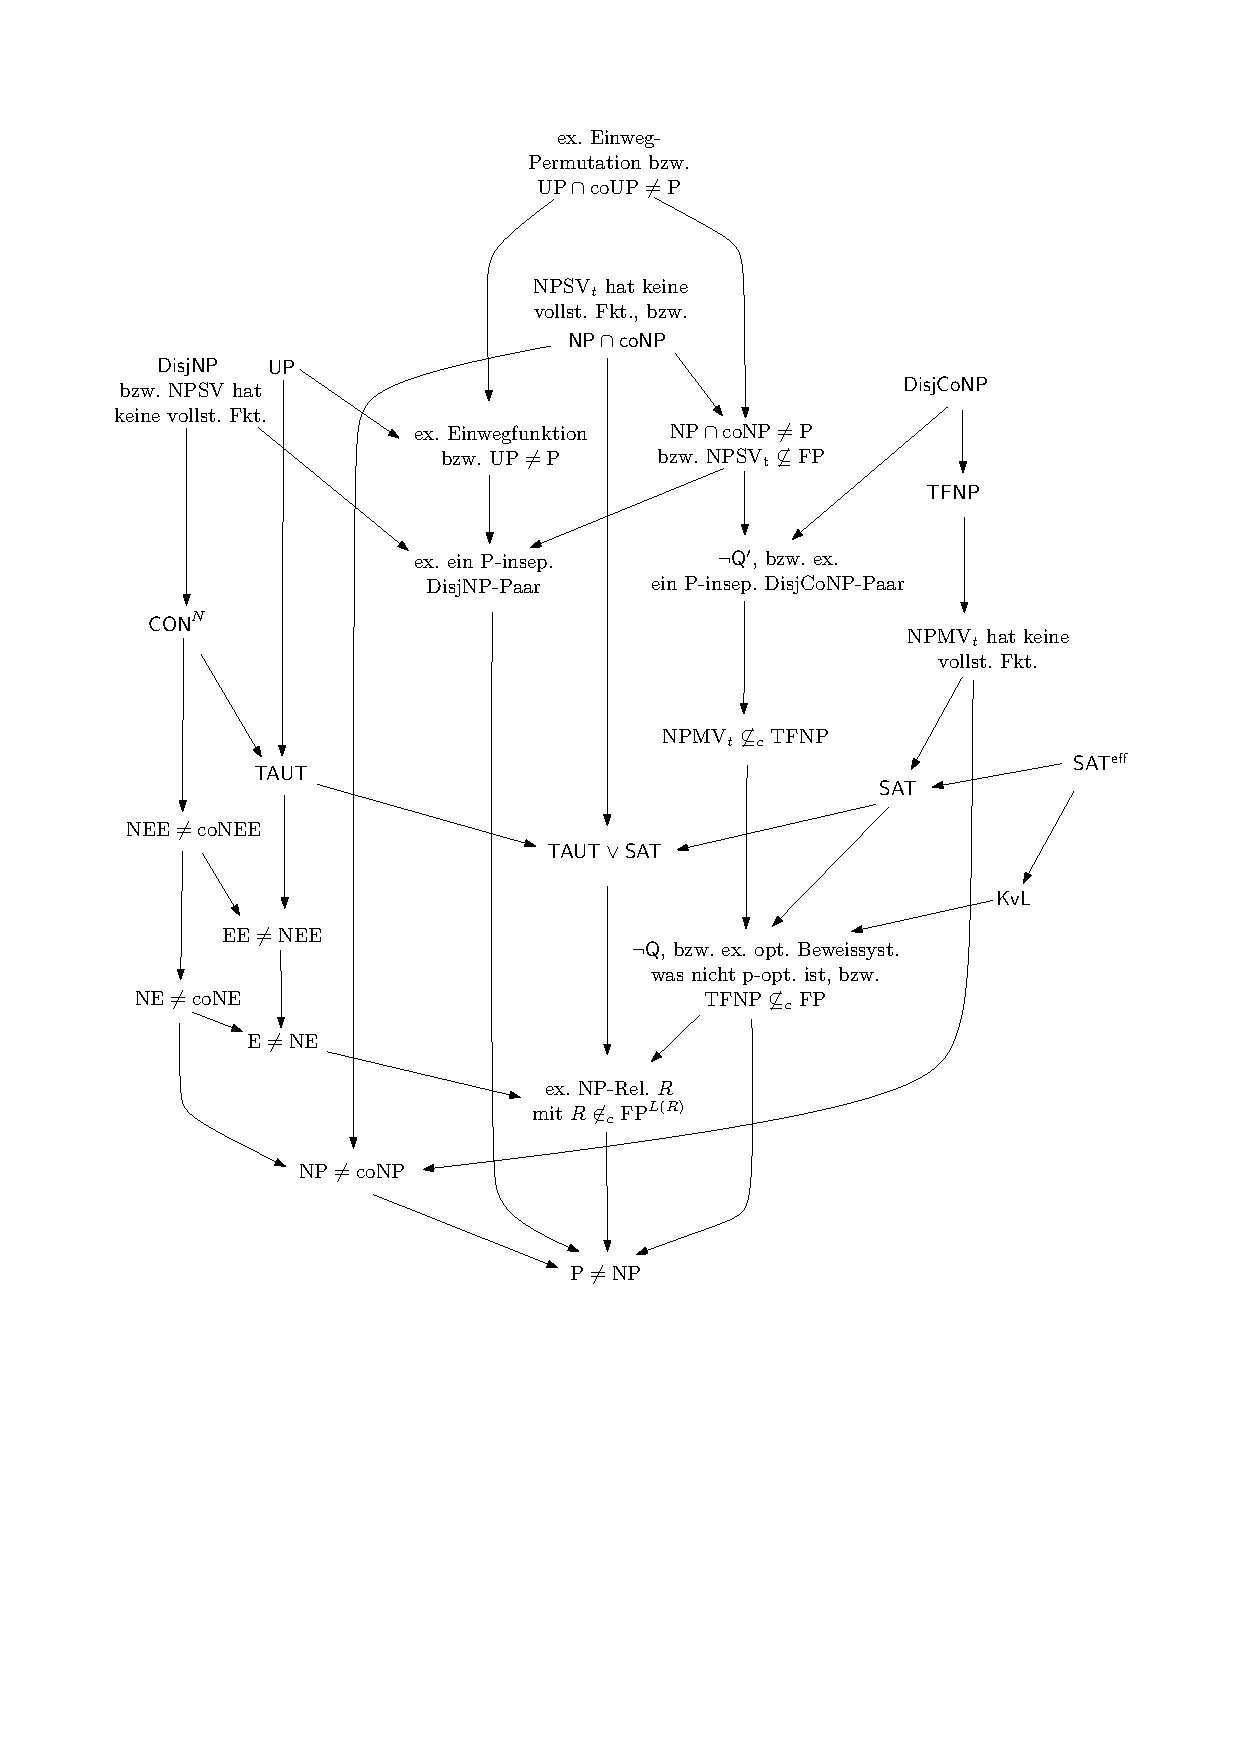
\includegraphics[page=1]{figures.pdf}
    \caption{Bekannte (relativierenden) Implikationen zwischen den betrachteten Hypothesen und weiteren Aussagen. Satz~\ref{thm:figure-implications} gibt Belegstellen für jede dieser Implikationen an.}\label{fig:figure-implications}
\end{figure}

\begin{theorem}\label{thm:figure-implications}
    Es gelten die in Abbildung \ref{fig:figure-implications} abgebildeten Implikationen und Äquivalenzen.
\end{theorem}
\begin{proof}
    Es gelten die notiertern Äquivalenzen:
    \begin{Prooflist}[nosep]
    \item $\neg\hQ \Leftrightarrow \mathit{sat}$ ist p-optimal, nach Satz~\ref{thm:q}.
    \item $\NP\neq\coNP \Leftrightarrow$ existiert keine NP-harte Funktion in $\TFNP$, nach Satz~\ref{thm:tfnp-vs-npconp}.
    \item $\neg\hQ' \Leftrightarrow\exists$ P-inseparierbares $\DisjCoNP$-Paar, nach \textcite{fortnow_separability_2002}.
    \item $\NP\cap\coNP\neq\P \Leftrightarrow \NPSV_t\not\subseteq\FP$, nach \textcite{selman_taxonomy_1994}.
    \item $\UP\neq\P \Leftrightarrow\exists$ Einwegfunktionen, nach \textcite[Thm.~10]{grollmann_complexity_1988}.
    \item $\UP\cap\coUP\neq\P \Leftrightarrow\exists$ Einwegpermutationen, nach \textcite{homan_one-way_2003}.
    \item $\hNPcoNP \Leftrightarrow \NPSV_t$ hat keine vollständige Funktion, nach \textcite[Prop.~3]{beyersdorff_nondeterministic_2009}.
    \item $\hDisjNP \Leftrightarrow \NPSV$ hat keine vollständige Funktion, nach \textcite[Thm.~9]{glaser_reductions_2005}.
    \end{Prooflist}

    Es gelten die eingezeichneten Implikationen:
    \begin{Prooflist}[nosep]
\item $\hDisjNP \Rightarrow \mathsf{CON}^N$ nach \textcite{kobler_optimal_2003}.
\item $\hUP \Rightarrow \hTAUT$ nach \textcite{kobler_optimal_2003}.
\item $\mathsf{CON}^N\Rightarrow \mathrm{NEE\neq coNEE}$ nach \textcite{kobler_optimal_2003}.
\item $\NP\cap\coNP\neq \P \Rightarrow \neq\hQ' \Rightarrow \NPMVt \not\subseteqc \TFNP \Rightarrow \neq\hQ$ nach \textcite{fenner_inverting_2003}.
%\item $\mathrm{E\neq NE}\Rightarrow \exists$ NP-Relation die nicht auf Entscheidung reduzierbar ist, nach \textcite{bellare_complexity_1994}.
\item $\mathrm{E\neq NE}\Rightarrow \exists$ NP-Relation die nicht auf Entscheidung reduzierbar ist, nach \textcite{impagliazzo_1991}.
\item $\UP\neq\P \Rightarrow \exists$ P-inseparierbares $\DisjNP$-Paar, nach \textcite[Thm.~5]{grollmann_complexity_1988}.
\item $\hNPcoNP\Rightarrow \hTAUT\lor\hSAT$ nach \textcite{beyersdorff_nondeterministic_2009}.
\item $\NPMVt$ hat keine vollständige Funktion $\Rightarrow \hSAT$ nach \textcite[Thm.~25]{beyersdorff_nondeterministic_2009}.
\item $\NPMVt$ hat keine vollständige Funktion $\Rightarrow \NP\neq\coNP$ nach Satz~\ref{thm:tfnp-vs-npconp}.
\item $\mathsf{SAT^{eff}} \Rightarrow \hSAT, \mathsf{SAT^{eff}}\Rightarrow \mathsf{KvL}$, nach Satz~\ref{thm:sateff-generalizes-sat}.
\item $\mathsf{KvL}\Rightarrow\neg\hQ$, nach Satz~\ref{thm:kvl-implies-q}.
\item $\neg\hQ\Rightarrow \exists$ NP-Relation die nicht auf Entscheidung reduzierbar ist, denn unter $\neg\hQ$ gilt mit Satz~\ref{thm:q} auch die Negation von \ref{thm:q}(1), also eine NPTM $N$ mit $L(N)=\Sigma^*$ wobei keine Funktion $g\in\FP$ existiert, welche für alle $x$ durch $g(x)$ einen akzeptierenden Rechenweg von $N(x)$ bestimmt.
    Definiere die NP-Relation $R_N$ mit $(x,\alpha)\in R_N$ genau dann wenn $N(x)$ mit Rechenweg $\alpha$ existiert. Nun gilt nach Vorigem auch $R\not\inc \FP=\FP^{\Sigma^*} = \FP^{L(R)}$.
\item $\hDisjCoNP \Rightarrow \hTFNP \Rightarrow \NPMVt$ hat keine vollständig Funktion, nach \textcite{pudlak_incompleteness_2017}.
\item $\NP\cap\coNP\neq \P \Rightarrow\exists$ P-inseparierbares $\DisjNP$-Paar, denn wenn alle $\DisjNP$-Paare P-separierbar, dann ist auch für jede Menge $L\in\NP\cap\coNP$ jeweils das $\DisjNP$-Paar $(L,\overline{L})$ P-separierbar und damit $L\in\P$.
\item $\hDisjNP \Rightarrow \exists$ P-inseparierbares $\DisjNP$-Paar; ist klar, denn wenn alle $\DisjNP$-Paare P-separierbar wären, dann wären auch alle Paare $\leqmpp$-vollständig.
\item $\hDisjCoNP \Rightarrow \exists$ P-inseparierbares $\DisjCoNP$-Paar; ist aus selben Gründen klar.
\item $\mathsf{CON}^N \Rightarrow \hTAUT$ klar, weil aus p-Optimalität auch Optimalität folgt.
\item $\mathsf \hSAT \Rightarrow \neg\hQ $ klar, denn wenn $\mathit{sat}$ p-optimal ist, dann existiert \emph{ein} p-optimales Beweissystem für $\mathtt{SAT}$.
\item $\hUP \Rightarrow \UP\neq\P$ klar.
\item $\hNPcoNP \Rightarrow \NP\cap\coNP\neq \P$ klar.
\item $\exists$ P-inseparierbares $\DisjNP$-Paar $\Rightarrow \P\neq \NP$ klar.
\item $\UP\cap\coUP\Rightarrow \UP\neq \P$, $\UP\cap\coUP\Rightarrow \NP\cap\coNP\neq\P$ klar.
\item $\mathrm{NEE\neq coNEE \Rightarrow NE \neq coNE \Rightarrow NP \neq coNP \Rightarrow P\neq NP}$ klar.
\item $\mathrm{NEE\neq coNEE \Rightarrow EE \neq NEE \Rightarrow E\neq NE}$ klar.\qedhere
\end{Prooflist}
\end{proof}

\chapter{Orakel}


\note{Abschließend erweitern wir noch unsere Notation, die uns insbesondere bei der Orakelkonstruktion helfen wird. Diese folgt Überlegungen von \textcite{dose_np-completeness_2019}. Anstelle von Orakeln als Menge zu verstehen, können wir äquivalent Orakel auch als unendlich lange Wörter $u\in\Sigma^\omega$ formulieren, die wir als das Orakel $\{ i\mid w[i]=1 \}\subseteq \mathbb N$ interpretieren. Mit der obigen Identifikation von Wörtern und natürlichen Zahlen beschreibt nun $u$ sowohl ein Orakel über $\mathbb N$ als auch über $\Sigma^*$; wir können also z.B. von der relativen Berechnung $M^w(x)$ sprechen. Analog fassen wir endlich lange Wörter $w\in\Sigma^*$ als \emph{partielles} Orakel $\{ i\mid w[i]=1 \}$, welches die Zugehörigkeit der Wörter $x<|w|$ festlegt, aber die Zugehörigkeit aller Wörter $y\geq|w|$ noch nicht endgültig festlegt.
Auf dieser Idee der endgültigen bzw. noch nicht endgültigen Zugehörigkeit aufbauend können wir auch von \emph{definiten} Berechnungen sprechen: Eine Rechnung $M^w(x)$ ist \emph{definit} wenn auf allen Rechenwegen von $M^w(x)$ nur Orakelfragen gestellt werden, welche eine Länge $<|w|$ haben. }
